\documentclass[paper=a4,fontsize=12pt,ngerman,bibliography=totoc,parskip=half]{scrartcl}

% should be loaded early
\usepackage[T1]{fontenc}
\usepackage[utf8]{inputenc}

\usepackage{amsfonts}
\usepackage{amsmath}
\usepackage{amssymb}
\usepackage[ngerman]{babel}
\usepackage{booktabs}
\usepackage{csquotes}
\usepackage{hyperref}
\usepackage{lmodern}
\usepackage{tabularx}
\usepackage{tikz}
\usepackage{todonotes}
\usepackage{placeins}

\usepackage[bibstyle=numeric,citestyle=numeric,backend=biber]{biblatex}
\bibliography{studienarbeit}

\usepackage{color}
\usepackage{xcolor}
\definecolor{dkgreen}{rgb}{0,0.6,0}
\definecolor{gray}{rgb}{0.5,0.5,0.5}
\definecolor{lightgrey}{rgb}{0.95,0.95,0.95}
\definecolor{mauve}{rgb}{0.58,0,0.82}

% settings for listing
\usepackage{listings}
\lstset{ %
language=Java,                % choose the language of the code
basicstyle=\footnotesize,    % the size of the fonts that are used for the code
%basicstyle=\small,
numbers=left,                % where to put the line-numbers
numberstyle=\tiny\color{gray},      % the size of the fonts that are used for the line-numbers
stepnumber=1,                   % the step between two line-numbers. If it is 1 each line will be numbered
numbersep=5pt,                  % how far the line-numbers are from the code
backgroundcolor=\color{lightgrey},  % choose the background color. 
showspaces=false,               % show spaces adding particular underscores
showstringspaces=false,         % underline spaces within strings
showtabs=false,                 % show tabs within strings adding particular underscores
frame=single,           % adds a frame around the code
tabsize=2,          % sets default tabsize to 2 spaces
captionpos=b,           % sets the caption-position to bottom
breaklines=true,        % sets automatic line breaking
breakatwhitespace=false,    % sets if automatic breaks should only happen at whitespace
escapeinside={\%*}{*)},          % if you want to add a comment within your code
keywordstyle=\color{blue},          % keyword style
commentstyle=\color{dkgreen},       % comment style
stringstyle=\color{mauve}         % string literal style
}
% for utf8 encoding
\lstset{literate=%
    {Ö}{{\"O}}1
    {Ä}{{\"A}}1
    {Ü}{{\"U}}1
    {ß}{{\ss}}1
    {ü}{{\"u}}1
    {ä}{{\"a}}1
    {ö}{{\"o}}1
    {~}{{\textasciitilde}}1
}

 % for an empty page after each section
\usepackage{titlesec}
\newcommand{\sectionbreak}{\clearpage}

% für theoreme, definitionen, etc
\usepackage{ntheorem}
\theoremstyle{break} % new linebreak before content of theorem starts 
\newtheorem*{definition}{Definition}
\newtheorem{proof}{Beweis}
\newtheorem{theorem}{Satz}

% um Umbruchprobleme zu vermeiden - erlaubt ggf längere Zeilen
\setlength{\emergencystretch}{1em} 
\hyphenation{all-er-dings}
\hyphenation{aus-zu-wäh-len}
\hyphenation{gleich-wohl}

% eigene Befehle
\newcommand{\code}[1]{\textsf{#1}}

% subsubsections und tiefer nicht ins inhaltsverzeichnis
\setcounter{tocdepth}{3}

% Dokumenteneigenschaften
\title{Studienarbeit}
\subtitle{Vereinfachung und Automatisierung\\ der Datenverwaltung für Semedico}
\author{Philipp Lucas}
\date{Friedrich-Schiller-Universität Jena\\ Fakultät für Mathematik und Informatik \\
\today}%27.\,09.~2012}

\begin{document}

% für tikz
\usetikzlibrary{shapes,arrows}
\usetikzlibrary{positioning}
\tikzstyle{decision} 	= [diamond, draw, fill=blue!20, text badly centered, node distance=3cm, inner sep=0pt]
%\tikzstyle{decision} 	= [diamond, draw, fill=blue!20, text width=4.5em, text badly centered, inner sep=0pt]
\tikzstyle{block} 	= [rectangle, draw, fill=blue!20, text width=10em, text centered, rounded corners, minimum height=4em]
\tikzstyle{line} 	= [draw, -latex']
\tikzstyle{cloud} 	= [draw, ellipse,fill=red!20, node distance=3cm,minimum height=2em]
\tikzstyle{decision answer}=  [near start, color=black]

\maketitle


%\newpage
\tableofcontents
%\newpage

\section{Einleitung}

An dem Language and Information Engineering Lab (JULIE Lab) der Friedrich-Schiller-Universität Jena (FSU Jena) wird seit 2008 an dem Semedico-Projekt gearbeitet. Ziel ist es, eine semantische Suchmaschine zu entwickeln, welche es dem Nutzer ermöglicht schneller und gezielter als mit klassischen Suchmaschinen relevante Veröffentlichungen der Biomedizin zu finden.

%Semedico grenzt sich von anderen Suchmaschinen   

%Eines der wesentlichen Probleme beim wissenschaftlichen Arbeiten ist die Informationssuche. Verschiedenen Studien zufolge verbringt ein Wissenschaftler 50\,\% bis 60\,\% seiner Arbeitszeit mit der Suche nach passenden Informationen TODO:cite. Dieses Problem wird umso größer als die Menge an Daten und Wissen weiterhin exponentiell wächst TODO:cite. Der logische Schluss ist es Methoden zu entwickeln, die es erlauben schnell und gezielt relevante Informationen zu finden. \par

%Eben zu diesem Zweck wird am Language and Information Engineering Lab (JULIE Lab) der Friedrich-Schiller-Universität Jena (FSU Jena) die semantische Suchmaschine Semedico entwickelt.

Semedico baut dabei auf eine Vielzahl von Daten auf, insbesondere aber auf die Medical Subject Headings (MeSH), ein Thesaurus zur Sacherschließung von Texten aus der Medizin und den Biowissenschaften. \par

In der hier vorgelegten Studienarbeit wurde eine Software erarbeitet, die die Verwaltung der verschiedenen Datenquellen des Semedico-Systems vereinheitlicht und vereinfacht. Dies schließt Algorithmen ein, die das Upgrade des MeSH von einer Version zur nächsten vollständig automatisieren. \par 

%\subsection{Semedico}
%\label{sec:semedico}

\minisec{Medical Subject Headings}
Der MeSH ist ein jährlich vom National Library of Medicine (NLM) herausgegebener polyhierarchischer Thesaurus. Er dient zum Katalogisieren von Medien sowie insbesondere zum Indizieren von biomedizinischen Veröffentlichungen. Nach Angaben der offiziellen Webseite werden Artikel von 5\,400 der weltweit führenden biochemischen Journals mit Hilfe des MeSH indiziert \cite{MeSHWeb2012}. \par

Der MeSH enthält Entry Terms, welche jeweils einem Descriptors zugeordnet sind. Zusammen bilden sie eine nach Spezifizität geordnete Polyhierarchie \cite{MeSHWeb2012}. Allgemeine Begriffe wie beispielsweise "`Organisms"' sind folglich weit oben in der Hierarchie zu finden, während spezifischere Begriffe wie zum Beispiel "`Hepatitis Viruses"' diesen untergeordnet sind. \par

Für das Semedico-Projekt dient der MeSH als eine der wesentlichen Datenquellen, da die hierarchische Struktur des MeSH in abgewandelter Form auch als Wissensbasis für Semedico dient. Diese Abwandlung ist insbesondere notwendig, um für Semedico nicht relevante Terme zu entfernen. Zu Veranschaulichung: Der MeSH enthält etwa 200\,000 Entry Terms, welche jeweils einem der über 26\,000 Descriptors zugeordnet sind. Im für Semedio angepassten MeSH finden sich lediglich noch knapp 5\,000 Entry Terms und etwa eben so viele Descriptors.

% \subsubsection{Struktur}
% Es liegen zwei verschiedene Formate vor in denen der MeSH bezogen werden kann: als ASCII-Records sowie als XML-formatierte Records. Tatsächlich enthält die XML-Version einige Daten die in der ASCII-Version nicht vorliegen. \ldots


\minisec{Anmerkung zur Sprache}
Aus Gründen der Lesbarkeit und um Verwirrungen zu vermeiden, werden in dieser Arbeit durchgehend die englischen Originalbezeichnungen von MeSH-spezifischen Begriffen verwendet. \par

Quelltext und Kommentare der entwickelten Software sind vollständig in Englisch. Daher werden Bezeichnungen von Funktionen die eine direkte Entsprechung im Quellcode finden ebenfalls in Englisch bezeichnet. \par 

Abgesehen davon ist die Arbeit vollständig in Deutsch verfasst.

\section{Problemstellung}
\label{sec:problemstellung}
\subsection*{Verwaltung der Semedico-Wissensbasis}
Semedico kann als semantische Suchmaschine nur dann effektiv arbeiten, wenn ihr entsprechende Daten als Wissensbasis zur Verfügung stehen. Diese Daten umfassen im Moment unter anderem Daten aus dem MeSH und aus UniProt (eine umfassende Proteindatenbank \cite{Consortium2011}).\par
Eine Zielstellung dieser Studienarbeit ist es daher, eine einheitliche und vereinfachte Verwaltung der Datenquellen für Semedico zu entwickeln. Dies umfasst das Importieren von Daten unterschiedlichen Formats, die Repräsentation dieser Daten in internen Datenstrukturen, und auch den Export zu Semedico. \par

\autoref{sec:software} \textit{\nameref{sec:software}} beschreibt die dazu entwickelte Software.

\subsection*{Erstellen des Semedico-MeSH}
\label{sec:MeSH_erstellen}
Semedico hilft passende biomedizinische Publikationen zu finden, indem es dem Nutzer ermöglicht, Suchbegriffe mit klar definierter Bedeutung auf hierarchische Weise auszuwählen. %Dabei baut es eben auf Datenquellen wie den MeSH auf, um dem Nutzer zu ermöglichen exakte Anfragen zu stellen. 
Das ist möglich, weil diese Paper zuvor mit Hilfe des MeSH verschlagwortet wurden. Allerdings enthält der MeSH weitaus mehr als nur biomedizinische Fachtermini. Es sind ebenso unzählige andere Begriffe enthalten, welche für diese Anwendung überflüssig sind und sich sogar nachteilig auf die Performance bzw. Benutzbarkeit auswirken würden. 
Es ist also erforderlich aus der Gesamtheit des MeSH eine Teilmenge auszuwählen. Diese Teilmenge wird fortan Semedico-MeSH genannt. \par

Im JULIE Lab existiert bereits ein Algorithmus der diese Auswahl vornimmt. Allerdings ist er aufgrund fehlender Dokumentation, aufwendiger, d.\,h. teil-manueller, bzw. unklarer Handhabung und schlechter Flexibilität auf mittlere und längere Sicht unbrauchbar. Das Ergebnis dieses Algorithmus', angewandt auf den MeSH 2008, liegt vor und soll soweit möglich reproduziert werden. \par

Zum einen müssen also die aktuell vorhandenen Algorithmen und Daten analysiert werden, um herauszufinden welche Operationen den MeSH 2008 in den Semedico-MeSH 2008 überführen. \ref{sec:mesh} \textit{\nameref{sec:mesh}} beschreibt dazu die Grundlagen, und \ref{sec:vergleichBaume} \textit{\nameref{sec:vergleichBaume}} beschäftigt sich hiermit. \par

Zum anderen müssen Methoden entwickelt werden, die diese Operationen, wie zum Beispiel Hinzufügen, Löschen oder Verschieben, auf importierte Daten anwenden, sowie solche, die diese Operationen extern abspeichern und wieder einlesen können. Siehe dazu \autoref{sec:software}.\par

\subsection*{Aktualisierung des Semedico-MeSH}
\label{sec:aktualisierung_semedico} 
Die National Library of Medicine veröffentlicht jährlich eine neue, aktualisierte Version des MeSH. Diese Aktualisierung umfasst unter anderem das Hinzufügen neuer Begriffe, das Löschen obsoleter Begriffe oder das Aufteilen eines Begriffs in mehrere. Wie im vorangegangenen Abschnitt erklärt, wird der Semedico-MeSH aus dem MeSH erstellt, indem eine Folge von Operationen angewandt wird. Diese Operationen können durch die Aktualisierung des MeSH unanwendbar geworden sein. Beispielsweise kann ein Element, das verschoben werden soll, fehlen. \par

Um eine aufwendige, manuelle Korrektur der Operationen zu vermeiden, sollen in dieser Studienarbeit Methoden entwickelt werden, welche voll-automatisiert eine syntaktische Korrektur vornehmen, während sie die Semantik so belassen, wie sie im aktualisierten MeSH vorgegeben ist. Das Vorgehen zur Lösung dieses Problems wird in \autoref{sec:merging} \textit{\nameref{sec:merging}} beschrieben.

% \subsection{Auflistung}
% \begin{itemize}
%   \item Analyse der vorhandenen Methoden zur Erzeugung des MeSH
%   \item Identifikation der relevanten Semedico-MeSH-Daten
%   \item Implementieren von Methoden zum Import und Export von Daten unterschiedlicher Quellen
%   \item Implementierung einer adäquaten Repräsentation des MeSH als Baum aus Tree Vertices sowie Menge von Descriptors
%   \item Aufbau einer Grundbibliothek zum Verwalten und Verändern eines Baumes
%   \item Implementierung von Methoden zum Vergleich zweier Bäume. Ziel: Finden der angewandten Operationen
%   % 		* unter Kriterium: möglichst wenig Operationen / "möglichst semantisch logisch"
% % 		* Spezialfall: Ud-MeSH-XML
% % 		* Allgemeiner Fall
% \item Korrektur einer Operationsmenge
% \end{itemize}

\section{Grundlagen}

\subsection{MeSH}
\label{sec:mesh}
%Sinn und Bedeutung des MeSH wurden bereits in \autoref{sec:semedico} erläutert. 
In diesem Abschnitt wird die interne Struktur des MeSH beschrieben.

\subsubsection{MeSH Record Types}
%http://www.nlm.nih.gov/mesh/intro_record_types.html

\minisec{Descriptors}
Wie bereits in der Einleitung erwähnt, bildet der MeSH eine hierarchische Struktur, deren zentrales Element sogenannte Descriptors sind. Ein Descriptor ist die Repräsentation eines Begriffs bzw. eines Begriffsraumes für den im MeSH ein Index-Eintrag existiert. Descriptors haben eine teils mehr, teils weniger scharf abgegrenzte Bedeutung, je nach dem wie dies aus Sicht der Autoren des MeSH zur Zeit den Anforderungen des Wissenschaftbetriebs entspricht. Mehr Informationen zu den Organisationsprinzipien finden sich in \cite{MeSHOrgPrinciples2012}.\par

Neben den Descriptors gibt es zwei weitere sogenannte MeSH Record Types, die jedoch für diese Arbeit nicht von Interesse sind: Qualifiers und Supplementary Concept Records (SCR).\par

\minisec{Qualifiers}
Es existieren insgesamt 83 thematische Qualifiers. Sie erlauben es, im Zusammenspiel mit Descriptors, bestimmte Aspekte eines Themas sinnvoll zu gruppieren. Beispielsweise weist der Qualifier "`Liver/drug effects"' darauf hin, dass sich ein Artikel nicht allgemein mit der Leber, sondern mit den Auswirkungen von Medikamenten beschäftigt.

\minisec{Supplementary Concept Records}
Die Supplementary Concept Records (SCR) werden vor allem genutzt, um Chemikalien und Medikamente zu indizieren. Während sie grundsätzlich sehr ähnliche Attribute besitzen, besteht der wesentliche Unterschied zu Descriptors darin, dass SCRs keine Tree Numbers besitzen und sie folglich nicht selbst eine Hierarchie bilden. Stattdessen werden sie jeweils einem oder mehreren Descriptors zugeordnet und ergänzen bzw. spezifizieren so dessen Bedeutung. \par
%Es gibt mehr als 200\,000 SCR Einträge mit mehr als 500\,000 SCR terms.

\subsubsection{MeSH Komponenten und XML}
\label{sec:xml_struktur}
Der MeSH ist in zwei Formaten verfügbar: als XML-File sowie als ASCII-File. In dieser Arbeit wird die XML-Version verwendet, da zum einen die XML-Format reicher als die ASCII-Format ist \cite{Nelson2004}, und da zum anderen durch die Verwendung der seitens der NLM bereitgestellten dtd-Datei ein validiertes Parsen möglich ist. 

Nachfolgend werden die wichtigsten Begriffe im MeSH, nämlich Descriptor, Tree Number, Concept und Term für sich selbst und als XML-Element erklärt. \autoref{fig:MeSH_structure} zeigt den strukturellen Aufbau (der hier wichtigen Elemente) des MeSH. \par

Für eine detaillierte und vollständige Beschreibung aller XML-Elemente wird auf \cite{MeSHXML2012} verwiesen.\par

\begin{figure}[h]
\begin{center}
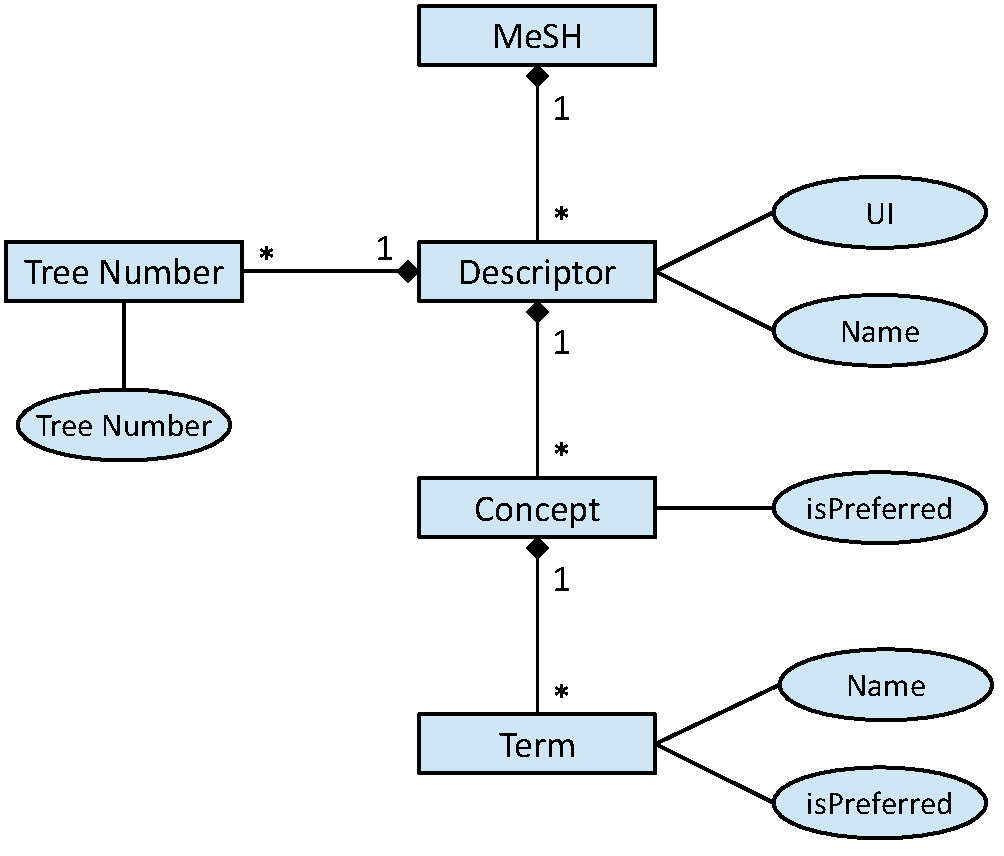
\includegraphics[width=0.8\textwidth]{figs/MeSH_structure_neu.pdf}
\end{center}
\caption{Datenstruktur des MeSH}
\label{fig:MeSH_structure}
\end{figure}

\minisec{MeSH}
Wenn man von SCRs absieht, besteht der MeSH aus einer Menge von Descriptors. Das entsprechende XML-Root-Element ist \code{<DescriptorRecordSet>}, welches alle Descriptors als direkte Kinder enthält.

\minisec{Descriptor}
Die Bedeutung der Descriptors wurde bereits weiter oben diskutiert.\par

Ein Descriptor als XML-Element ist ein \code{<DescriptorRecord>} und besteht, unter anderem, aus einer Menge von Tree Numbers (XML-Element: \code{<TreeNumberList>}) sowie aus einer Menge von Concepts (XML-Element: \code{<ConceptList>}). Tree Numbers betten Descriptors in eine oder mehrere Positionen in der Begriffshierarchie ein. Concepts erlauben eine feinere Einteilung der Bedeutung eines Descriptors.\par

Ein Descriptor kann eindeutig durch seine UI (XML-Element: \code{<DescriptorUI>}) und seinen Namen (XML-Element \code{<DescriptorName>}) identifiziert werden. Der Name ist dabei der  \code{<PreferredName>} des \code{<PrefferedConcepts>} des Descriptors.\par

Es sind keine expliziten Relationen, wie zum Beispiel Inklusion auf Descriptors, definiert. Siehe dazu auch den Abschnitt unten zu Tree Numbers. \par

Ein Descriptor wird auch als Descriptor Record oder Main Heading bezeichnet.

\minisec{Concept}
Ein Concept besteht aus einer Menge von Terms und kann über seine ID (XML-Element \code{<ConceptUI>}) eindeutig identifiziert werden. \par

Ein Concept beschreibt eine begriffliche Untereinheit eines Descriptors. Alle Terme innerhalb eines Concepts sind synonym zueinander. \par

\minisec{Tree Number}
Eine Tree Number ist eine alpha-numerische Zeichenkette und verweist an einer bestimmte Position des MeSH auf den Descriptor, der diese Tree Number enthält. Das dazugehörige XML-Element ist  \code{<TreeNumber>}. \par
% Beispiel:
% \begin{verbatim}
% <TreeNumber>C02.839.040</TreeNumber>
% \end{verbatim}
Es ist an dieser Stelle zu bemerken, dass die hierarchische Struktur des MeSH nicht explizit als XML-Element vorliegt. Vielmehr ergibt sich die Struktur allein implizit durch die Namensgebung der Tree Numbers, also eben aus der Eigenschaft, dass eine Tree Number $x.y.z$ dafür steht, dass die Tree Number $x.y$ der Vater der Tree Number $x.y.z$ ist. \par

Diese Verflechtung von ID einer Tree Number und Strukturinformation ist aus unserer Sicht nicht wünschenswert: Unter Aufrechterhaltung dieser Eigenschaft führt ein lokales Verändern der hierarchischen Struktur zu nicht-lokalen Änderungen der Tree Number. Beispielsweise führt ein Verschieben einer Tree Number dazu, dass auch alle untergeordneten Tree Numbers umbenannt werden. Das macht ein Arbeiten mit der Hierarchie unnötig kompliziert. In \autoref{sec:repräsentation_des_mesh_als_baum} wird eine Möglichkeit diskutiert, wie diese Verflechtung beseitigt werden kann. \par

\minisec{Term}
Ein Term wird auch als Entry Term bezeichnet. Und \cite{MeSHEntryTerms2012} beschreibt Entry Terms folgendermaßen:
\begin{quotation}
"`Entry terms, sometimes called "`See cross-references"' in printed listings, are synonyms, alternate forms, and other closely related terms in a given MeSH record that are generally used interchangeably with the preferred term for the purposes of indexing and retrieval, thus increasing the access points to MeSH-indexed data."'
\end{quotation}

Das dazugehörige XML-Element ist  \code{<Term>}. 

%\subsubsection {MeSH Struktur}
%MeSH-Descriptors sind, indirekt über ihre Tree Numbers, in 16 Bäumen angeordnet. Die Wurzeln der Bäume werden auch Kategorien genannt und bezeichnen grundlegende Konzepte, wie beispielsweise "`A (Anatomy)"' oder "`B (Organisms)"'. Diese Wurzeln sind allerdings nicht als Descriptor im MeSH repräsentiert. Jede Kategorie besitzt Unterkategorien, etwa "`A01 (Body Regions)"', in welchen die Tree Numbers der Descriptors angeordnet sind. Je tiefer eine Tree Number dabei in einem Baum liegt, desto spezieller ist die Bedeutung des dazugehörigen Descriptors im Kontext des Astes, in dem die Tree Number liegt. Siehe dazu auch \autoref{fig:MeSH_structure}.

\subsubsection{Jährliche Änderungen}
\label{sec:anual_changes}
Jedes Jahr erscheint eine neue, an die aktuellen Entwicklungen der Wissenschaft angepasste Version des MeSH. Auch für Semedico soll die jeweils aktuelle Version des MeSH als Datengrundlage verwendet werden. Dazu wird, wie zuvor in \autoref{sec:MeSH_erstellen} erklärt, eine Folge von Operationen auf den MeSH angewandt, um daraus den Semedico-MeSH zu erzeugen. Problematisch ist hierbei, dass mit jeder Änderung am MeSH die Operationen zur Erzeugung des Semedico-MeSH potentiell unmöglich werden. Beispielsweise kann eine Tree Vertex nicht mehr verschoben werden, falls sie in der neuen Version des MeSH nicht mehr existiert.\par

\minisec{Lösungsmöglichkeiten}

\begin{figure}
\begin{center}
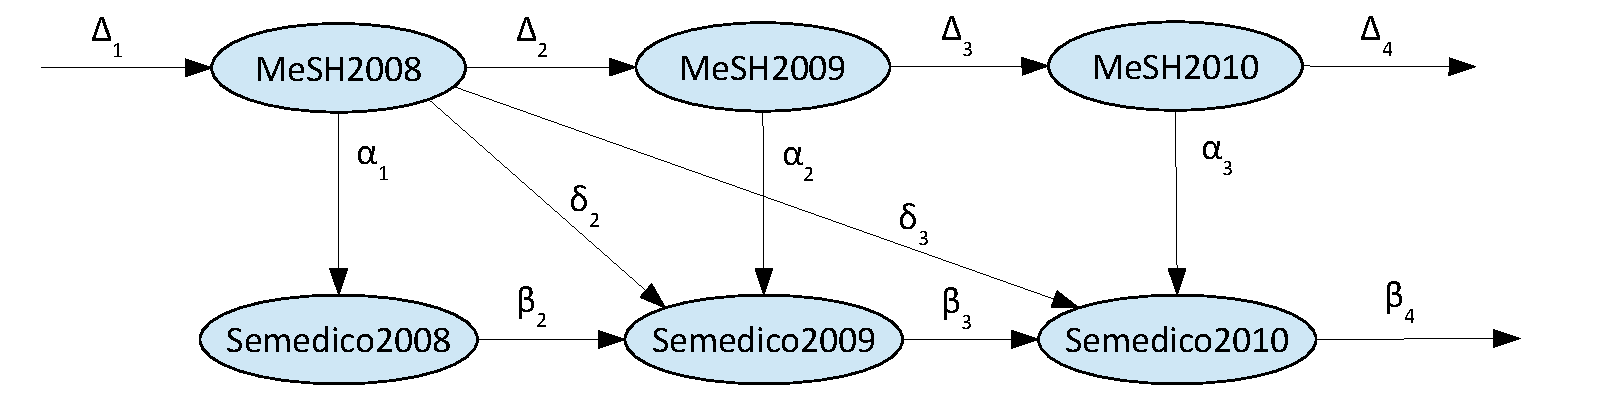
\includegraphics[width=0.9\textwidth]{figs/anualChangesConcepts.pdf}
\end{center}
\caption{Möglichkeiten zur Erzeugung des jährlichen Semedico-MeSH}
\label{fig:anualChangesConcept}
\end{figure}

\autoref{fig:anualChangesConcept} zeigt schematisch die Lösungsvarianten, die nachfolgend konzeptionell erläutert werden. \par

Gegeben sind \code{MeSH2008} sowie \code{Semedico2008}, also der MeSH des Jahres 2008 und der darauf basierende Semedico-MeSH. Daraus kann $\alpha_1$ bestimmt werden und ist damit ebenfalls gegeben. $\Delta_i$, $\alpha_i$, $\beta_i$, $\delta_i$ seien Operationsfolgen, die einzelne Versionen des MeSH, wie in \autoref{fig:anualChangesConcept} dargestellt, ineinander überführen. Ziel ist es, den Semedico-MeSH für die Folgejahre zu erstellen. Um das zu erreichen, gibt es wenigstens drei Möglichkeiten:
\begin{itemize}
  \item[$(\alpha)$] Den MeSH des aktuellen Jahres in den Semedico-MeSH überführen. Dazu wird $\alpha_i$ als Aktualisierung von $\alpha_{i-1}$ unter Zuhilfenahme von $\Delta_i$ erstellt.
  \item[$(\beta)$] Den Semedico-MeSH des vorangegangen Jahres aktualisieren. Hierzu wird $\beta_i$ als modifizierte Teilmenge von $\Delta_i$ erstellt - als Menge all der Operationen aus $\Delta_i$ die auf \code{Semedico20xx} angewandt werden können. 
  \item[$(\delta)$] Direkt aus dem MeSH2008 den aktuellen Semedico-MeSH erzeugen. Dafür wird $\delta_i$ als Vereinigung von $\delta_{i-1}$ und $\Delta_i$ erzeugt.
\end{itemize}

Für diese Studienarbeit wurde die erste Variante $(\alpha)$ umgesetzt. Zum einen werden also die jährlichen Änderungen $(\Delta)$ des MeSHs benötigt. In \autoref{sec:vergleichBaume} \textit{\nameref{sec:vergleichBaume}} wird beschrieben wie diese ermittelt werden. Zum anderen muss $\alpha$ aktualisiert werden. Das Vorgehen dazu ist in \autoref{sec:merging} \textit{\nameref{sec:merging}} erklärt. Als Basis werden hier in den restlichen Unterabschnitten dieses Abschnitts grundlegende Begriffe der Graphentheorie, eine Formalisierung des MeSH, sowie verschiedene Operationen und Relationen auf dem formalisierten MeSH eingeführt.

\minisec{Änderungen verfolgen} 
Online sind für die jeweils aktuelle Version Änderungslisten verfügbar. Allerdings sind diese weder umfassend noch vollständig\footnote{See "`4. MeSH Vocabulary Changes for 2013"' of \url{http://www.nlm.nih.gov/mesh/introduction.html}}. Das heißt sie enthalten nicht alle Informationen zu den Änderungen. Beispielsweise gibt es keine Informationen dazu \textit{welche} Attribute eines Descriptors geändert wurde, sondern nur, \textit{dass} er geändert wurde. Und sie enthalten auch nicht alle Änderungen. Beispielsweise gibt es überhaupt keine Informationen zu Aufteilungen von Descriptors. \par

Daher ist es notwendig eigene Methoden zu entwickeln, um diese Änderungen zu bestimmen. Siehe dazu \autoref{sec:vergleichBaume} \textit{\nameref{sec:vergleichBaume}}. 

\subsection{Graphentheorie}
Dieser Abschnitt definiert die klassischen Begriffe der Graphentheorie. Sie sind in wesentlichen Teilen~\cite{Diestel2010} entnommen.

\begin{definition}[Graph, Knoten, Kante]
%Ein Graph $G$ ist ein 2-Tupel $(V,E)$ mit $E \subseteq V \times V$. Die Elemente der Menge $V$ werden Knoten genannt. Die Elemente der Menge $E$ werden Kanten genannt. Sie sind geordnete Paare aus Elementen $V$s. 
Ein Graph $G$ ist ein 2-Tupel $(V,E)$ mit $E \subseteq V^2$. Die Elemente der Menge $V$ werden Knoten genannt. Die Elemente der Menge $E$ werden Kanten genannt. Ist $\{x,y\} \in E$, so bezeichnen wir diese Kante auch mit $xy$.
\end{definition}

\begin{definition}[Knotenmenge, Kantenmenge]
Sei $G=(W,F)$ ein Graph. Wir bezeichnen dann $E(G) = F$ als Kantenmenge und $V(G) = W$ als Knotenmenge $G$s.
% \begin{itemize}
%   \item[]$E(G) = W$ als Knotenmenge
%   \item[]$V(G) = F$ als Kantenmenge
% \end{itemize}
\end{definition}

\begin{definition}[Teilgraph]
Ein Graph $S$ heißt Teilgraph eines Graphen $G$ genau dann, wenn gilt
\[ 
 E(S) \subseteq E(G) \wedge V(S) \subseteq V(G)
\]
\end{definition}

\begin{definition}[Pfad, Zyklus, Kreis]
Ein Pfad $P$ in einem Graphen $G$ ist eine Folge von Knoten $(x_0,\ldots,x_k)$, so dass:
\begin{align*}
	\forall (i=0,\ldots,k-1) : x_ix_{i+1} \in E(G)  
\end{align*}

Die Länge des Pfades $P$ ist gleich $k-1$ und wird mit $l(P)$ bezeichnet.\par

Sei $s=x_0$ und $t=x_k$. Dann heißt $P$ auch $s-t$-Pfad.\par

Existieren $m,n \in \{0,\ldots,k\}$ so dass $x_m = x_n$, dann heißt $P$ Zyklus. \par

%Gelten $k>0$ und $x_0 = x_k$ und sind sonst alle $x_i$ verschieden, so heißt $P$ Kreis. \par
Gilt $x_0 = x_k$ und sind sonst alle $x_i$ verschieden, so heißt $P$ Kreis. \par
\end{definition}

\begin{definition}[Zusammenhängend]
Ein nicht leerer Graph heißt zusammenhängend, wenn er für je zwei seiner Knoten $x$ und $y$ einen $x-y$-Pfad enthält. 
\end{definition}

\begin{definition}[Baum, Wurzel]
Ein Graph $G$ heißt Baum, falls er zusammenhängend ist und es kein $S \subseteq V(G)$ mit $l(S) > 1$  gibt, so dass $S$ ein Kreis in $G$ ist.\par

In einem Baum $G$ gibt es einen beliebigen aber ausgezeichneten Knoten aus $V(G)$, der Wurzel genannt wird. Wir schreiben dafür auch $root(G)$.
\end{definition}

\begin{definition} [Tiefe eines Knotens]
Sei $G$ ein Baum und $v \in V(G)$. Sei weiter $P$ ein $root(G)-v$-Pfad. Dann setzen wir die Tiefe $v$s als $d(v) = l(P)$.  
\end{definition}

\begin{definition}[Verwandtschaft]
Zwei Knoten $x,y$ eines Baumes $G$ heißen benachbart oder adjazent, falls $xy \in E(G)$ gilt. \par

In einem Baum $G$ heißt ein Knoten $x$ Vater eines Knoten $y$ und der Knoten $y$ heißt Kind des Knotens $x$, falls gilt: 
\[ xy \in E(G) \wedge d(x) < d(y) \]

Die Menge aller Kinder eines Knoten $x$ wird auch als $children(x)$ und der Vater eines Knotens $x$ auch als $dad(x)$ bezeichnet. \par

In einem Baum $G$ heißt ein Knoten $x$ Vorfahre eines Knoten $y$ und der Knoten $y$ heißt Nachkomme des Knotens $x$ falls ein $x-y$-Pfad in $G$ existiert und $d(x) < d(y)$ gilt.
\end{definition}

\begin{definition}[Label und Typ]
 Ein Label besteht aus einem textuellem Schlüssel und einem beliebigen Wert, und wird einem Knoten oder einer Kante zugeordnet. \par

 Die Menge der Schlüssel der Label eines Knoten $v$ bzw. einer Kante $k$ wird als $label(v)$ bzw. $label(k)$ bezeichnet. \par 

 Den Wert eines Labels $l$ eines Knotens $v$ bzw. einer Kante $k$ identifizieren wir mit $v.l$ bzw. $k.l$. Ist der Wert von $l$ leer, so sagen wir auch $v$ bzw. $k$ sind vom Typ $l$. \par

 Ein Label erlaubt es damit Knoten und Kanten beliebige Zusatzinformationen zuzuordnen.
\end{definition}

% \minisec{Definitionen von \ldots }
% \begin{itemize}
%   \item Graph: gerichtet, ungerichtet
%   \item Vater, Mutter, Kind, Vorfahre, Nachkomme
%   \item Pfad
%   \item Baum
%   \item Wurzelknoten
%   \item Tiefe eines Knotens
% \end{itemize}


\subsection{Der MeSH als Graph}
\label{sec:repräsentation_des_mesh_als_baum}
%Ein MeSH wird in nachfolgend beschriebender Weise als Graph formalisiert. \par
Gegeben sei ein MeSH $M$. Dieser wird, wie nachfolgend beschrieben, als \textit{MeSH-Graph} $G_M$ formalisiert: 

\begin{itemize}
 \item Jeder Descriptor $d$ aus $M$ wird durch einen Knoten $v_d$ vom Typ \code{Descriptor} in $G_M$ repräsentiert. $v_d$ erhält zwei Label \code{name} und \code{ui} deren Werte der Name bzw. die UI von $d$ sind.
 \item Jede Tree Number $t$ aus $M$ wird durch einen Knoten $v_t$ vom Typ \code{TreeVertex} in $G_M$ repräsentiert. $v_t$ erhält ein Label \code{name} dessen Wert die tatsächliche Tree Number $t$ s ist. Weiterhin erhält $G_M$ eine Kante vom Typ \code{Descriptor} von $v_t$ nach $v_d$, wobei $v_d$ der Knoten ist durch den der Descriptor von $t$ repräsentiert wird.
 \item Für jedes Paar Tree Numbers $s$ und $t$ aus $M$, für die $s$ eine direkte Unterkategorie von $t$ ist, enthält $G_M$ eine Kante des Typs \code{TreeVertex} von $\{v_s,v_t\}$. \\ $s$ ist eine direkte Unterkategorie von $t$ wenn die Tree Number von $s$ sich als nachfolgende Konkatenation schreiben lässt. Sei dazu $tnr$ die Tree Number von $t$: \[tnr.[0123456789]^*\] \par
 \item $G_M$ erhält einen ausgezeichneten Knoten \code{r} vom Typ \code{TreeVertex}.
 \item Für jede Tree Number $t$ die keinen Punkt enthält, gibt es in $G_M$ eine Kante $\{r,t\}$ vom Typ \code{TreeVertex}.
\end{itemize}

Vereinfacht gesagt werden Descriptors und Tree Numbers als Knoten, und die Strukturinformation der Tree Numbers (d.h. der Wert ihrer Tree Number und welcher der dazugehörige Descriptor ist) als Kanten angeordnet. Damit ist $G_M$ eine vollständige Repräsentation von $M$ und es ergeben sich - entsprechend der Typen der Kanten und Knoten - zwei interessante Graphen wie folgt:

\minisec{Baum der Tree Vertices}
Abgesehen vom Wurzelknoten wird jede Tree Number des MeSH durch genau einen Knoten (des Typs \code{TreeVertex}) repräsentiert, und umgekehrt. Ebenso wird die Hierarchieinformation jeder Tree Number durch genau eine Kante (des Typs \code{TreeVertex}) repräsentiert, und umgekehrt. Da Tree Numbers per Definition höchstens einen Vater besitzen, ist die Menge aller Kanten und Knoten vom Typ \code{TreeVertex} mit Knoten \code{r} als Wurzel ein Baum und ein Teilgraph von $G_M$. \par
\textit{Wenn nachfolgend vom \textit{MeSH-Tree} bzw. verkürzt \textit{Tree} gesprochen wird, ist dieser Baum gemeint. Ebenso meinen wir nachfolgend mit \textit{Descriptor} und \textit{Tree Vertex} im Allgemeinen einen Knoten vom Typ \code{Descriptor} bzw. \code{TreeVertex}.}

\minisec{Polyhierarchie der Descriptors}
Parallel dazu existiert eine Polyhierarchie aus Descriptors: Jeder Tree Number ist genau ein Descriptor zugeordnet und über den MeSH-Tree stehen auch diese Descriptors untereinander in hierarchischer Beziehung. Während allerdings eine Tree Number genau einem Knoten im MeSH-Tree zugeordnet ist, besitzt ein Descriptor so viele Kanten in $G_M$, wie er Tree Numbers besitzt. Anschaulich gesprochen entsteht die Polyhierarchie der Descriptors aus $G_M$, indem alle Knoten eines jeden Descriptors zu einem einzigen vereint. Der entstehende Graph ist im Allgemeinen kein Baum. \par
Diese Polyhierarchie ist eine vereinfachte Repräsentation des MeSH, da hier ein wesentlicher Teil der Hierachie verloren gehen: die genaue Beziehung der Tree Numbers untereinander. Erhalten bleibt nur die Hierarchie auf Descriptor-Ebene. \par

%[TODO: bild, formalere Beschreibung der Polyhierarchie?] \par
%Siehe dazu auch \autoref{fig:polyhierachie}.\todo{figure} 

% Wie in \autoref{sec:xml_struktur} beschrieben und in Bild TODO veranschaulicht, setzt sich der MeSH aus Descriptors und ein Descriptor aus einer Reihe von Tree
% Numbers zusammen, welche ihrerseits zu jeweils genau einem Descriptor gehören. Die Gesamtheit der Tree Numbers ergibt dabei die hierarchische Struktur des MeSH.

%Dieser Wald, bestehend aus allen 16 Bäumen, ist eine vollständige Repräsentation der Descriptors des MeSH, da jeder Descriptor wenigstens eine Tree Number besitzt und daher enthalten ist. Zudem ist diese Repräsentationsform ist natürlich, da sich die Struktur des MeSH unmittelbar in der Struktur des Waldes wiedergespiegelt: Knoten repräsentieren die textuellen Informationen des MeSH (z.B. Concepts und Terms), während Kanten die Strukturinformation der Tree Numbers kodieren.
% Zudem können bei Bedarf alle Methoden und Konzepte der Graphentheorie angewandt werden. \par
%Ein weiterer Vorteil der Repräsentation als Graph liegt darin, dass die strukturelle Information nun durch die Struktur des Graphen kodiert ist und d
%Wie dargestellt, können Tree Numbers als ID ihrer Knoten im Baum angesehen werden. Anstelle von Tree Numbers sprechen wir deshalb fortan von Tree Vertices, welche als eindeutige ID ein Label \code{name} besitzen, dessen Wert die Tree Number ist. \par

%Wenn wir fortan vom \textit{MeSH-Tree} bzw. verkürzt vom \textit{Tree} sprechen, dann ist damit der Baum gemeint, der sich ergibt, wenn man alle \textit{Unter}kategorien der 16 Bäume unmittelbar einer gemeinsamen Wurzel unterordnet.\par

\subsubsection{Operationen und Transformationen}
\label{sec:mesh_operationen}

Es folgt eine Auflistung von Definitionen zu Operationen auf MeSH-Graphen. Sei $\textrm{MeSH}$ die Menge aller MeSH-Graphen. Eine MeSH-Operation $o$ ist Operation der Form
% und seien $G_1$, $G_2 \in \textrm{MeSH}$ zwei Mesh-Graphen, sowie $T_1$, $T_2$ die dazugehörigen Mesh-Trees entsprechend \autoref{sec:repräsentation_des_mesh_als_baum}. \par

\[
o: MeSH \times Param \rightarrow MeSH 
\] % : G_1 \mapsto G_2\]

wobei $Param$ die Menge der Parameter der Operation $o$ darstellt. \par

Das Fixieren der Parameter $Param$ einer konkreten Operation $o$, bildet $o$ auf die \textit{Transformation} $t_o$ ab. $t_o$ ist folglich eine innere unäre Operation über $\textrm{MeSH}$.\par

Eine Folge von Transformationen ist eine Menge von Transformationen mit einer totalen Ordnung. Die Anwendung einer Transformationsfolge $T$ auf einen MeSH-Graphen $G$ bedeutet die sequentielle Anwendung aller Transformationen aus $T$ auf $G$ entsprechend ihrer Ordnung. \par

%Dann ist eine MesH-Operation eine Abbildung $o: MeSH \times\rightarrow MeSH : G_M \mapsto G_M'$

Nachfolgend beschreiben wir Operationen auf MeSH-Graphen. Sie sind in dem Sinne atomar, als das sie alle grundlegenden Operationen beschreiben, die wir im Kontext das MeSH als \textit{eine} Operation ansehen. Beispielsweise zwar kann ein Vertex-Verschieben durch eine Kombination von Vertex-Löschung und Vertex-Addition realisiert werden. Allerdings würde ein Verschieben dann mehr als eine Operation benötigen. Das ist zu vermeiden, da wir in \autoref{sec:vergleichBaume} möglichst kurze Transformationsfolgen suchen und folglich eine einheitliche Länge für jede elementare Operation voraussetzen.\par

Sei nachfolgend $G_M \in \textrm{MeSH}$ und $T_M$ der zu $G_M$ gehörende MeSH-Tree, entsprechend \autoref{sec:repräsentation_des_mesh_als_baum}.\par

% d.\,h. manche Operationen lassen sich als Kombination anderer Operationen darstellen. Sie sind aber in dem Sinne elementar, als das wir alle Operationen auflisten, die wir im Kontext des MeSH unterscheiden können müssen. In \autoref{sec:vergleichBaume} versuchen wir Transformationsfolgen zu erhalten. Dies ist grundsätzlich nicht eindeutig möglich. Folglich verwenden wir heuristische Methoden um ein möglichst gutes Ergebnis zu erzielen. Und diese Heuristiken arbeiten umso besser, umso Dazu ist es 

%Hinzufügen einer Tree Vertex
%\begin{definition}[\code{vertexAdd(name, parent, desc)}]
\begin{definition}[Vertex-Addition]

Schreibweise: \code{vertexAdd(name, parent, desc)} \par

Fügt im $T_M$ eine Tree Vertex $v$ mit Namen \code{name} als Kind der Tree Vertex \code{parent} ein. Diese Tree Vertex wird dabei dem Descriptor \code{desc} zugeordnet, d.\,h. in $G_M$ wird eine Kante vom Typ \code{Descriptor} von $v$ zu \code{desc} eingefügt. \par

Verkürzte Schreibweise: \code{vertexAdd(loc, desc)}, wobei \code{loc} gerade das Paar aus \code{name} und \code{parent} ist.
\end{definition}

%Löschen einer Tree Vertex:
%\begin{definition}[\code{vertexDel(vertex, rec)}]
\begin{definition}[Vertex-Löschung]
Schreibweise: \code{vertexDel(vertex, rec)} \par
Wenn \code{rec = true} werden \code{vertex} und auch alle Nachkommen von \code{vertex} aus $T_M$ entfernt. Ansonsten wird nur \code{vertex} entfernt. Ebenso werden alle Kanten der Form $\{vertex,v\}$ mit $v \in V(G_M)$ entfernt.

%Wenn \code{vertex} Kinder hatte, besitzen diese danach keinen Vater mehr. \par
\end{definition}

%Verschieben einer Tree Vertex:
%\begin{definition}[\code{vertexMove(v, oldParent, newParent, oldDesc, newDesc)}
\begin{definition}[Vertex-Verschiebung]
Schreibweise: \code{vertexMove(v, oldParent, newParent, oldDesc, newDesc)} \par

Verschiebt eine Tree Vertex \code{v}, so dass \code{newParent} der Vater von \code{v} in in $T_M$ und \code{newDesc} der zu \code{v} gebundene Descriptor ist. Der bisherige Vater von \code{vertex} ist \code{oldParent}, und der bisher zu \code{v} gebundene Descriptor ist \code{oldDesc}. 
\end{definition}
Damit ist ein Verschieben ein Umhängen von Kanten und folglich werden Tree-Vertices innerhalb eines MeSH-Trees immer mitsamt all ihrer Kinder verschoben. Außerdem müssen sich nicht Descriptor \textit{und} Vater von \code{v} ändern. Wird nur der zu \code{v} gehörende Descriptor verändert, so nennen wir das als Spezialfall dieser Operation auch Vertex-Neuverknüpfung oder Vertex-Rebinding.

% %Rebdinding einer Tree Vertex
% \begin{definition}[\code{vertexReb(vertex, oldDesc, newDesc)}]
% Verändert die der Tree Vertex \code{vertex} zugeordneten Descriptor nach \code{newDesc}.
% \end{definition}

%Umbenennen einer Tree Vertex
%\begin{definition}[\code{vertexRen(vertex, newName)}]
\begin{definition}[Vertex-Umbenennung]
Schreibweise: \code{vertexRen(vertex, newName)} \par

Verändert den Wert des Labels \code{name} der Tree-Vertex \code{vertex} zu \code{newName}.
\end{definition}

%Hinzufügen eines Descriptors
%\begin{definition}[\code{descAdd(desc, locs)}]
\begin{definition}[Descriptor-Addition]
Schreibweise: \code{descAdd(desc, locs)} \par

Fügt den Descriptor \code{desc} hinzu. Dem Descriptor sind eine Menge von Tree Vertices zugeordnet, die ebenfalls hinzugefügt werden. Ihr Name und Position wird durch \code{locs} beschrieben. \code{locs} besteht aus Paaren von \code{name} und \code{parentVertex}, wobei \code{name} der Name der Tree Vertex und \code{parentVertex} der Vater dieser Tree Vertex ist.
\end{definition}

%Löschen eines Descriptors
\begin{definition}[Descriptor-Löschung]
Schreibweise: \code{descDel(desc)} \par

Löscht den Descriptor \code{desc}. Löscht auch alle zu \code{desc} gehörigen Tree Vertices sowie entsprechend sonst verwaiste Kanten.
\end{definition}

%Relabelling eines Descriptors:
%\begin{definition}[\code{descRel(desc, newName)}]
\begin{definition}[Descriptor-Relabelling]
Schreibweise: \code{descRel(desc, newName)} \par

Ändert den Wert des Labels \code{name} des Descriptors \code{desc} nach \code{newName}.
\end{definition}

%Renaming eines Descriptors
%\begin{definition}[\code{descRen(desc, newUI)}]
\begin{definition}[Descriptor-Umbenennung]
Schreibweise: \code{descRen(desc, newUI)} \par

Ändert den Wert des Labels \code{ui} des Descriptors \code{desc} nach \code{newUI}.
\end{definition}

\subsubsection{Kommutativität von Kompositionen der Transformationen}
\label{sec:trans_prop}
Die im vorigen Abschnitt definierten Transformationen lassen sich in folgende Gruppen einteilen:
\begin{enumerate}
 \item[(1)] Transformationen die ausschließlich Knoten und Kanten hinzufügen: Vertex-Addition und Descriptor-Addition. 
 \item[(2)] Transformationen die ausschließlich Knoten und Kanten löschen: Vertex-Löschung und Descriptor-Löschung
 \item[(3)] Transformationen die ausschließlich Labels ändern: Vertex-Umbenennung, Descriptor-Relabelling und Descriptor-Umbenennung
 \item[(4)] Vertex-Verschiebungen
\end{enumerate}

Kompositionen von Transformationen der ersten Gruppe sind kommutativ, denn die Komposition von Hinzufügen von Knoten oder Kanten ist kommutativ, da die Komposition von Vereinigungen von Mengen kommutativ ist. Analog zur ersten Gruppe sind auch Kompositionen der Transformationen der zweiten Gruppe kommutativ.\par

Kompositionen von Transformationen der dritten Gruppe sind im Allgemeinen nicht kommutativ: Beispielsweise ist das Ergebnis verschieden, je nachdem ob man die UI eines Descriptors erst in \code{001} und dann in \code{002} ändert, oder umgekehrt. Allerdings lässt sich jede solche nicht kommutative Komposition trivial als kürzere kommutative Komposition darstellen, also als Kompositionen von weniger Transformationen. Statt im eben genannten Beispiel die UI erst in \code{001} und dann in \code{002} zu ändern, führt ein unmittelbares Ändern nach \code{002} zum selben Ergebnis. Folglich sind minimal lange Kompositionen von Transformationen der dritten Gruppe kommutativ.\par

Kompositionen von Vertex-Verschiebungen sind im Allgemeinen nicht kommutativ, gleichwohl sind minimal lange Kompositionen von Vertex-Verschiebungen minimal. Die Argumentation ist analog zu der bei Gruppe 3.  \par

Folglich sind minimal lange Kompositionen der Transformationen innerhalb einer jeden Gruppe kommutativ. \par

Die zuvor definierten Operationen sind, mit Ausnahme der Descriptor-Addition, keine Funktionen sondern nur partielle Funktionen. Der Grund ist, dass sie nur dann definiert sind, wenn der MeSH-Tree auf den sie angewandt werden, die Tree-Vertices bzw. Descriptors enthält, die als Parameter für die Operation angegeben werden: Beispielsweise ist ein Löschen einer Tree-Vertex nur definiert, wenn sie auch existiert. Folglich ist eine Komposition von Transformationen der unterschiedlichen Gruppen im Allgemeinen nicht kommutativ. Zum Beispiel kann eine Tree-Vertex nicht verschoben werden, bevor sie hinzugefügt wurde.
Fordert man aber eine minimal lange Komposition, dann ist die Komposition -- selbst wenn sie Transformationen unterschiedlicher Gruppen enthält -- kommutativ: Die Nicht-Kommutativität war eine Folge der sequentiellen Abhängigkeit zweiter Transformationen. Diese Abhängigkeit kann aber in minimal langen Transformationsfolgen nicht mehr existieren, da zwei sequentiell abängige Transformationen immer zu (höchstens) einer zusammengefasst werden können: wird ein Tree-Vertex hinzugefügt und dann verschoben, kann sie direkt an ihrer finalen Positionen hinzugefügt werden. Wird eine Tree-Vertex hinzugefügt und dann wieder gelöscht, können diese Transformationen weggelassen werden. Usw. \par

\textit{Minimal lange Kompositionen von Transformationen sind folglich kommutativ.}\par

Eine formale Herleitung dieser Behauptung wird hier ausgelassen, wäre aber wünschenswert.

\subsubsection{Relationen}
\label{sec:mesh_relationen}
Es folgt eine Auflistung von Relationen im Kontext von MeSH-Trees.

%\minisec{Gleichheit von Bäumen}
\begin{definition}[Gleichheit von MeSH-Trees]
Zwei MeSH-Graphen $S$ und $T$ heißen gleich, genau dann, wenn es für jeden Descriptor und für jede Tree Vertex aus $S$ einen Descriptor bzw. Tree Vertex aus $T$ gibt, sodass diese gleich sind.
%Zwei MeSH-Trees sind gleich, falls ihre Descriptors and Tree Vertices gleich sind.
\end{definition}

% \minisec{Gleichheit von Descriptors}
\begin{definition}[Gleichheit von Descriptors]
Zwei Descriptors sind gleich genau dann, wenn 
\begin{itemize}
  \item ihre Namen übereinstimmen
  \item ihre UIs übereinstimmen
%  \item ihre Tree Vertices gleich sind
\end{itemize}
\end{definition}

% \minisec{Gleicheit von Tree Vertices}
\begin{definition}[Gleichheit von Tree Vertices]
Zwei Tree Vertices sind gleich genau dann, wenn
\begin{itemize}
  \item ihre Namen übereinstimmen
  \item ihr Vater gleich ist
  \item ihre Kinder gleich sind
\end{itemize}
\end{definition}

\subsubsection{Ähnlichkeit}
% \minisec{Ähnlichkeitmaß für Tree Vertices}
\begin{definition}[Ähnlichkeitsmaß für Tree Vertices]
\label{sec:tree_vertex_ähnlichkeit}
% Wir definieren eine Abbildung 
% \[Sim: (\text{TreeVertex},\text{TreeVertex},\mathbb{N}) \rightarrow \mathbb{N}\]
% folgendermaßen: \par
Gegeben seien zwei Tree Vertices $v_1$ und $v_2$. Wir definieren die Ähnlichkeit von $v_1$ und $v_2$ als $sim(v_1, v_2)$ folgendermaßen rekursiv: \par 

% \[
% sim(v_1, v_2) := \begin{cases}
% 0 & \text{für } v_1.\text{name} \ne v_2.\text{name},\\
%  sim(v_1,v_2) = \text{"`Anzahl der namensgleichen Kinder"'} \\
%  + \text{"`Ähnlichkeit der jeweils namensgleichen Kinder"'}  & \text{sonst.}
% \end{cases}
% \]
% 
% \[
% sim(v_1, v_2) := \begin{cases}
% \text{für } v_1.\text{name} \ne v_2.\text{name} & 0 \\
% \text{sonst:} &  sim(v_1, v_2) = \text{"`Anzahl der namensgleichen Kinder"'} \\
%  & + \text{"`Ähnlichkeit der jeweils namensgleichen Kinder"'}
% \end{cases}
% \]

Falls $v_1.\text{name} \ne v_2.\text{name}$:
\begin{align*}
 sim(v_1, v_2) &= 0 
\intertext{Sonst:} 
 sim(v_1, v_2) &= |\left\lbrace (c_1 \in \text{children}(v_1), c_2 \in \text{children}(v_2)) : c_1.\text{name} = c_2.\text{name} \right\rbrace| \\
 &+ \sum_{c_1 \in \text{children}(v_1),\,c_2 \in \text{children}(v_2)} sim(c_1, c_2)
\end{align*}

%Falls $v_1.\text{name} \ne v_2.\text{name}$:
%\begin{align*}
% sim(v_1, v_2) &= 0 
%\intertext{Sonst:} 
% sim(v_1, v_2) &= \text{"`Anzahl der namensgleichen Kinder"'} \\
% &+ \text{"`Ähnlichkeit der jeweils namensgleichen Kinder"'} 
%\end{align*}
\end{definition}
Da alle Werte stets größer oder gleich $0$ sind, ist $sim$ eine monotone Funktion. Ihr Wert wird umso größer, umso ähnlicher sich zwei Knoten $v_1$ und $v_2$ sind. Ähnlichkeit ist hier ein Maß dafür, wie viele Nachkommen von $v_1$ und $v_2$ zusammenhängend namentlich übereinstimmen. 

%, umso mehr "`gleiche"' Kinder $v_1$ und $v_2$ besitzen. Wobei hier eine schwächere Form der Gleichheit, nämlich die der Namensgleichheit, verwandt wird und nur namensgleiche Kinder weiterverfolgt werden.\par

%Jedes Jahr erscheint eine neue, an die aktuellen Entwicklungen angepasste Version des MeSH. Der MeSH kann, wie in \autoref{sec:repräsentation_des_mesh_als_baum} erläutert, als Graph bzw. Baum aufgefasst werden. Ein Ziel dieser Arbeit ist es, solche Bäume automatisiert zu vergleichen und dabei eine Menge von Operationen zu bestimmen, die den Ausgangsgraphen in den Zielgraphen überführen (siehe TODO zur Erklärung warum dies notwendig ist). 






\FloatBarrier

\section{Transformationsrekonstruktion bei MeSH-Graphen}
\label{sec:vergleichBaume}
In diesem Kapitel wird die Vorgehensweise zur automatischen Rekonstruktion von Transformationen besprochen, welche zwei MeSH-Graphen ineinander überführen. Zuerst spezifizieren und diskutieren wir die Problemstellung. Danach stellen wir unseren Algorithmus vor und bewerten ihn.

% 1. Problembeschreibung -> Spezifikation
% 2. Erklärung der grundsätzlichen Probleme dieser Aufgabe
% 3. daraus resultierende Motivation der Spezifikation
% 4. Angabe eines Algorithmus' 
% ... -> entsprechende Entscheidungsbäume
% 5. Analyse des Algorithmus'
% ... -> warum ist es so richtig?

\subsection{Spezifikation}
\label{sec:formale_Beschreibung}
\begin{description}
 \item [Gegeben:] Zwei MeSH-Graphen $S$ und $T$, entsprechend \autoref{sec:repräsentation_des_mesh_als_baum}.
 \item [Gesucht:] Folge von Transformationen $O$, entsprechend \autoref{sec:mesh_operationen}, so dass $O(S) = T$, mit minimalem $|O|$.
\end{description}

%Gegeben seien zwei MeSH-Graphen $S$ und $T$. Gesucht ist eine Folge von Transformationen $O$ entsprechend \autoref{sec:mesh_operationen}, so dass folgende Bedingungen %
%erfüllt sind:
%\begin{itemize}
% \item $O(S) = T$
% \item $|O|$ ist minimal
 %\item jede Tree-Vertex und jeder Desriptor aus $S$ nur Operand einer Transformation $o$ aus  \todo{was ist ein Operand...?}
% \item mehr \todo{mehr Spezifikation!}
%\end{itemize}

\subsection{Motivation der Spezifikation}
Bei der Rekonstruktion der Überführung eines MeSH-Trees sind wir mit mehreren Problemen konfrontiert:
%[TODO: bespreche Problem der uneindeutigkeit. warum minimal? was ist minimal? wieso wird es minimal?]

\begin{description}
 \item[Nichteindeutigkeit der Lösung:] Ohne die Forderung der Minimalität von $|O|$ existieren unendlich viele Lösungen (z.\,B. durch wiederholtes Hinzufügen und Löschen des gleichen Descriptors). Die Forderung einer Transformationsfolge (anstelle einer Menge von Transformationen) ist notwendig, da Transformationen im Allgemeinen nicht kommutativ sind. Durch die Forderung der Minimalität sind allerdings bestimmte Gruppen von Transformationen kommutativ (siehe \autoref{sec:trans_prop}). Damit ist im Allgemeinen die Lösung nicht eindeutig.
%Auch mit der Forderung  Im Allgemeinen gibt es eine Vielzahl an möglichen Lösungen. Zum einen gibt es keinen harten Grund, dass es nur genau einen Weg gibt $S$ in $T$ mit einer festen Anzahl an Transformationen zu überführen. Zum anderen Suchen wir eine Folge von Transformationen. Vertauscht man die Reihenfolge zweiter Transformationen der Folge erhält man eine andere Lösung - selbst dann, wenn 

 \item[Nichteindeutigkeit des Problems:] Während wir sicherstellen können, dass immer eine Transformationsfolge gefunden wird die $S$ in $T$ überführt, sind wir nicht in der Lage die Qualität der Lösung objektiv einzuschätzen, da keine Musterlösungen vorliegen bzw. das tatsächliche Problem selbst nicht exakt formal darstellbar ist. Mit anderen Worten: es gibt keine streng rationale Vorgehensweise der Wissenschaftler am NLM nach der sie den MeSH verändern, da der MeSH kontinuierlich den realen Anforderungen und Entwicklungen der Wissenschaft angepasst wird. Entsprechend kann auch kein Algorithmus diesen Vorgang nachvollziehen. Stattdessen versuchen wir eine formale Spezifikation anzugeben, die dem realen Problem möglichst gerecht wird. 

 \item[Vermischung von Theorie und Anwendung:] Aus den vorangegangenen Punkten ergibt sich, dass wir auf Heuristiken angewiesen sind, welche sich nur durch domänenspezifische Plausibilitätsargumente motivieren lassen.
\end{description}

%Die obige Problem beschreibt versucht dennoch das Problem möglichst formal zu fassen.
%Trotz dieser Schwierigkeiten geben wir nachfolgend eine möglichst formale Beschreibung eines Algorithmus' an:

%Wir fordern die Minimalität von $|O|$, denn daraus folgt: (i) die Kommutativität von Transformationen entsprechend \autoref{sec:trans_prop}. Kommutativität erleichtert das  und (ii) das Vermeiden überflüssiger Transformationen. \todo{genauer}
%TODO: folgt aus der minimalität von |O| die Kommutativität von O ? das wäre echt cool!
% was soll das eigentlich.
% PRIMÄRE FRAGE SOLLTE LAUTEN: wie bekomme ich das hier schnell fertig!

%Die zweite Einschränkung verhindert, dass Transformationen gestückelt durch
%Wir suchen hingegen solche Transformationen $O$, die nur solche Änderungen durchführen, die auch notwendig sind. \par  

%Wir suchen also eine Transformationsfolge $O$ die $S$ in $T$ überführt und minimal lang ist. Diese Einschränkung ist wichtig, da es trivial ist ein beliebiges $O$ zu finden: man wählt $O$ so, dass es alle Descriptors und Tree Vertices aus $S$ entfernt und danach alle Descriptors und Tree Vertices aus $T$ einfügt. 

\subsection{Algorithmus}
%\subsubsection{Übersicht}
Zusammenfassend ist die Vorgehensweise des Algorithmus' die Folgende: Wir gehen von $T$ aus und durchlaufen all dessen Descriptors bzw. Tree Vertices, um nacheinander für jeden Descriptor bzw. jede Tree Vertex die Transformation zu bestimmen, durch die dieser Descriptor bzw. diese Tree Vertex in $T$ vorhanden ist. Zur Bestimmung einer konkreten Transformation verwenden wir Entscheidungsbäume. Dabei vergleichen wir ob bzw.\ wie $S$ und $T$ lokal übereinstimmen und leiten daraus die durchgeführte Transformation ab. \par

%Das uns für diese Aufgabe zur Verfügung stehende Wissen ist ausschließlich: 
%\begin{itemize}
%  \item die beiden MeSH-Graphen $S$ und $T$
%  \item Menge der zulässigen Transformationen auf MeSH-Graphen.
%  \item Domänen-Wissen zum MeSH mit dem heuristische Entscheidungen begründet werden. Darauf wird gegebenenfalls konkret hingewiesen.
%   %heuristisches Wissen Wissen darüber, welche Transformationen auf welche Art und Weise im Kontext des MeSH Sinn ergeben
%\end{itemize}

Wie in \ref{sec:mesh_operationen} \textit{\nameref{sec:mesh_operationen}} beschrieben, existieren verschiedene Transformationstypen. Wir bestimmten die konkreten Transformation in folgender Reihenfolge:
\begin{enumerate}
  \item Descriptor-Additionen, Descriptor-Relabellings, Descriptor-Umbenennungen
  \item Vertex-Neuverknüpfungen
  \item Vertex-Verschiebungen, Vertex-Umbenennungen, Vertex-Additionen
  \item Descriptor-Löschungen, Vertex-Löschungen
\end{enumerate} 

Die Reihenfolge ergibt sich aus dem Algorithmus, wie folgt:
\begin{itemize}
 \item Descriptors und Tree-Vertices werden als gelöscht erkannt, genau dann, wenn sie nicht als anderweitig verändert erkannt wurden. Folglich müssen Löschungen nach allen anderen Transformationen bestimmt werden.
 \item Die beiden Entscheidungsbäume für Vertex-Transformationen (für 2. und 3. oben) setzen voraus, dass alle Descriptor-Transformationen bekannt sind. Daher werden Descriptor-Transformationen vor Vertex-Transformationen bestimmt.
 \item Die Reihenfolge von 2. und 3. ist beliebig.
\end{itemize}

Innerhalb der obigen Schritte gehen wir iterativ vor, wie in nachfolgenden Abschnitten für die einzelnen Transformationstypen beschrieben wird. Der Pseudocode in \autoref{lst:tree_compare_pseudocode} veranschaulicht das Vorgehen.

\lstset{caption=Algorithmus zur Transformationsrekonstruktion}
\lstset{label=lst:tree_compare_pseudocode}
\begin{lstlisting}[float=htbp] 
Eingabe: MeSH-Graph S (Ausgangsgraph), MeSH-Graph T (Zielgraph)

// Initialisierung
leere O 
setze VT gleich der Menge aller Tree-Vertices in T
setze VS gleich der Menge aller Tree-Vertices in S
setze DS gleich der Menge aller Descriptors in S
setze DT gleich der Menge aller Descriptors in T

// Descriptor-Transformationen (außer Löschungen)
für alle (dT in DT):
  bestimme Transformation o die zum Auftreten von dT in T führt
  füge o an O an

// Vertex-Rebindings
für alle (vT in VT):
  wenn (vT ist Resultat eines Vertex-Rebindings)
    bestimme diese Transformation o
    füge o an O an

// Vertex-Transformationen (außer Löschungen)
traversiere MeSH-Tree of T mit Tiefensuche, sei vT das aktuelle Element:
  bestimme Transformation o die zum Auftreten von vT in T führt
  füge o an O an

// Descriptor-Löschungen
für alle (dS in DS):
  wenn (dS wurde aus S gelöscht um T zu erzeugen)
    füge diese Löschung an O an  

// Vertex-Löschungen
für alle (vS in VS):
  wenn (vS wurde aus S gelöscht um T zu erzeugen)
    füge diese Löschung an O an

Ausgabe: Transformationssequenz O
\end{lstlisting} 

% \minisec{Veränderungen und Hinzufügen}
% \begin{itemize}
%   \item[] $O:=\emptyset$  \% O ist Folge der bestimmten Transformationen
%   \item[] $U:=\emptyset$  \% U ist Menge der 'verbrauchten' Descriptors
%   \item[] $D_T = \text{Set of all Descriptors of }T$
%   \item[] $D_S = \text{Set of all Descriptors of }S$
%   \item[] forall $d_T \in D_T$:
%   \begin{itemize}
%     \item[] if $\left( \exists d_S \in D_S / used \text{ : } \exists op \in Op \text{ : } op(d_S) = d_T \wedge isValid(op) \right)$ :
%     \begin{itemize}
%       \item[] $O := O \cup \{op(d_S)\}$
%       \item[] $used := used + \{d_S\}$
%      \end{itemize}
%     \item[] else
%     \begin{itemize}
%       \item[] $O := O \cup \{descAdd(d_T)\}$
%      \end{itemize}
%   \end{itemize}
% \end{itemize}
% 
% \minisec{Löschungen}
% \begin{itemize}
%   \item[] forall $d_S \in DS / used$ :
%   \begin{itemize}
%     \item[] $O := O \cup \{descDel(d_S) \}$
%    \end{itemize}
% \end{itemize}

\subsection{Vorgehen für Transformationstypen}

\minisec{Bezeichnungen}
Es folgen Erläuterungen zu den Bezeichnungen in diesem Abschnitt. \par

\begin{tabular}{rl}
   \code{vT} & gerade betrachtete Tree Vertex aus \code{T} \\
   \code{vS} & Entsprechung \code{vT}\,s in \code{S}, also \code{vT}\,s Ursprung \\
   \code{dT} & Descriptor \code{vT}\,s in \code{T}, bzw. gerade betrachteter Descriptor \\
   \code{dS} & Descriptor \code{vS}\,s in \code{S} \\ \\
   \code{dad(v)} & Vater der Tree Vertex \code{v} \\
   \code{name(d)} & Name eines Descriptors \code{d} \\
   \code{ui(d)} & UI eines Descriptors \code{d} \\ \\
   \code{S(ui)} & Descriptor in \code{S} der UI \code{ui} besitzt\\
   \code{S(dname)} & Descriptor in \code{S} der Name \code{dname} besitzt\\
   \code{S(vname)} & Tree Vertex in \code{S} der Name \code{vname} besitzt\\ 
\end{tabular}

\subsubsection{Descriptor-Transformationen}
Um alle Transformationen der Descriptors (außer Löschungen) herauszufinden, traversieren wir die Menge der Descriptors in beliebiger Reihenfolge und nehmen dann eine Fallunterscheidung vor, wie in \autoref{fig:compare_descMods} dargestellt. \par

\begin{figure}[h]
\begin{center}
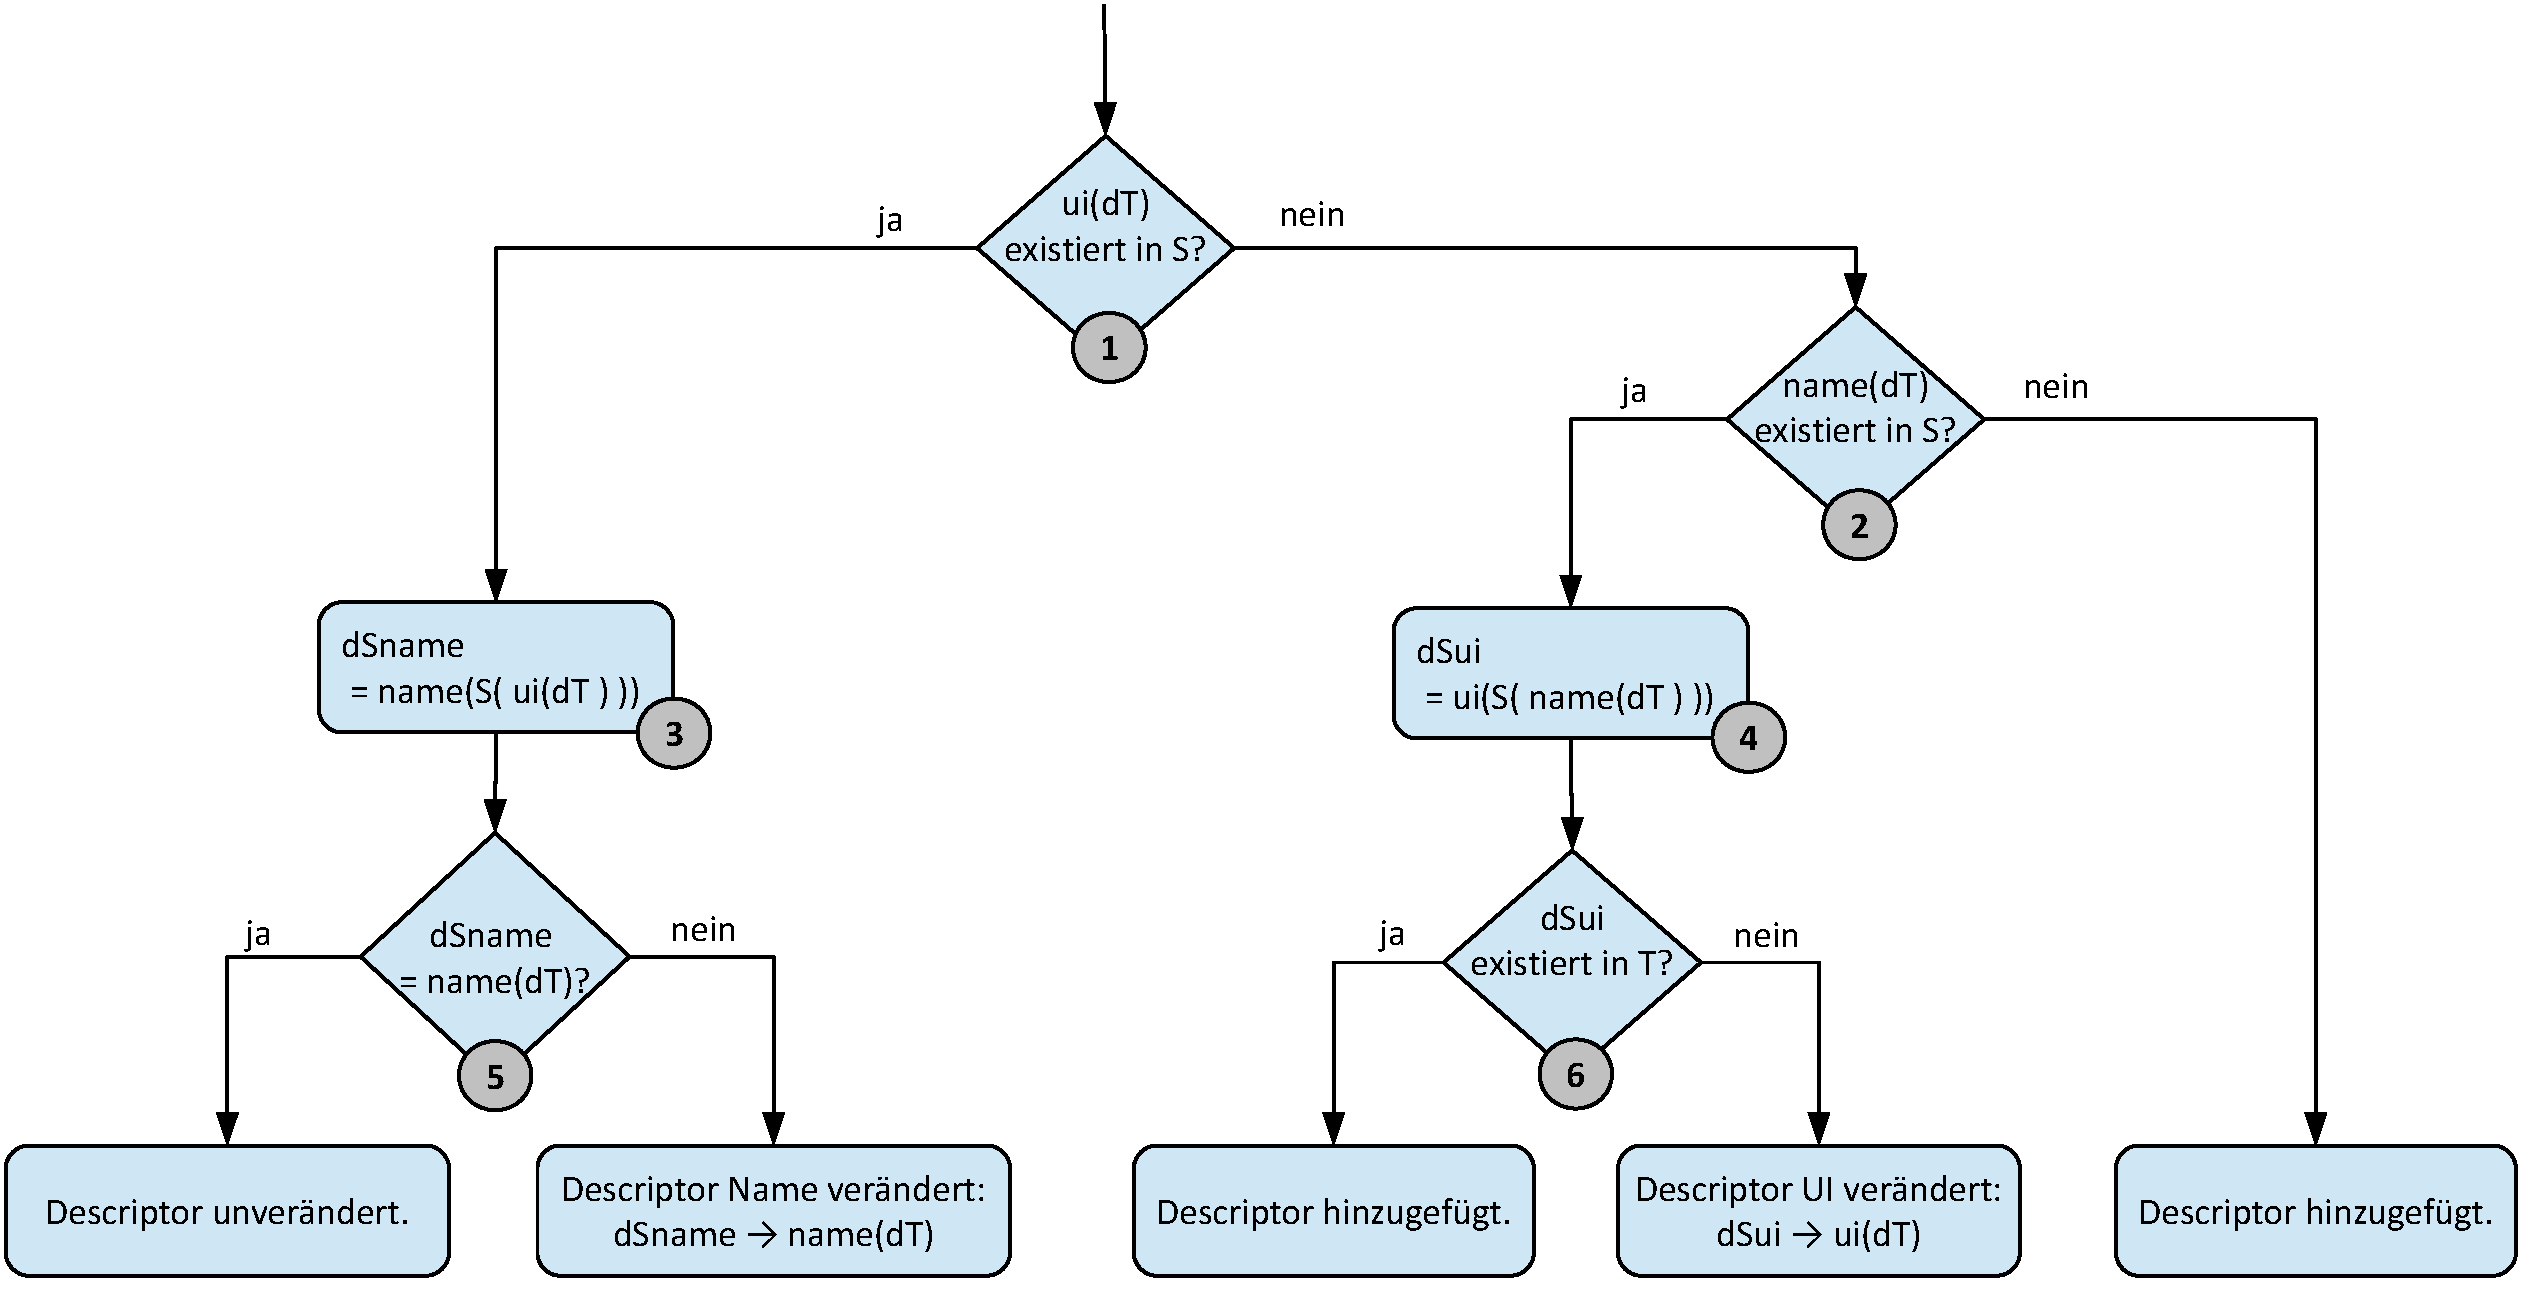
\includegraphics[width=1.05\textwidth]{figs/compare_descMods.pdf}
\end{center}
\caption{Bestimmen der Transformationen auf Descriptors}
\label{fig:compare_descMods}
\end{figure}

Es folgen Erklärungen zu den einzelnen Schritten in \autoref{fig:compare_descMods}.
\begin{enumerate}
  \item[(1)] überprüft, ob es in \code{S} einen Descriptor mit selber UI wie \code{dT} gibt.
  \item[(2)] überprüft, ob es in \code{S} einen Descriptor mit selbem Namen wie \code{dT} gibt. Wenn auch dies nicht der Fall ist, dann ist \code{dT} ein neuer Descriptor.
  \item[(3)] Für Leserlichkeit: setzt \code{dSname} gleich dem Namen des Descriptors in \code{S}, der die selbe UI wie \code{dT} hat.
  \item[(4)] Für Leserlichkeit: setzt \code{dSui} gleich der UI des Descriptors in \code{S}, der den selben Namen wie \code{dT} hat.
  \item[(5)] überprüft, ob neben der UI auch der Name \code{dT}\,s und \code{S(ui(dT))}\,s übereinstimmt. Wenn dem so ist, dann ist \code{dT} unverändert. Ansonsten hat sich der Name von \code{dSname} zu \code{name(dT)} geändert. Siehe dazu auch die Anmerkungen im nachfolgenden Abschnitt \textit{Aufteilen eines Descriptors}.
  \item[(6)] überprüft, ob es einen Descriptor \code{dS} mit UI \code{dSui} in \code{T} gibt. Ist dies der Fall, dann ist \code{dT} entstanden, indem der Name \code{dS}\,s geändert wurde. Ansonsten existiert also kein "`ähnlicher"' Descriptor in \code{S}, folglich ist \code{dS} hinzugefügt wurden. Siehe dazu auch die Anmerkungen im nachfolgenden Abschnitt \textit{Aufteilen eines Descriptors}.
\end{enumerate}

\minisec{Aufteilen eines Descriptors}
\label{sec:aufteilung_descriptor}

\begin{figure}[h]
\begin{center}
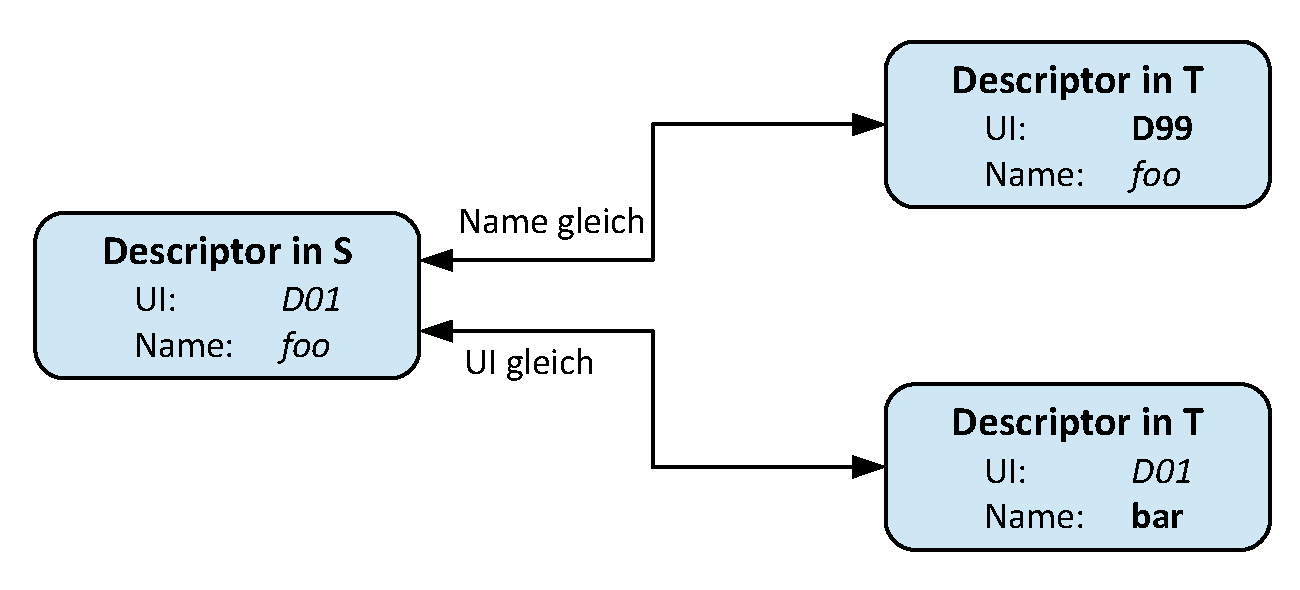
\includegraphics[width=0.7\textwidth]{figs/compare_descSplitting.pdf}
\end{center}
\caption{Descriptor-Aufteilung}
\label{fig:compare_descSplitting}
\end{figure}

Sei \code{(x,y)} für diesen Abschnitt die Bezeichnung für einen Descriptor mit UI \code{x} und Name \code{y}. Bei der Bestimmung der Descriptor-Transformationen zweier MeSH-Trees \code{S} und \code{T} kann es zu der in \autoref{fig:compare_descSplitting} gezeigten Situation kommen: Beide Descriptors aus \code{T}, \code{(D01,bar)} und \code{(D99,foo)}, sind potentiell aus \code{(D01,foo)} aus \code{S} entstanden. Wir müssen uns für der beiden Überführungsmöglichkeiten entscheiden:
%. Allerdings kann \code{(D01,foo)} nicht Operand verschiedener Transformationen sein, da es sonst zwei Transformationen geben würde, die auf \code{(D01,foo)} angewendet werden würden, was die Spezifikation aus \autoref{sec:formale_Beschreibung} verbietet. Man muss sich also für eine der beiden folgenden Überführungsmöglichkeiten entscheiden:

\begin{enumerate}
  \item Descriptor \code{(D99,foo)} ist neu. Descriptor \code{(D01,bar)} ist durch Änderung des Namens \code{(D01,foo)}\,s entstanden.
  \item Descriptor \code{(D01,bar)} ist neu. Descriptor \code{(D99,foo)} ist durch Änderung der UI \code{(D01,foo)}\,s entstanden.
\end{enumerate}

Wir entscheiden uns aus heuristischen Gründen für Variante 1: Ein Term aus \code{(D01,foo)} wurde in einen neuen Descriptor verschoben ($\rightarrow$ \code{(D99,foo)}). Dieser Term war gerade der Preferred Term, weshalb sich der Name geändert hat ($\rightarrow$ \code{(D01,bar)}). Im Gegensatz dazu sehen wir keinen Grund, warum man im MeSH die UI eines Descriptors ändern sollte.  

\subsubsection{Vertex-Neuverknüpfung}
Vertex-Neuverknüpfungen, also das Verändern, zu welchem Descriptor eine Tree Vertex gehört, sind ein Spezialfall des Vertex-Verschiebens. Dieser Sonderfall ist in \ref{sec:mesh_operationen} \textit{\nameref{sec:mesh_operationen}} dargestellt.

%Entsprechend lassen sie sich weiter in 2 Klassen einteilen: Zum einen "`Pure"' Vertex Rebindings bei denen die Tree Vertex ihren Namen behält, und zum anderen Rebindings, bei denen sich auch ihr Name ändert. Letztere werden in \ref{sec_weitere_vertex_mods} \textit{\nameref{sec_weitere_vertex_mods}} behandelt. Hier geht es ausschließlich um Pure Vertex Rebindings.\par

Wir iterieren über alle die Tree Vertices \code{vT} in \code{T}, deren Namen sich nicht geändert haben, und erkennen eine Vertex-Neuverknüpfung, falls (i) weder Name noch UI der beiden Descriptors \code{dT} und \code{dS} übereinstimmen und es außerdem (ii) kein Descriptor Relabelling bzw. Descriptor Renaming gibt, welches \code{name(dS)} in \code{name(dT)} bzw. \code{ui(dS)} in \code{ui(dT)} überführt.\par

Die erste Bedingung ist evident, da sich bei einer Vertex-Neuverknüpfung gerade der Descriptor ändert. Die zweite Bedingung erklärt sich dadurch, dass ein Umbenennen oder Relabeln eines Descriptors zwar den Descriptor verändert, nicht aber eine Vertex-Neuverknüpfung für dessen Tree Vertices darstellt. \par   

\subsubsection{Weitere Vertex-Transformationen}
\label{sec_weitere_vertex_mods}

Um alle restlichen Vertex-Transformationen zu bestimmen, traversieren wir \code{T} mittels Tiefensuche und bestimmen dann für den jeweils aktuell betrachteten Tree Vertex \code{vT} mittels des in \autoref{fig:compare_vertexMods} skizzierten Vorgehens dessen Entsprechung \code{vS} in \code{S}.\par

Es ist dabei wichtig, dass der Baum in einer solchen Reihenfolge durchlaufen wird, die garantiert, dass alle Vorfahren der aktuellen Tree Vertex bereits durchlaufen wurden. Denn an verschiedenen Stellen wird vorausgesetzt, dass der Ursprung von \code{dad(vT)} bekannt und endgültig bestimmt ist. Offensichtlich erfüllt Tiefensuche dieses Kriterium. \par  

\begin{figure}[h]
\begin{center}
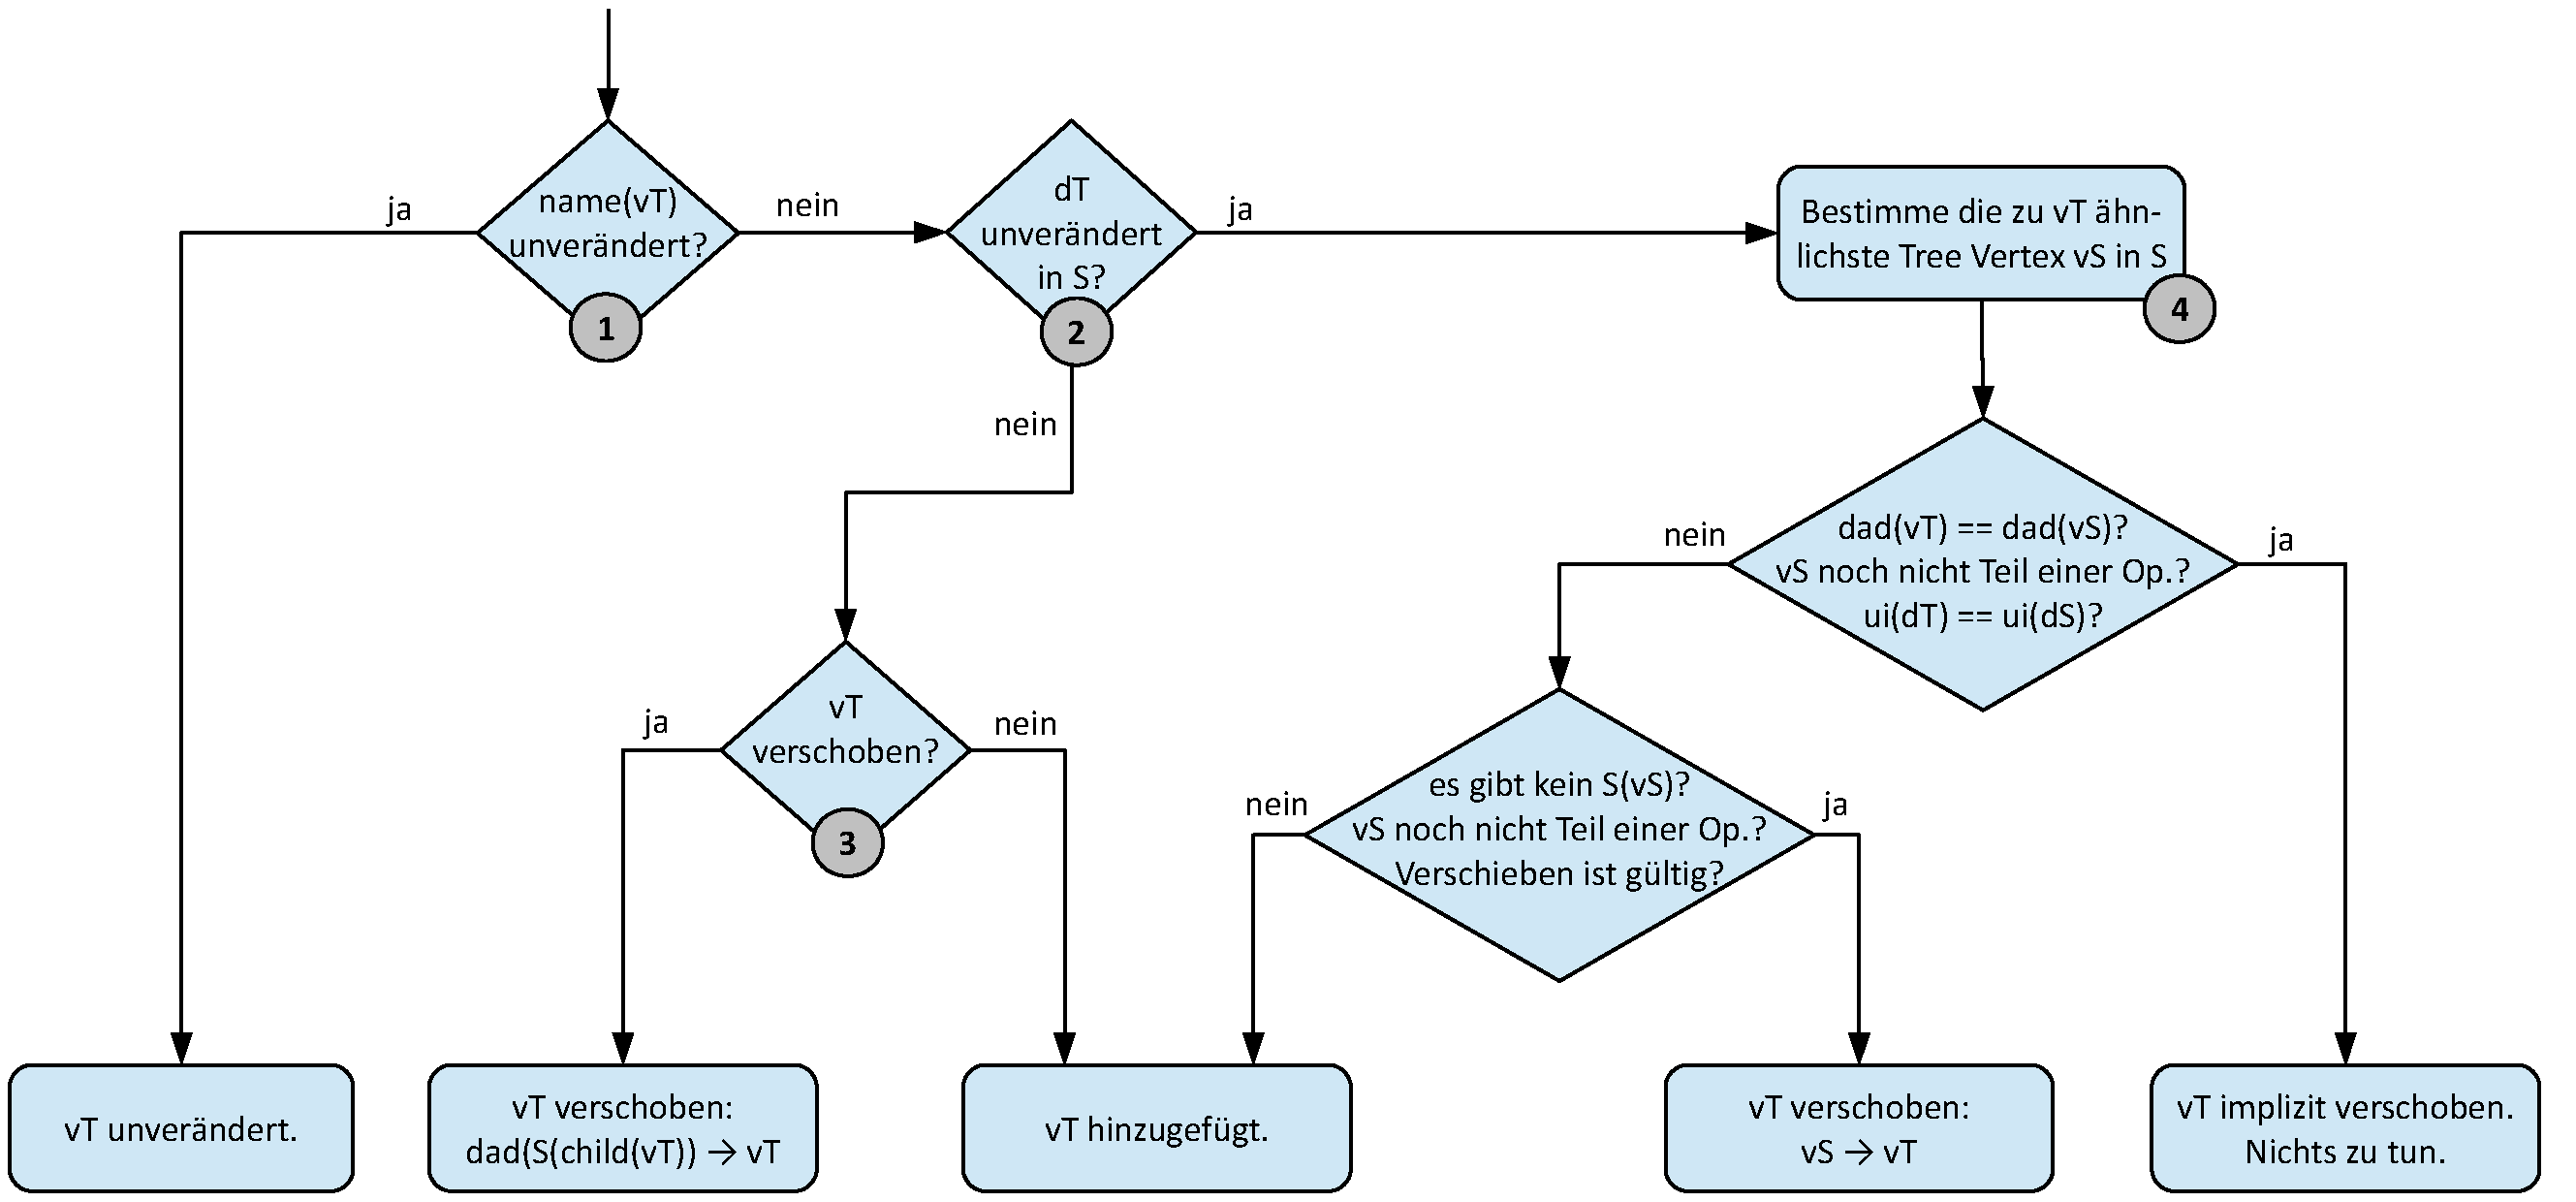
\includegraphics[width=1.05\textwidth]{figs/compare_vertexMods.pdf}
\end{center}
\caption{Bestimmen der Vertex-Transformationen}
\label{fig:compare_vertexMods}
\end{figure}

\minisec{Erläuterung von \autoref{fig:compare_vertexMods}}
% \begin{description}
% \item[\Large{\ding{172}}]% \normalsize{} Tree Vertex unverändert?]
% \end{description}

\begin{itemize}
\item[(1)] Hat sich der Name \code{vT}\,s verändert? Wenn nicht, dann hat sich auch seine Position im MeSH-Tree nicht verändert. Denn im MeSH beschreibt der Name einer Tree Vertex gerade seine Position. Wenn dies zutrifft, ist also nichts zu tun.

\item[(2)] Es wird überprüft, ob \code{dT}, also der Descriptor \code{vT}\,s, unverändert aus \code{S} übernommen wurde.

\item[(3)] %Descriptor verändert - Tree Vertex neu oder verschoben
Ist der Descriptor verändert worden, stehen wir vor einer schwierigen Aufgabe: Sowohl Descriptor als auch Tree Number \code{vT}\,s haben sich verändert. Dies sind aber die beiden wichtigsten Informationen, um herauszufinden, ob \code{vT} nun durch Verschieben oder Hinzufügen in \code{T} vorhanden ist. Es bleibt nur die strukturelle Information, d.\,h. wir analysieren die Kinder und Eltern \code{vT}\,s und versuchen daraus dessen Ursprung abzuleiten. Dabei gehen wir nach folgendem Prinzip vor:\par

\begin{itemize}
  \item[] Angenommen die Kinder \code{vT}\,s sind unverändert (d.\,h. nur implizit verschoben) und ein solches Kind sei \code{cT}.
  \item[] Wir bestimmen den Vater \code{cS}\,s, also den Vater der Entsprechung \code{cT}\,s in \code{S}, als die Tree Vertex des Descriptors \code{cS}\,s, die \code{vT} am ähnlichsten ist. Als Ähnlichkeitsmaß verwenden wir das in \ref{sec:tree_vertex_ähnlichkeit} \textit{\nameref{sec:tree_vertex_ähnlichkeit}} beschriebene. %\par
  \item[] Wenn nun \code{vT} auch in \code{S} der Vater \code{cS}\,s gewesen sein sollte, wenn \code{vT} also von dort zu seiner aktuellen Position verschoben wurde, dann müssten die \code{dad(cS)} für alle Kinder \code{cS} von \code{vT} übereinstimmen. Sollten die Eltern der Kinder in \code{S} jedoch nicht in ausreichendem Maß übereinstimmen, dann ist \code{vT} zu \code{T} hinzugefügt wurden.
\end{itemize}

%TODO Bild / weitere Erklärung \par
  
%Angenommen die Kinder \code{vT}\,s seien unverändert. Das heißt ihre Tree Number hat sich zwar verändert, aber nur weil einer ihrer Vorfahren verschobe wurde. Dann betrachten wir alle direkten Kinder \code{vT}\,s und bestimmen für jedes der \code{cT} dessen Ursprung \code{cS} (ebenfalls heuristisch).  
 

\item[(4)] %\minisec{Descriptor unverändert - Tree Vertex implizit verschoben, explizit verschoben oder hinzugefügt}  Zurück zur Fallunterscheidung zu \code{dT}.
Es existiert \code{dT} also unverändert in \code{S} als \code{dS}. Wir wollen nun den wahrscheinlichsten Ursprung \code{vT}\,s in \code{S}, also \code{vS}, bestimmen. Da \code{dT} unverändert ist, muss \code{vS} eine der Tree Vertices \code{dS}\,s sein. Wir wählen als \code{vS} jene Tree Vertex \code{dS}\,s die \code{vT} am ähnlichsten ist. Als Ähnlichkeitsmaß verwenden wir das in \ref{sec:tree_vertex_ähnlichkeit} \textit{\nameref{sec:tree_vertex_ähnlichkeit}} beschriebene. \par

Es sind nun drei Fälle zu unterschieden: 
\begin{enumerate}
  \item \code{vT} wurde implizit verschoben, das heißt sein Name (Tree Number) hat sich nur verändert, weil einer seiner Vorfahren verschoben wurde.
  \item \code{vT} wurde explizit verschoben.
  \item \code{vT} ist eine neue Tree Vertex eines existierenden Descriptor.
\end{enumerate} 

%\item[Descriptor unverändert - Tree Vertex implizit verschoben]
\textit{Fall 1} (\code{vT} wurde implizit verschoben) tritt ein, falls folgende Bedingungen erfüllt sind:
\begin{enumerate}
  \item \code{dad(vT) == dad(vS)}, d.\,h. \code{vT}\,s Vater ist gleich geblieben. 
  \item \code{ui(dT) == ui(dS)}, d.\,h. \code{vT}\,s Descriptor ist gleich geblieben. 
  \item \code{vS} ist nicht bereits Teil einer zuvor bestimmten Transformation.
\end{enumerate}

%\item[Descriptor unverändert - Tree Vertex explizit verschoben]
\textit{Fall 2} (\code{vT} wurde explizit verschoben) tritt ein, falls gilt:
\begin{enumerate}
  \item \code{vT} wurde nicht implizit verschoben.
  \item In \code{T} existiert keine Tree Vertex mit gleichem Namen wie \code{vS}, d.\,h. der zuvor bestimmte Ursprung \code{vT}\,s ist überhaupt ein möglicher Ursprung.
  \item \code{vS} ist nicht bereits Teil einer zuvor bestimmten Transformation.  
  \item \code{vS} ist kein Vorfahre der Entsprechung \code{dad(vT)}\,s in \code{S}, d.\,h. \code{vS} wird nicht nach einem Nachkommen seiner selbst verschoben. Denn das wäre keine gültige Transformation.   
\end{enumerate}

%\item[(5) Descriptor unverändert - Tree Vertex hinzugefügt]
\textit{Fall 3} (\code{vT} wurde hinzugefügt) tritt ein, falls Fall 1 und Fall 2 nicht eingetreten sind. 
%Falls \code{vT} auch nicht explizit verschoben wurde, so muss \code{vT} hinzugefügt worden sein.\par

\end{itemize}

\subsubsection{Tree-Vertex-Löschungen}
\label{sec:tree_vertex_del}
Um alle Tree-Vertex-Löschungen zu finden, gehen wir wie folgt vor: \par
Wenn ein Vertex \code{v} aus \code{S} nicht mehr unverändert in \code{T} vorkommt, und außerdem keine Transformation \code{v} in eine Tree Vertex in \code{T} überführt, dann muss \code{v} aus \code{S} gelöscht worden sein. \par
Aus diesem Vorgehen folgt unmittelbar, dass alle anderen Transformationen vor den Löschungen bestimmt werden müssen.

\subsubsection{Descriptor-Löschungen}
Das Prinzip ist analog zu dem in \autoref{sec:tree_vertex_del}: \par
Wenn ein Descriptor \code{d} aus \code{S} nicht mehr unverändert in \code{T} vorkommt, und außerdem keine Transformation \code{d} in einen Descriptor in \code{T} überführt, dann muss \code{d} aus \code{S} gelöscht worden sein.

%\subsection{Korrektheit und Optimale Lösung}
\subsection{Bewertung des Algorithmus}
Mit der hier dargestellten Vorgehensweise wird eine Transformationsfolge \code{O} gefunden, die \code{S} in \code{T} 
%entsprechend der Anforderungen aus \autoref{sec:formale_Beschreibung} 
überführt, denn:

\begin{itemize}
  \item jeder Descriptor \code{d} bzw. jede Tree Vertex \code{v} in \code{T} wird genau einmal durchlaufen.
  \item bei einem solchen Durchlaufen wird
  \begin{itemize}
    \item immer genau eine Transformation bestimmt, welche zum Auftreten von \code{d} bzw. \code{v} in \code{T} führt.
    \item keine zuvor gefundene Transformation gelöscht oder verändert.
    \item keine Transformation bestimmt, die in Widerspruch mit einer zuvor bestimmten Transformation stehen würde, d.\,h. \code{O(S)} ist zu jedem Zeitpunkt des Algorithmus' definiert.
  \end{itemize}
  \item jeder Descriptor \code{d} bzw. jede Tree Vertex \code{v} in \code{S}, die nicht durch eine zuvor ermittelte Transformation nach \code{T} übernommen wird, wird als gelöscht erkannt.
\end{itemize}

Der Algorithmus garantiert keine minimal lange Transformationsfolge, produziert aber kurze Transformationsfolgen:
\begin{itemize}
 \item Für einen Descriptor bzw. eine Tree Vertex in \code{S} welcher bzw. welche unverändert in \code{T} vorkommt, enthält \code{O} keine Transformation.
 \item Für jeden Descriptor bzw. jede Tree Vertex in \code{T} welcher bzw. welche nicht unverändert in \code{S} vorkommt, enthält \code{O} höchstens eine Transformation. 
 \item Für jeden Descriptor bzw. jede Tree Vertex in \code{S} welcher bzw. welche bei der Überführung nach \code{T} gelöscht wird, enthält \code{O} höchstens eine Transformation. 
\end{itemize}

Die Darstellungen in \autoref{sec:trans_prop} \textit{\nameref{sec:trans_prop}} motivieren die sequentielle Abarbeitung der Transformationstypen. Denn wenn eine minimal lange Transformationsfolge kommutativ ist, dann ist die Reihenfolge der Bestimmung der Transformationen der Folge beliebig.

%Die Spezifikation in \autoref{sec:formale_Beschreibung} wird also nicht erfüllt. 

%Es wird allerdings nicht unbedingt eine korrekte Lösung in dem Sinne gefunden, dass genau die Transformationen erkannt werden, die tatsächlich angewendet wurden, um $S$ nach $T$ zu überführen. Ebenso wird auch nicht unbedingt eine minimale Lösung ermittelt. Grund für beides ist, dass die verwendeten Methoden eben nur ein plausibles, "`heuristisches"' Vorgehen sind und daher nicht beweisbar korrekte bzw. minimale Ergebnisse liefern.\todo{fix!} \par
\FloatBarrier

\section{Aktualisierung von Transformationsfolgen}
\label{sec:merging}
Dieser Abschnitt behandelt das Aktualisieren von Transformationsfolgen, welches aufgrund der jährlichen Änderungen im MeSH notwendig ist, wie in \ref{sec:anual_changes} \nameref{sec:anual_changes} beschrieben.

\subsection{Problembeschreibung}
Das Aktualisierungsproblem ist in \autoref{fig:anualChangesStructure} dargestellt. Es folgt eine formalere Beschreibung:

\begin{itemize}
\item[]Seien \code{S} und \code{T} zwei MeSH-Graphen.\par

Sei \code{O} eine Folge von Transformationen, so dass \code{O(S)} = \code{S'}.\par

Gesucht ist eine Folge von Transformationen \code{O'}, so dass \code{O'(T)} = \code{T'}. Dabei soll das semantische Ergebnis der Anwendung von \code{O} auf \code{S} und \code{O'} auf \code{T} möglichst ähnlich sein.\par  
\end{itemize}

%"`ähnlich"' ist hier ein schwammiger Begriff, der sich nicht in Definitionen packen lässt.
Der Semedico-MeSH wurde nach den Erfordernissen von Semedico erstellt, wurde in diesem Sinne also nach semantischen Kriterien aus der Gesamtheit des MeSH ausgewählt. Man hat bestimmte Teile des MeSH so ausgewählt und neu angeordnet, wie es für Semedico aus inhaltlichen Gründen sinnvoll ist. Das Ziel ist es nun diese Semantik der Auswahl über die jährlichen Veränderungen des MeSHs hinaus zu erhalten -- allerdings ausschließlich auf Basis von strukturellen Veränderungen. Es findet keine inhaltliche Analyse der Descriptors oder Tree Vertices, auf die die verschiedenen Transformationen angewandt werden, statt. \par

Der Begriff der Ähnlichkeit, wie er oben in der Definition verwendet wurde, wird nachfolgend nur indirekt genauer charakterisiert, nämlich durch das in den folgenden Abschnitten beschriebene Vorgehen zur Aktualisierung der Transformationen. Dieses Vorgehen ist gerade so gewählt, dass eine aktualisierte Transformation möglichst ähnlich zur Ausgangsoperation ist.\par

Dieses Kapitel der Studienarbeit ist damit weniger als wissenschaftliche Arbeit zu sehen. Es ist allein praktisch motiviert, da ein Tool mit eben dieser Funktionalität gebraucht wird, selbst wenn es nur oberflächlich bewertet werden kann: zum einen anhand der Sinnhaftigkeit des Vorgehens und zum anderen anhand einer manuellen, qualitativen Überprüfung des Ergebnisses des Tools.

%Eine andere Formulierung des Problem wäre die folgende: Es gilt eine solche Vereinigung der Transformationsmengen \code{O} und \code{$\Delta$} zu finden, so dass \code{$\Delta$} gar nicht und \code{O} möglichst wenig verändert werden muss.

%.. Wie zuvor werden hier Heuristiken angewandt, die im allgemeinen sinnvoll erscheinen, im Einzelfall aber suboptimal sein können.

\begin{figure}[h]
\begin{center}
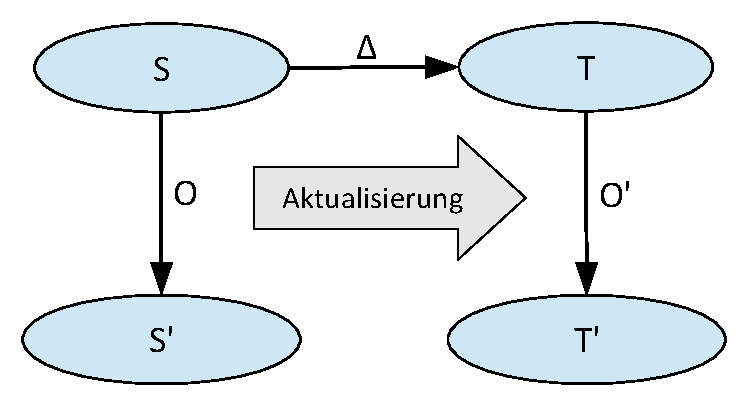
\includegraphics[width=0.6\textwidth]{figs/anualChangesStructure.pdf}
\end{center}
\caption{Aktualisierung der Transformationsfolge \code{O} für einen Ziel-MeSH-Graphen \code{T}}
\label{fig:anualChangesStructure}
\end{figure}

\subsection{Grundidee}
Das Aktualisieren der Transformationen läuft in folgenden Schritten ab:\par

\begin{enumerate}
  \item Bestimmen einer Transformationsfolge \code{$\Delta$}, welche \code{S} in \code{T} überführt
  \item Aktualisieren der Transformationen in \code{O}, als \code{O'}:
  \begin{enumerate}
    \item Descriptor-Additionen
    \item Descriptor-Umbenennungen
    \item Descriptor-Relabellings
    \item Vertex-Additionen
    \item Vertex-Verschiebungen
    \item Vertex-Löschungen
    \item Descriptor-Löschungen
    \item Vertex-Umbenennungen
  \end{enumerate}
\end{enumerate}

Zuerst bestimmen wir \code{$\Delta$}. Diese Informationen über die Änderungen, welche \code{S} in dessen neue Version \code{T} überführen, sind die Grundlage um alle Transformationen aus \code{O} zu aktualisieren. \par

Danach überführen wir alle Transformationen aus \code{O} in ihre für \code{T} angepasste Form in \code{O'}. Die prinzipielle Vorgehensweise ist dabei immer gleich: es wird über alle Transformationen eines Typs iteriert und dabei, für jede Transformation, die in den jeweilig folgenden Unterabschnitten beschriebe Heuristik angewandt. Die so aktualisierte Transformation wird dann \code{O'} hinzugefügt. \par

Die oben gegebene Reihenfolge ist bis auf eine Ausnahme beliebig: Descriptor-Additionen müssen vor Vertex-Additionen aktualisiert werden, da die Aktualisierung der Descriptor-Additionen eine Veränderung der Vertex-Additionen bewirken kann. Die restliche Reihenfolge ist beliebig, da unser konkretes Vorgehen für die verschiedenen Transformationstypen keine wechselseitigen Abhängigkeiten enthält.\par

\subsection{Vorgehen für Aktualisierung einer Transformation}
Die Aktualisierung einer Transformation \code{op} läuft immer nach dem selben Prinzip ab: \par

Man überprüft nacheinander für die einzelnen Parameter \code{op}\,s, ob diese auch in \code{T} vorhanden bzw. gültig sind. Möchte man beispielsweise eine Tree Vertex verschieben, so muss die zu verschiebende Tree Vertex in \code{T} überhaupt vorhanden sein. \par

Ist sie das nicht, wird überprüft, ob eine der Transformationen in \code{$\Delta$} dafür verantwortlich ist. Zum Beispiel könnte die Tree Vertex verschoben oder gelöscht worden sein. Wenn keine passende Transformation aus \code{$\Delta$} gefunden werden kann, wird mit einer Fehlermeldung beendet. Dieser Fall sollte nicht auftreten, da alle Veränderungen an \code{S} von \code{$\Delta$} erfasst sein sollten. Folglich ist entweder \code{$\Delta$} inkorrekt bestimmt worden, oder \code{S} oder \code{T} sind nach dem Berechnen von \code{$\Delta$} verändern worden. \par 

Wenn eine passende Transformation gefunden wurde, ist es unter Umständen möglich das Problem zu beheben. Beispielsweise verschiebt man statt der ursprünglichen, nicht mehr vorhandenen Vertex, die verschobene Vertex. Wenn kein Fix möglich ist, wird eine Fehlermeldung ausgegeben und \code{op} nicht zu \code{O'} hinzugefügt. \par

Da es erstens bei mehr als einem Parameter zu Problemen kommen kann, und zweitens auch ein Fix nicht zwangsweise zu einem gültigen Parameter führt, wiederholt man die Aktualisierung solange, bis entweder ein Fehler auftritt, der nicht gefixt werden kann, oder aber die Transformation durch die angewendeten Fixes gültig geworden ist. In letzterem Fall kann die Transformation nach \code{O'} übernommen werden.

\minisec{Bezeichnungen}
Es folgen Erläuterungen zu den Bezeichnungen in diesem Abschnitt. \par

\begin{tabular}{rl}
   \code{dad(v)} & Vater der Tree Vertex \code{v} \\
   \code{name(d)} & Name eines Descriptors \code{d} \\
   \code{ui(d)} & UI eines Descriptors \code{d} \\ \\
   \code{S(ui)} & Descriptor in \code{S} der UI \code{ui} besitzt\\
   \code{S(dname)} & Descriptor in \code{S} der Name \code{dname} besitzt\\
   \code{S(vname)} & Tree Vertex in \code{S} die Name \code{vname} besitzt\\ 
\end{tabular}  

In den Grafiken sollen die verschiedenen Farben zum Verständnis beitragen: \par
\begin{tabular}{rl}
 gelb & Einstiegspunkt. Zeigt die zu aktualisierende Transformation mit Parametern.\\
 blauer Kreis mit \code{x} & Überprüfung eines Parameters \code{x} ob dieser angepasst werden muss.\\ 
 hellblau & "`Normale"' Bedingungen und Anweisungen. \\
 grün & Erfolgreicher Abschluss der Aktualisierung. \\
 rot & Fehler.
\end{tabular}

\subsubsection{Descriptor-Additionen}

\begin{figure}[h]
\begin{center}
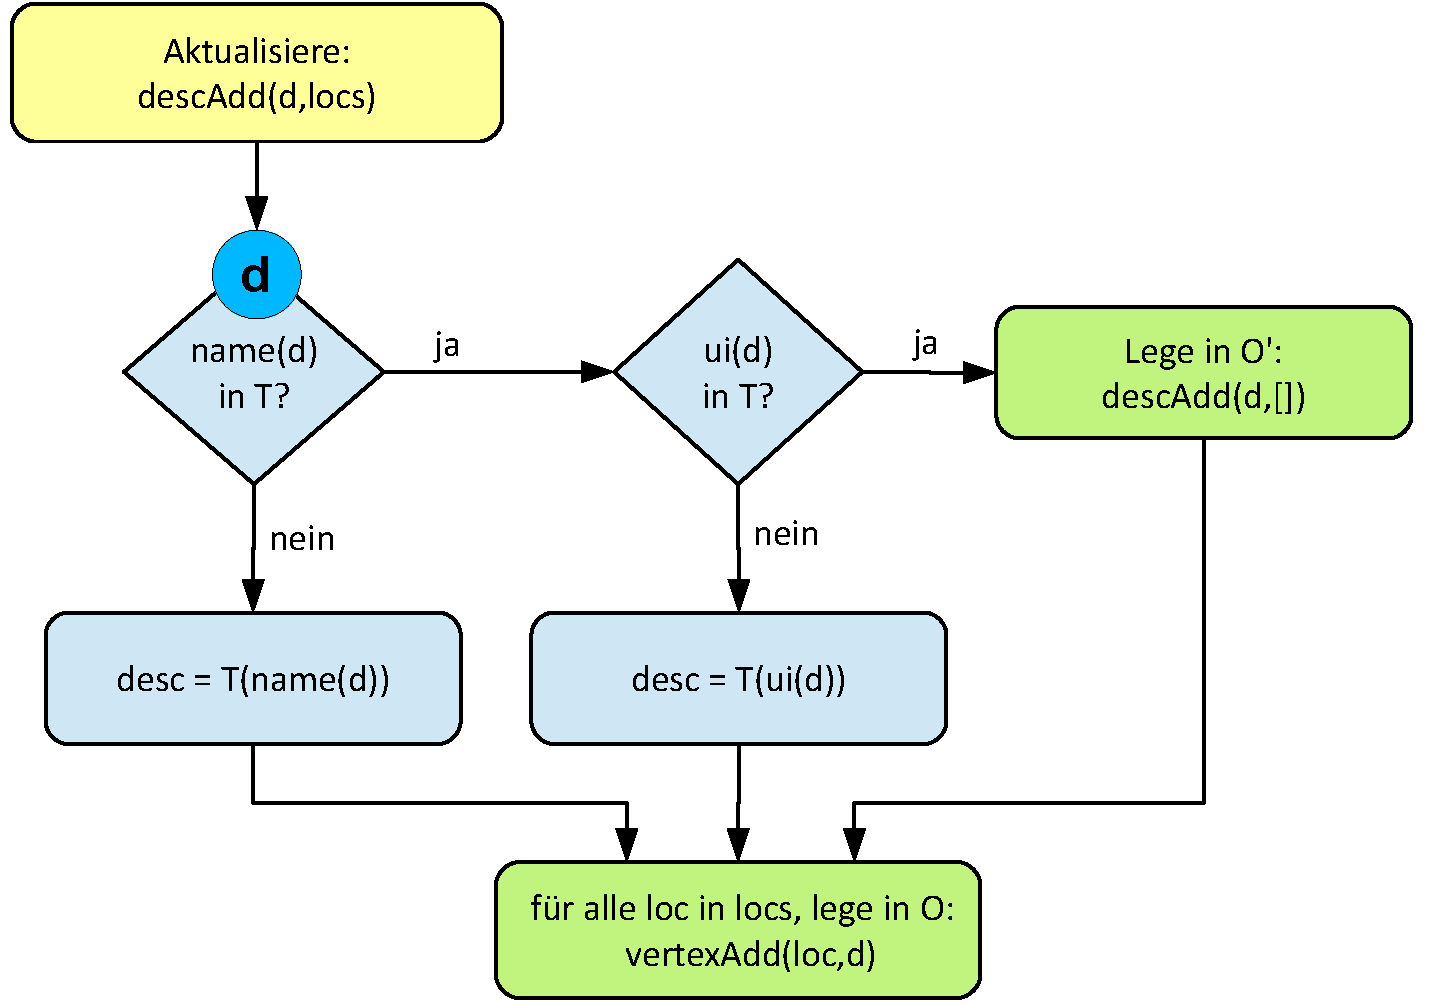
\includegraphics[width=0.8\textwidth]{figs/merge_descAdd.pdf}
\end{center}
\caption{Aktualisierung von Descriptor-Additionen}
\label{figs:merge_descAdd}
\end{figure}

Bei der Aktualisierung des Hinzufügen eines Descriptors werden immer alle Tree Vertices als separate Tree-Vertex-Additionen behandelt und diese zu \code{O} (nicht \code{O'}!) hinzugefügt. Dadurch werden die Tree-Vertex-Additionen später auf mögliche Probleme überprüft.\par

Übrig bleibt das Hinzufügen des Descriptors selbst. Wenn dessen Name oder UI bereits in \code{T} existieren, wird dieser nicht hinzugefügt. Als Descriptor für die hinzuzufügenden Tree Vertices wird dann der Descriptor des bereits existierenden Namens bzw. der bereits existierenden UI verwandt. \par

Wenn weder UI noch Name in \code{T} existieren, kann die Descriptor-Addition nach \code{O'} übernommen werden.

%Das Hinzufügen eines Descriptor muss nur aktualisiert werden, wenn entweder die UI oder der Name des hinzuzufügenden Descriptors in \code{T} bereits existieren. Ist dies der Fall, wird nicht der Descriptor selbst hinzugefügt, sondern nur die Tree Vertices. Der dazugehörige Descriptor ist dann der des bereits existierenden Namens bzw. der bereits existierenden UI. \par  

\subsubsection{Descriptor-Umbenennungen}

\begin{figure}
\begin{center}
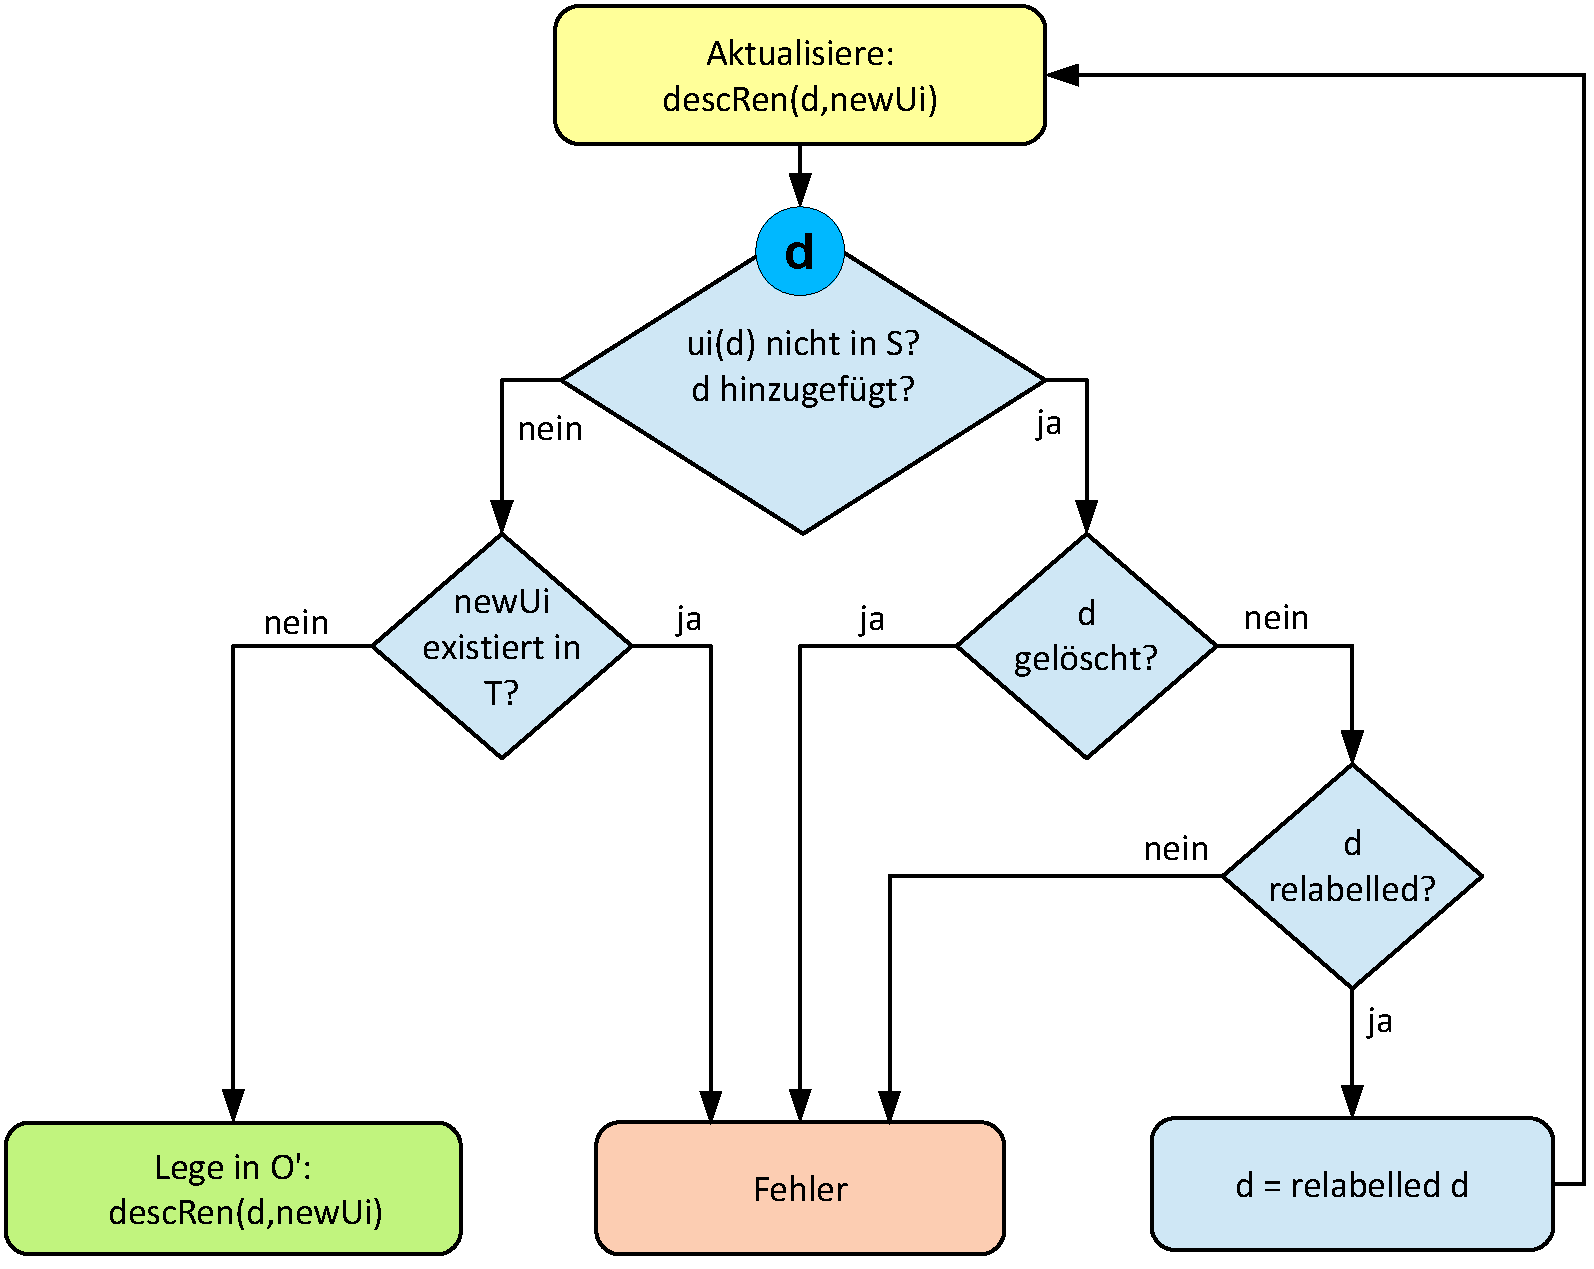
\includegraphics[width=0.9\textwidth]{figs/merge_descRen.pdf}
\end{center}
\caption{Aktualisierung von Descriptor-Umbenennungen}
\label{figs:merge_descRen}
\end{figure}
Siehe \autoref{figs:merge_descRen}.\par

Falls Descriptor \code{desc} in \code{T} bereits existiert, dann kann es zwei logische Ursachen geben:
\begin{enumerate}
  \item Der Descriptor wurde gelöscht. Dann ist eine Aktualisierung der Transformation unmöglich. 
  \item Der Descriptor hat eine andere UI bekommen. Dann verwenden wir diese veränderte UI zur abermaligen Aktualisierung der Transformation.
  \item[] Ansonsten wird ein Fehler gemeldet.
\end{enumerate}

Auch wenn \code{desc} in \code{T} nicht vorhanden ist, kann ein Problem auftreten. Nämlich, wenn die neue UI des Descriptors in \code{T} bereits vorhanden ist. In diesem Fall wird ebenfalls eine Fehlermeldung ausgegeben, da hier nicht klar ist, was getan werden sollte. 

\subsubsection{Vertex-Additionen}
Siehe \autoref{figs:merge_vertexAdd}.\par

Falls der Descriptor, zu dem eine Vertex hinzugefügt werden soll, umbenannt wurde, dann wird versucht die Vertex zu dem umbenannten Descriptor hinzuzufügen. \par

Wurde der Descriptor hingegen gelöscht, ist kein Weiterkommen und ein Fehler wird gemeldet. \par

Kann der \code{p} nicht gefunden werden, weil es gelöscht wurde, so wird stattdessen versucht \code{v} als Kind von \code{dad(p)} einzufügen. \par
 
Wenn \code{p} umbenannt wurde, fügen wir \code{v} als Kind dieser umbenannten Tree Vertex ein.

\begin{figure}
\begin{center}
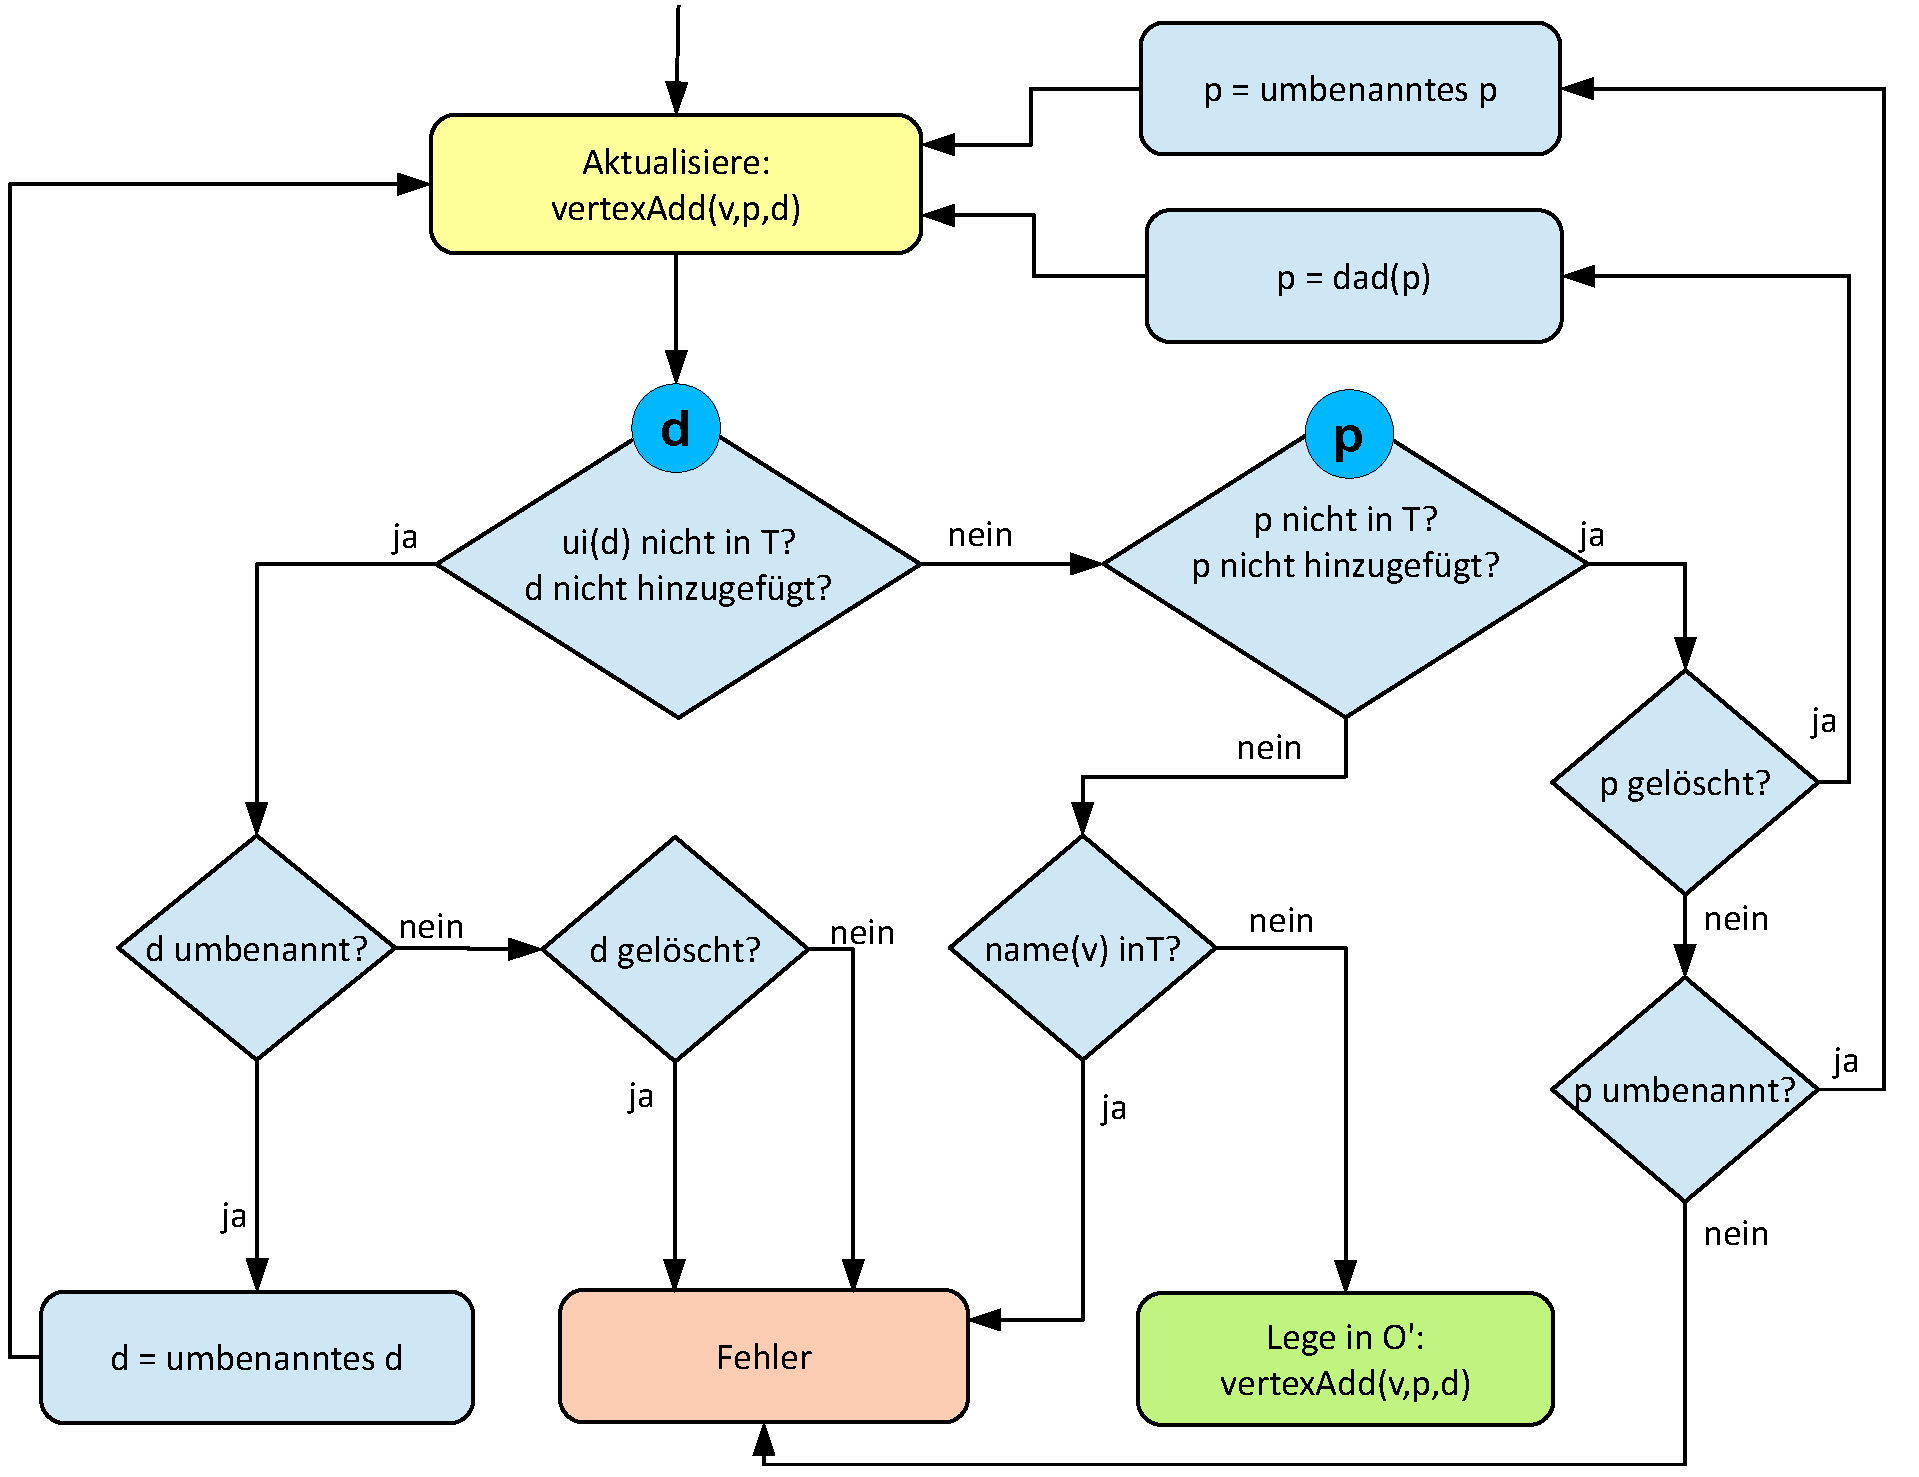
\includegraphics[width=1.1\textwidth]{figs/merge_vertexAdd.pdf}
\end{center}
\caption{Aktualisierung von Vertex-Additionen}
\label{figs:merge_vertexAdd}
\end{figure}

\subsubsection{Vertex-Verschiebungen}
Da \code{vertexMove} viele Parameter besitzt und dadurch die Grafik zu groß werden würde, ist sie in eine Übersichtsgrafik (\autoref{figs:merge_vertexMove_overview}) und 4 Teilgrafiken (\autoref{figs:merge_vertexMove_1} bis \autoref{figs:merge_vertexMove_4}) aufgeteilt worden: eine Grafik für die Problembehandlung eines jeden Parameters. \par

Die Abfragen \code{"`Aktualisierung durch x?"'} in \autoref{figs:merge_vertexMove_overview} entsprechen dem Test, ob ein Parameter \code{x} in \code{T} nicht vorhanden ist und auch nicht durch eine Transformation aus \code{$\Delta$} hinzugefügt wurde.

\begin{figure}
\begin{center}
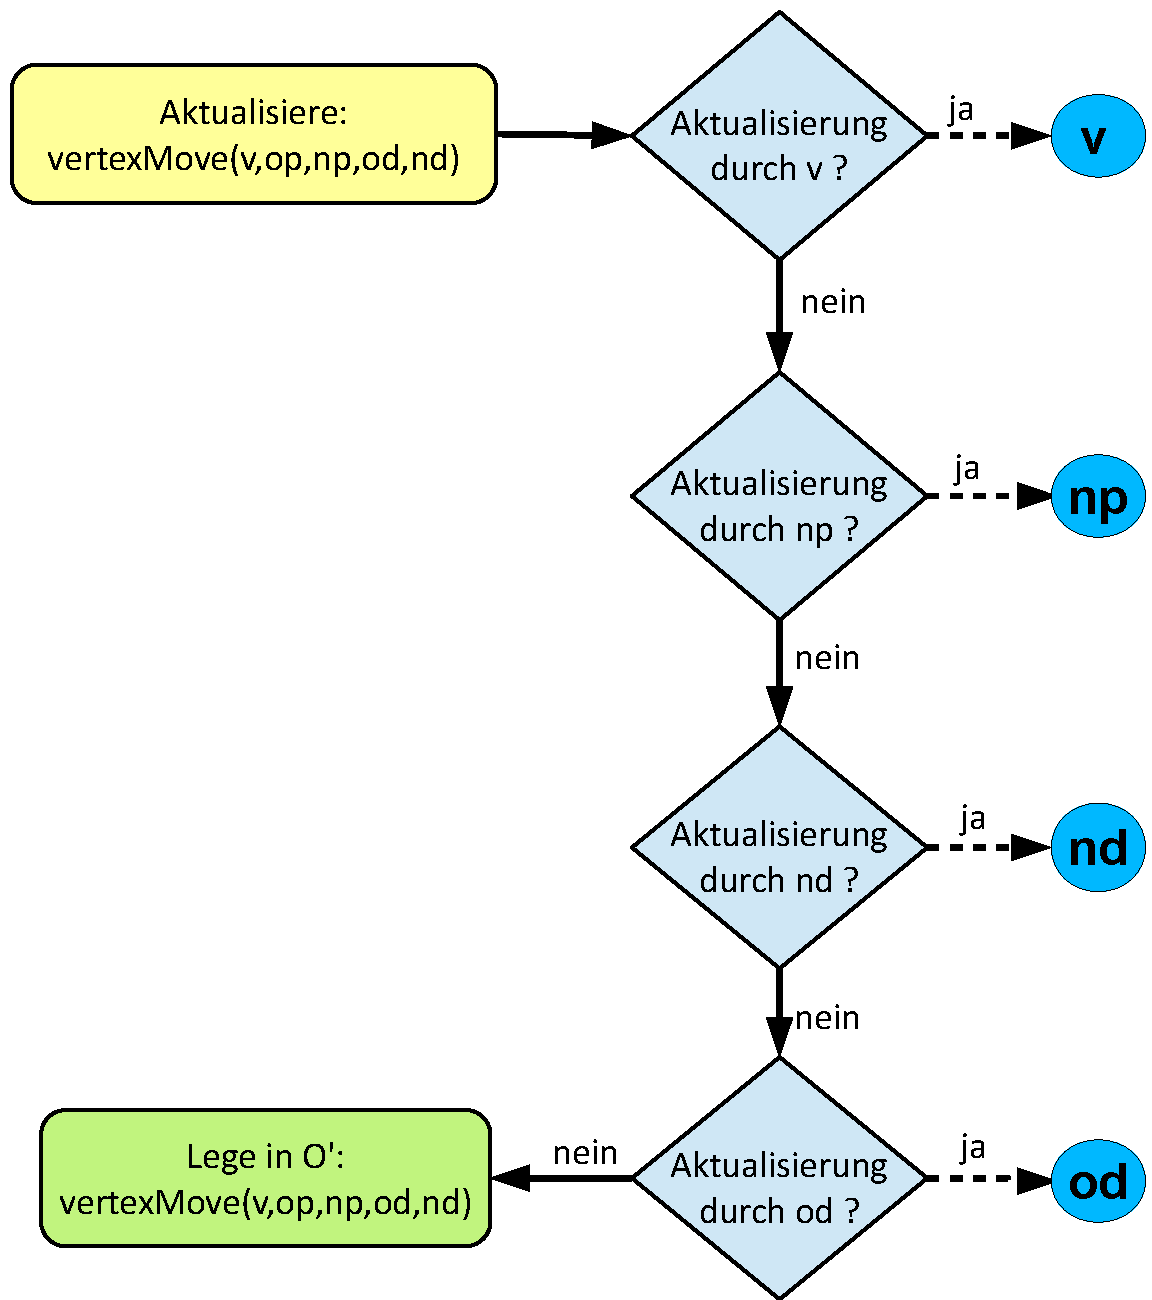
\includegraphics[width=0.6\textwidth]{figs/merge_vertexMove_overview.pdf}
\end{center}
\caption{Aktualisierung von Vertex-Verschiebungen - Übersicht}
\label{figs:merge_vertexMove_overview}
\end{figure}

Die Grafiken \autoref{figs:merge_vertexMove_1}, \autoref{figs:merge_vertexMove_2}, \autoref{figs:merge_vertexMove_3} und \autoref{figs:merge_vertexMove_4} sind weitgehend selbsterklärend. Daher folgen nur Erläuterungen zu den Schlüsselstellen. \par

\begin{figure}
\begin{center}
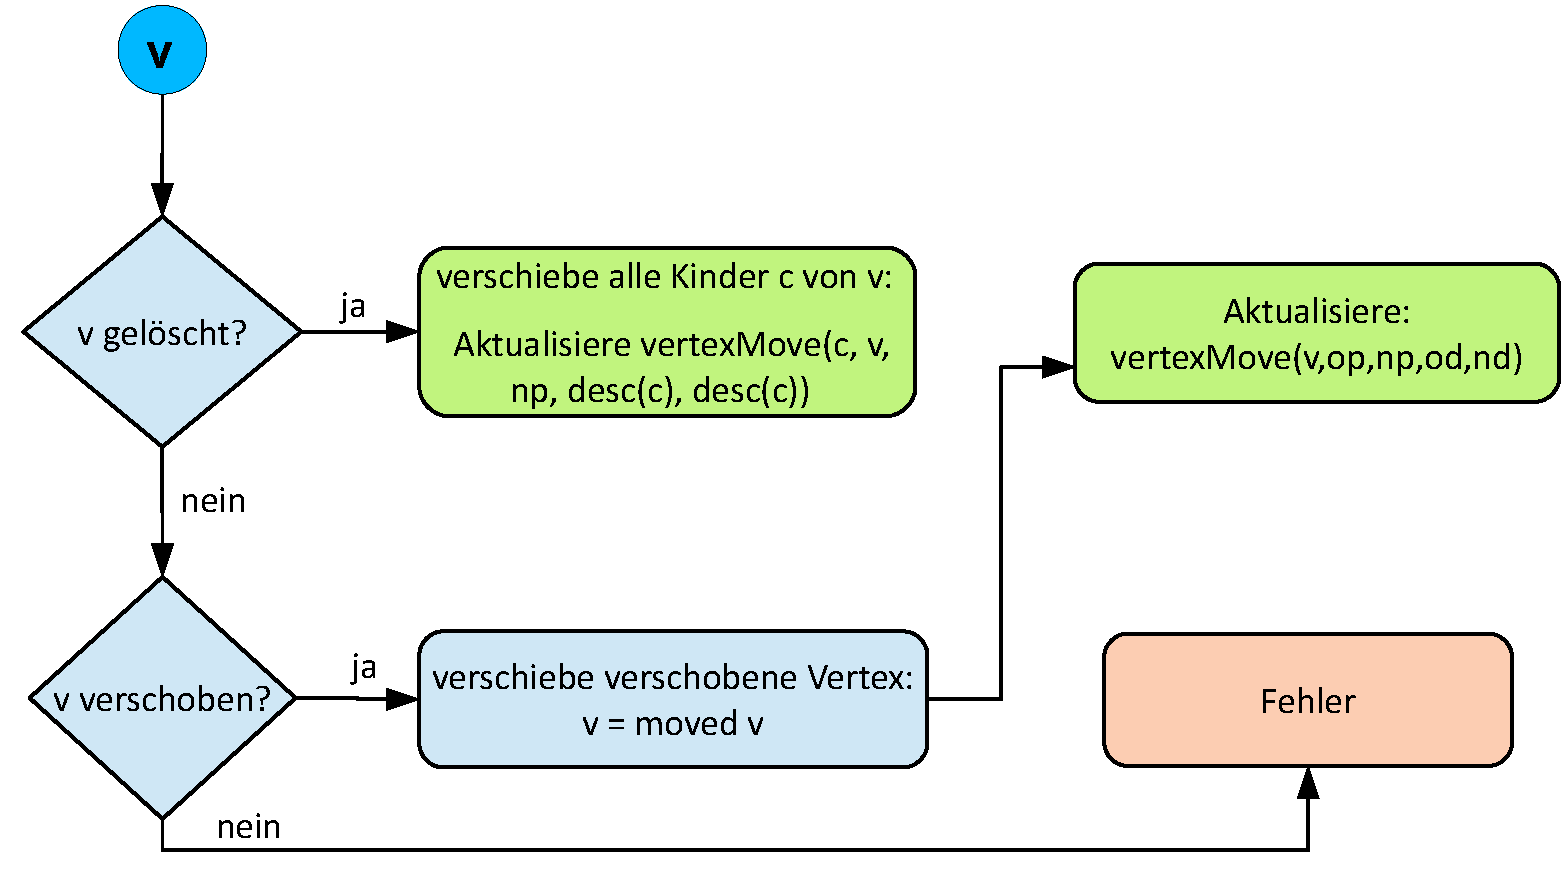
\includegraphics[width=0.7\textwidth]{figs/merge_vertexMove_1.pdf}
\end{center}
\caption{Vertex-Verschiebungen - Veränderungen an \code{v}}
\label{figs:merge_vertexMove_1}
\end{figure}

\begin{figure}
\begin{center}
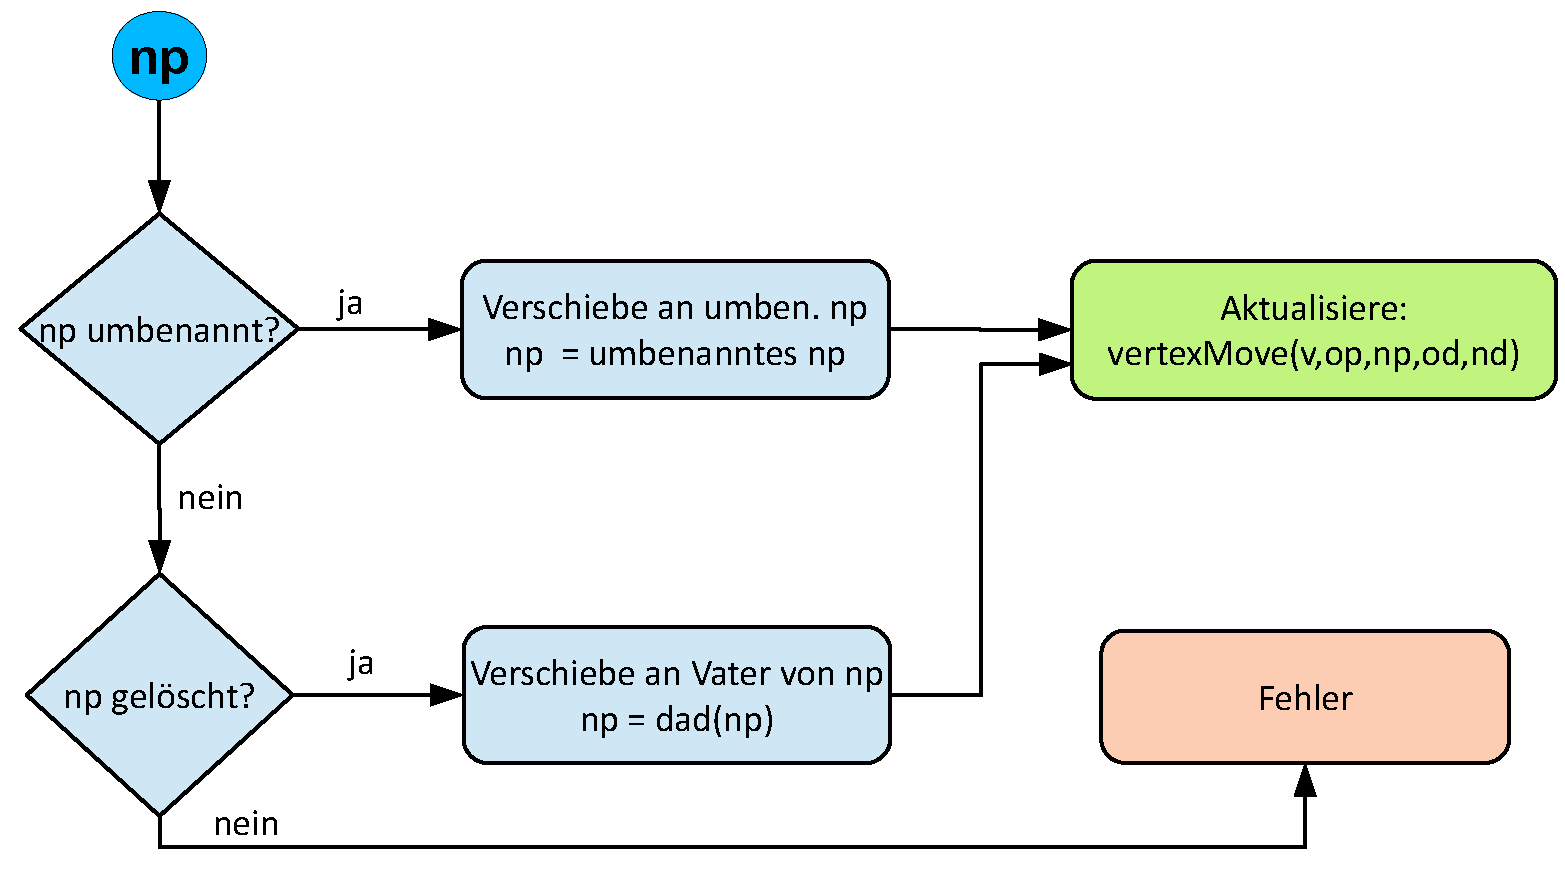
\includegraphics[width=0.7\textwidth]{figs/merge_vertexMove_2.pdf}
\end{center}
\caption{Vertex-Verschiebungen - Veränderungen an \code{np}}
\label{figs:merge_vertexMove_2}
\end{figure}

\begin{figure}
\begin{center}
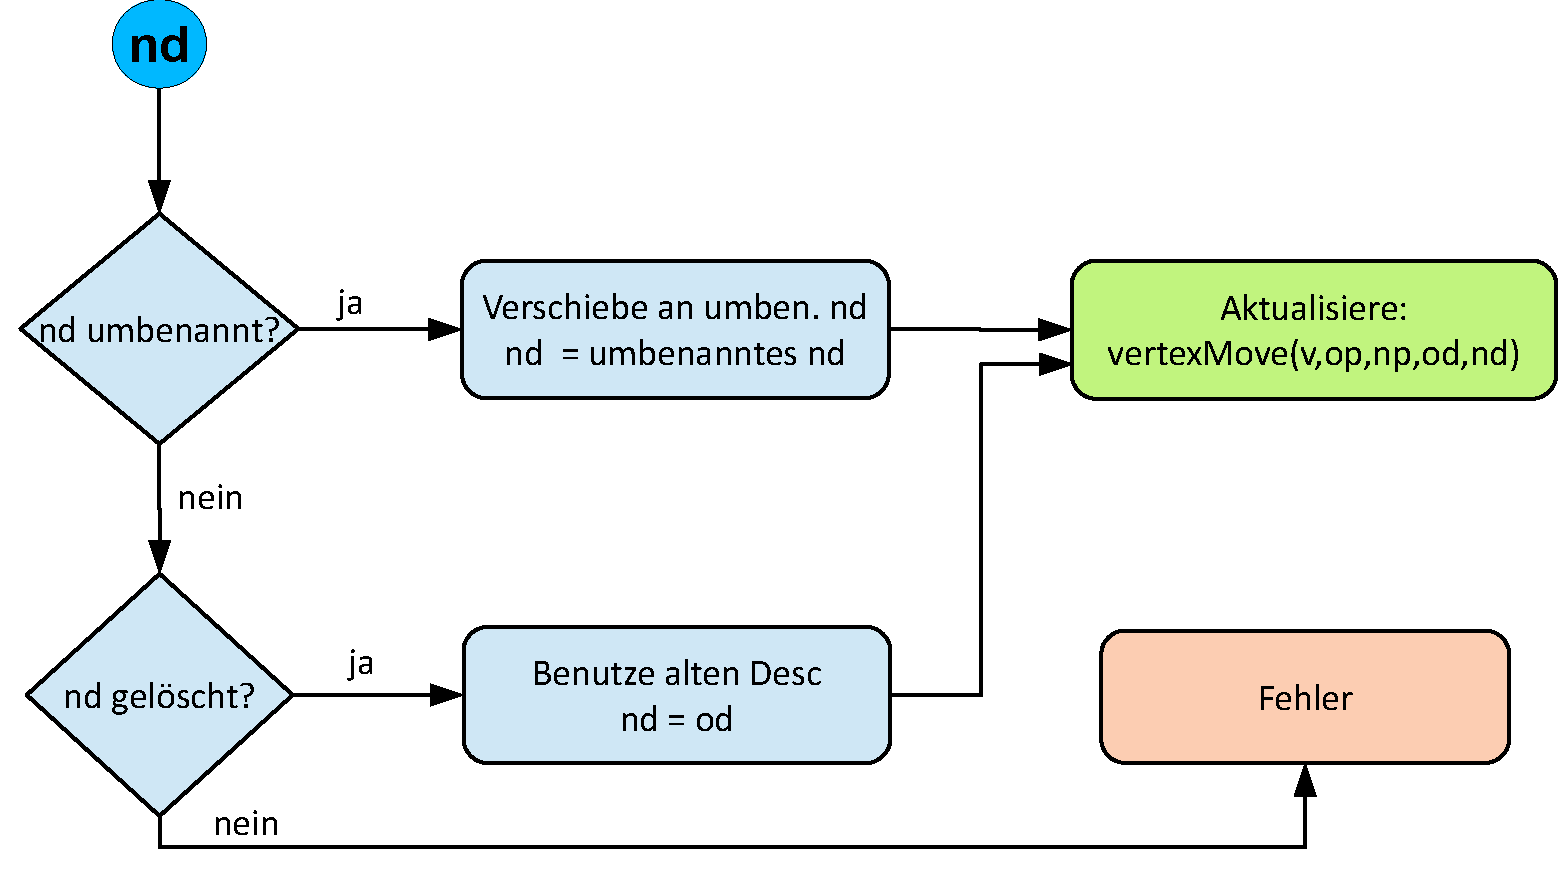
\includegraphics[width=0.7\textwidth]{figs/merge_vertexMove_3.pdf}
\end{center}
\caption{Vertex-Verschiebungen - Veränderungen an \code{nd}}
\label{figs:merge_vertexMove_3}
\end{figure}

\autoref{figs:merge_vertexMove_3}: Falls der neue Descriptor \code{nd} aus \code{T} gelöscht wurde, wird als Fix stattdessen der alte Descriptor \code{od} verwendet. Dies ist sinnvoll, da das explizite Verschieben \code{v}\,s impliziert, dass \code{v} für Semedico wichtig ist. Anstatt hier also mit einer Fehlermeldung abzubrechen, wird versucht die Transformation zu erhalten.

\begin{figure}
\begin{center}
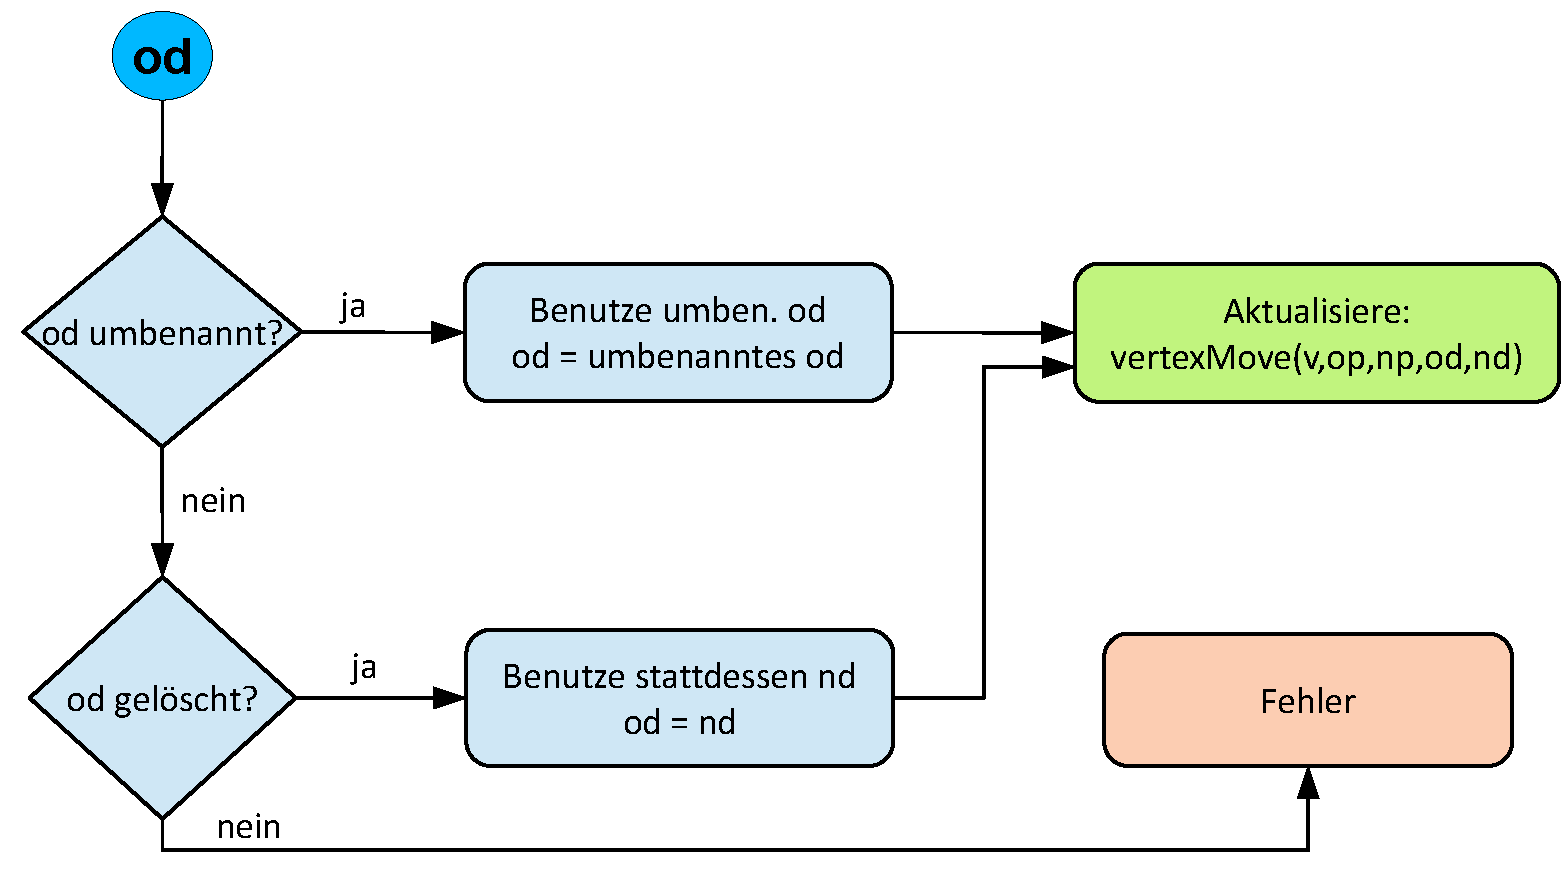
\includegraphics[width=0.7\textwidth]{figs/merge_vertexMove_4.pdf}
\end{center}
\caption{Vertex-Verschiebungen - Veränderungen an \code{od}}
\label{figs:merge_vertexMove_4}
\end{figure}

\autoref{figs:merge_vertexMove_3}: Falls der alte Descriptor \code{od} aus \code{T} gelöscht wurde, wird als Fix stattdessen der neue Descriptor \code{od} verwendet. \code{od} wird nur benötigt, um \code{od}, im Falle einer Vertex-Neuverknüpfung \code{v}\,s, zu informieren, dass \code{od} eine Tree Vertex verloren hat. Da \code{od} aber entfernt wurde, wird diese Information nicht länger benötigt und es ist korrekt \code{od} auf \code{nd} zu setzen.

\subsubsection{Vertex-Löschungen}

Siehe \autoref{figs:merge_vertexDel}. \par

Das Vorgehen ist eingängig: ist \code{v} unverändert vorhanden, kann die Vertex-Löschung direkt übernommen werden. Wurde \code{v} gelöscht, muss entweder nichts mehr getan werden, falls die Löschung nicht rekursiv war, oder es wird als Fix versucht alle Kinder \code{v}\,s zu löschen. Wurde \code{v} hingegen verschoben, so wird versucht verschobene Tree Vertex zu löschen. 

\begin{figure}
\begin{center}
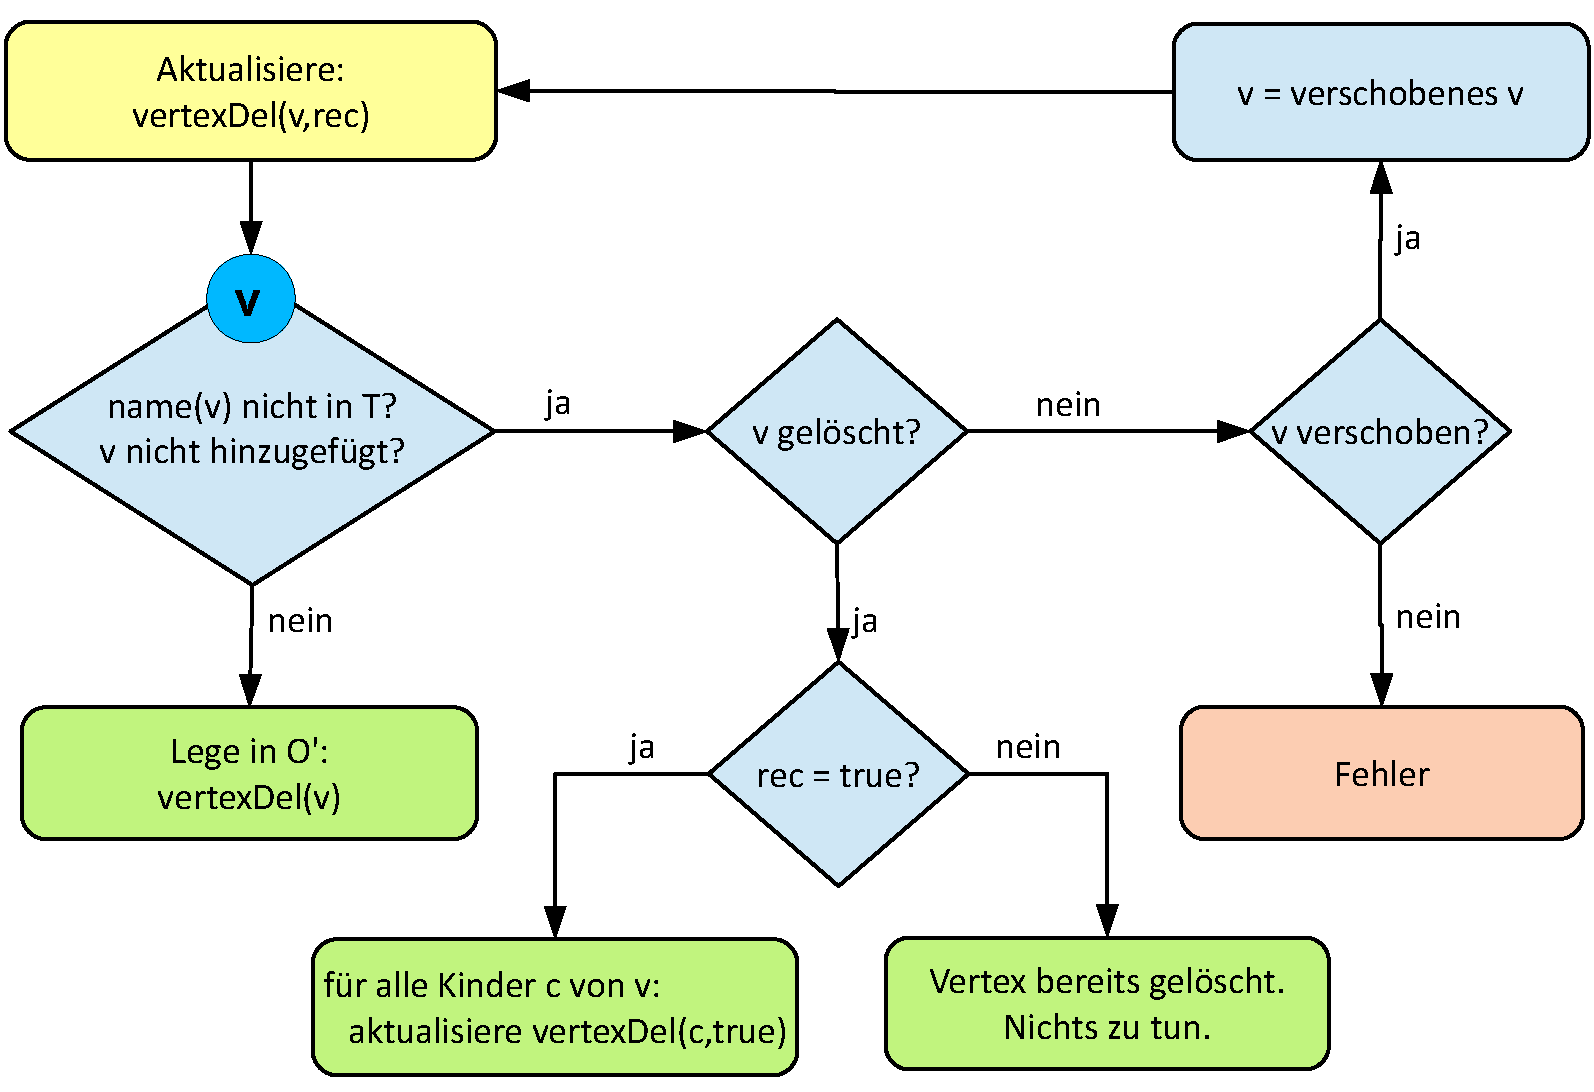
\includegraphics[width=0.80\textwidth]{figs/merge_vertexDel.pdf}
\end{center}
\caption{Aktualisierung von Vertex-Löschungen}
\label{figs:merge_vertexDel}
\end{figure}

\subsubsection{Descriptor-Löschungen}

Siehe \autoref{figs:merge_descDel}. \par 
Das Vorgehen hier ist weitgehend analog zu dem für Vertex-Löschungen.

\begin{figure}
\begin{center}
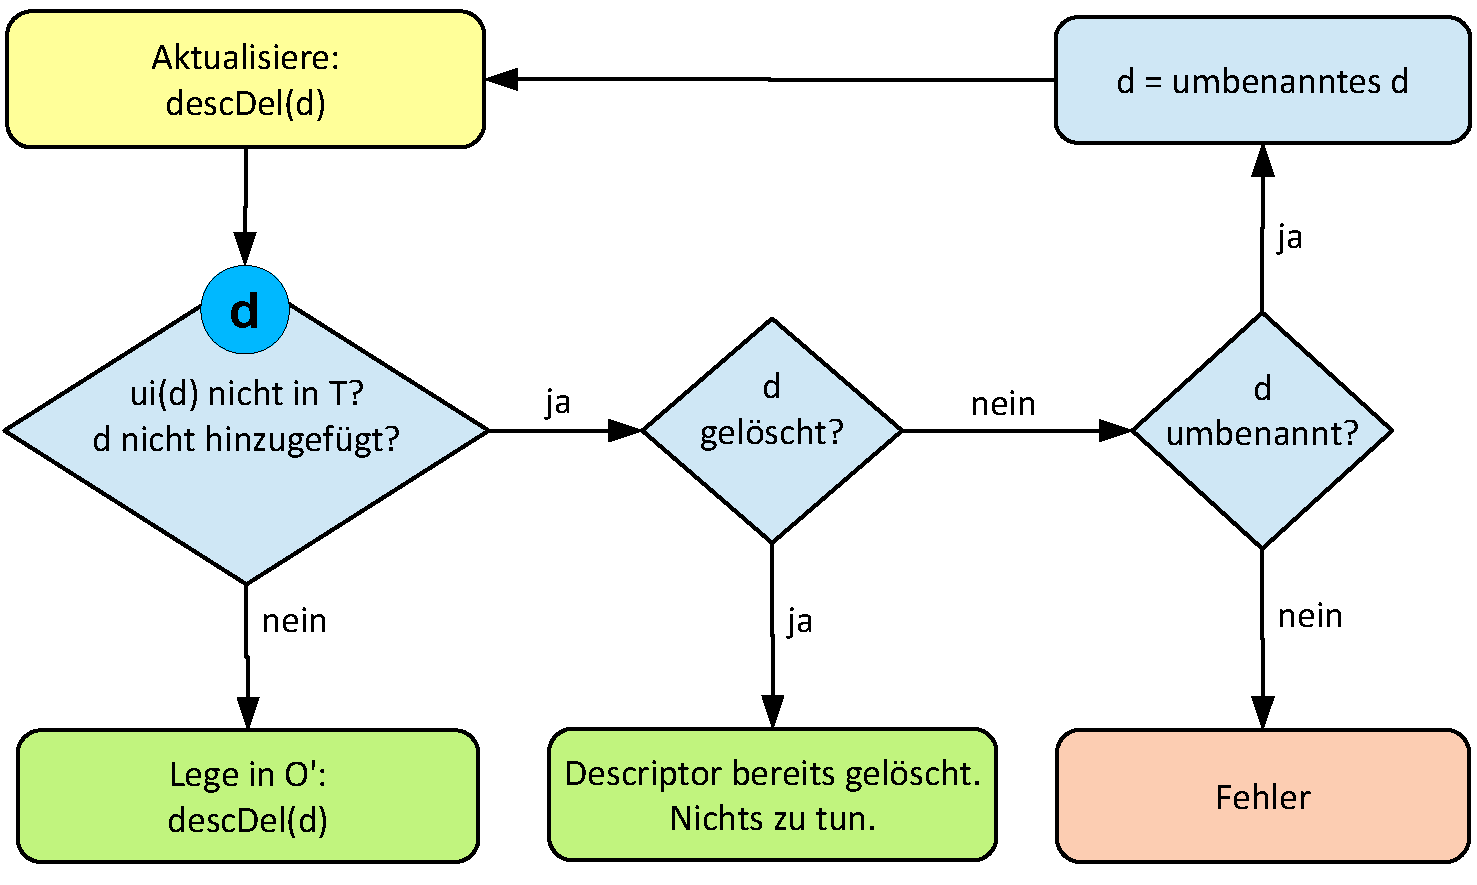
\includegraphics[width=0.8\textwidth]{figs/merge_descDel.pdf}
\end{center}
\caption{Aktualisierung von Descriptor-Löschungen}
\label{figs:merge_descDel}
\end{figure}

\subsubsection{Descriptor-Relabellings und Vertex-Umbenennungen}
Descriptor-Relabellings und Vertex-Umbenennungen treten in diesem Anwendungsfall nicht auf, da keine beim Vergleich des MeSH 2008 und des Semedico-MeSH 2008 bestimmt werden und auch nicht durch das Aktualisieren von Transformationen entstehen können. Daher wurden die beiden Transformationstypen noch nicht umgesetzt.
\FloatBarrier

\section{Umsetzung}
\label{sec:software}
Nachdem nun die Grundlagen und das prinzipielle Vorgehen zur Lösung klar sind, folgt hier eine kurze Darstellung der entwickelten Software. Zusätzlich findet sich eine ausführliche Dokumentation als Kommentare im Quelltext sowie in den Java-Doc-Pages. Bei Detailfragen sei darauf verwiesen. \par

\subsection{Wesentlichen Eigenschaften}
Folgende Richtlinien wurden bei dem Design und der Entwicklung der Software beachtet:

\begin{description}
\item[fail-early]
Die Software soll so entwickelt werden, dass die Parameter der Methoden unmittelbar auf ihren Gültigkeitsbereich überprüft werden, so dass Fehler frühzeitig erkannt und auch dem Nutzer mitgeteilt werden können. 

\item[report-early]
Die Software soll so entwickelt werden, dass sie den Nutzer möglichst gut Auskunft darüber gibt bzw. geben kann, was sie gerade tut. 

\item[Bezeichner]
Die Software soll so entwickelt werden, dass die verwendeten Bezeichner für Variablen, Methoden, Klassen und Paketen einheitlich und unmittelbar einsichtig sind, und Auskunft über die Funktion bzw. Bedeutung geben. Um lange Bezeichner zu vermeiden, werden eingängige und einheitliche Abkürzungen verwendet.\par

\item[Mehr Kommentare sind besser als weniger]
Die Software soll möglichst umfangreich und mit Hilfe von Java-Doc-Tags kommentiert werden. Das heißt, Klassen und Methoden, die sich nicht unmittelbar selbst erklären, sollen eine Beschreibung ihrer Funktion, Parameter und Besonderheiten enthalten. Zudem soll auch die interne Struktur und Funktionsweise mit Hilfe von Kommentaren begleitend erläutert werden.

\item[Frühes Abstrahieren und Kapselung]
Das Design der Software soll so geschehen, dass ein möglichst hoher Grad an Abstraktion und Kapselung erreicht wird. Das macht die Software leichter verständlich und nutzbar, erweiterbarer, wiederverwendbarer und weniger fehleranfällig.

\item[Sprache]
Die Sprache des Quellcodes und der Kommentare im Quellcode ist Englisch.
\end{description}

Dem Design lagen folgende Entscheidungen zugrunde:
\begin{description}
\item[Programmiersprache]
Da der Großteil des Semedico Projekts in Java entwickelt wurde, fiel die Wahl auch für diese Studienarbeit automatisch auf Java. \par

%Zwar interagiert die entwickelte Software im Moment nicht direkt mit Semedico, allerdings ist so gewährleistet, dass ggf. eine Integration problemlos möglich ist.

\item[Entwicklungsumgebung]
Als Entwicklungsumgebung wird Eclipse verwendet. Dies geschieht aus zwei Gründen: Erstens habe ich bereits Erfahrungen mit Eclipse und zweitens wird auch zur Entwicklung von Semedico Eclipse verwendet. 

\item[Versionsmanagement]
Da für das Semedico Projekt bereits ein SVN-Repository existiert, wurde diese, inklusive des Maven-Build-Managements, übernommen.

\item[XML-Parser]
Die XML-Daten des MeSH haben eine ungefähre Größe von 300\,MB. Daher ist es eminent wichtig einen XML-Parser zu verwenden, der erstens mit Dateien dieser Größe umgehen kann und zweitens diese auch in kurzer Zeit verarbeiten kann. \par 

Der klassische XML-Parser JDOM hat sich bei einem kurzem Test als vollkommen unbrauchbar herausgestellt. JDOM muss jederzeit ein komplettes Abbild der XML-Daten im Speicher halten und wird damit bei diesen Datenmengen extrem langsam bzw. stürzt ab. \par

Die Wahl fiel daher auf die Simple API for XML (SAX) in Form des Java-SAX-Parser, der über die Pakete \code{org.xml.sax.*} zur Verfügung gestellt wird. Dieser arbeitet sequentiell und push-event-basiert. Dadurch ist SAX deutlich schneller und minimiert den Speicherbedarf. \par

Eine mögliche Alternative ist die Streaming API for XML (StAX). Jedoch erscheint die strikt sequentielle Verarbeitungsweise von SAX hier passender und für diese Anwendung effizienter und leichter umsetzbar.

\item[Graphenbibliothek]
Als Graphenbibliothek wird die etablierte JGraphT-Bibliothek verwendet. 
\end{description}

\subsection{Design}

\begin{figure}[h]
\begin{center}
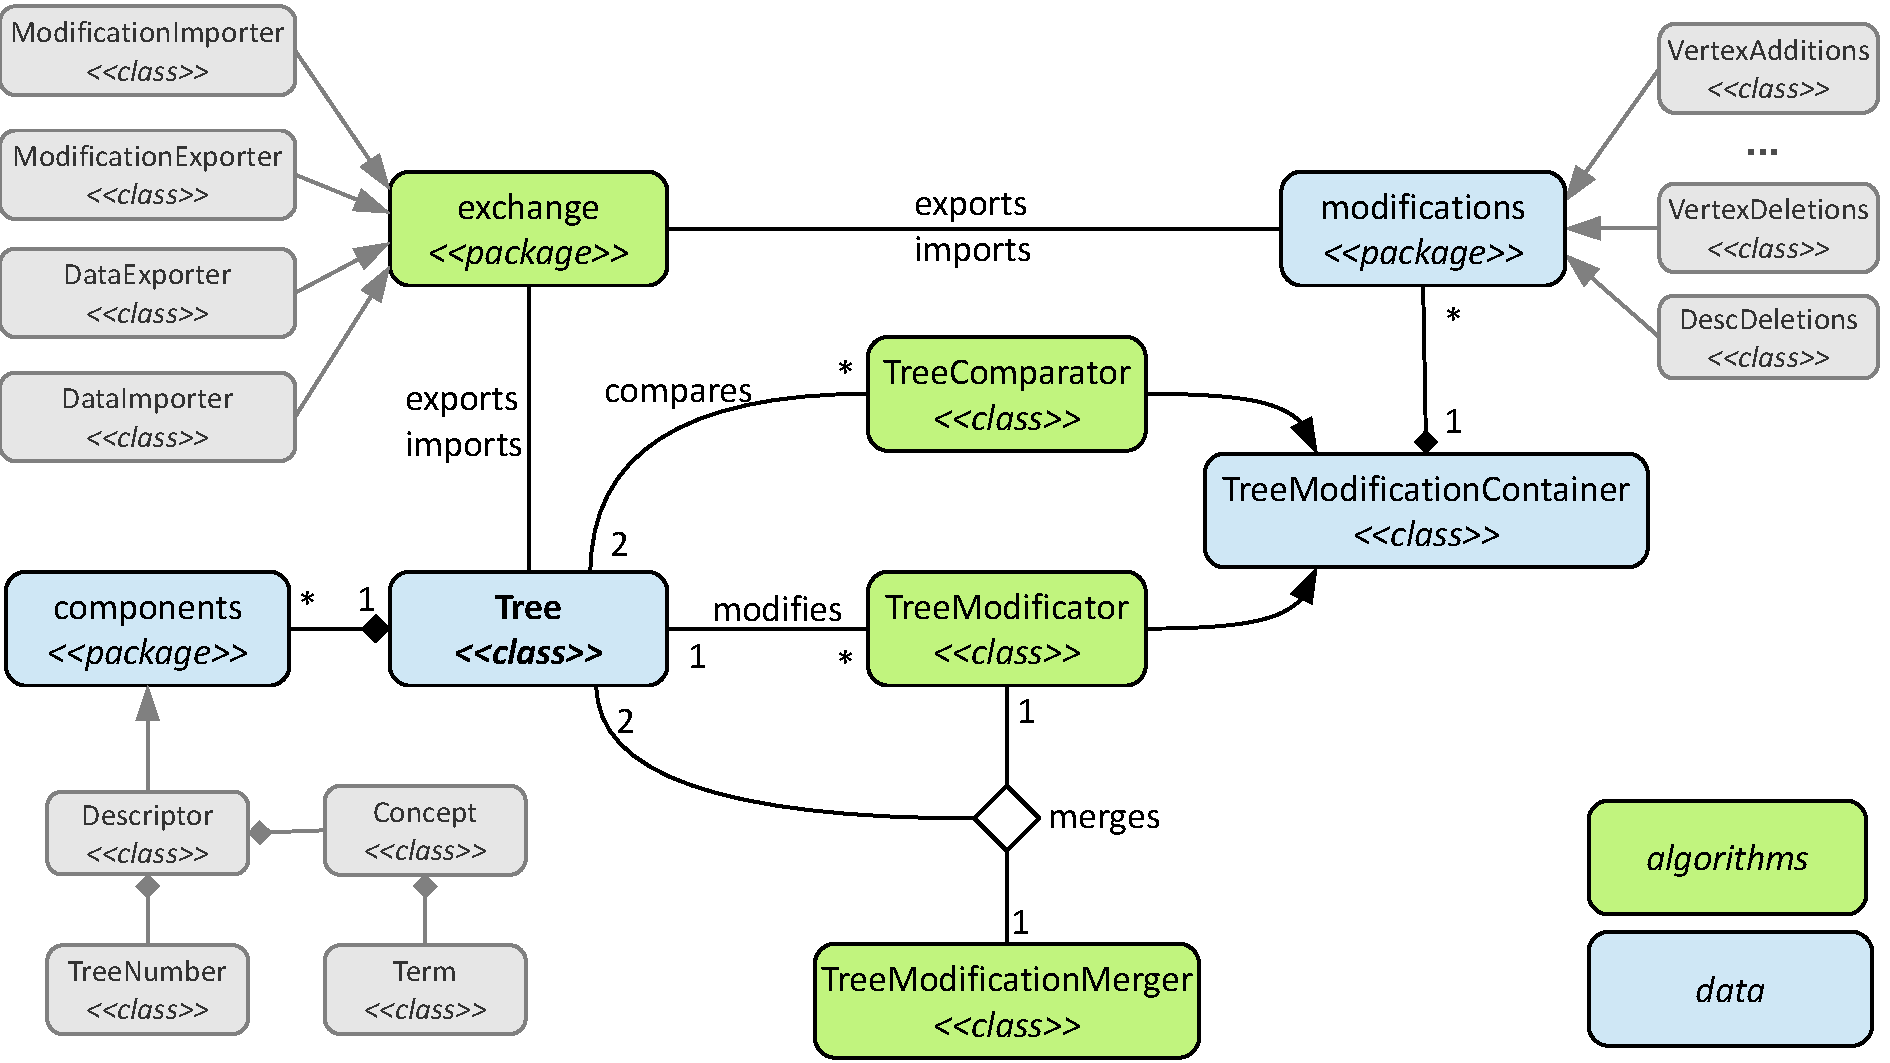
\includegraphics[width=1.0\textwidth]{figs/sw_overview3.pdf}
\end{center}
\caption{Überblick zur Struktur der Software}
\label{figs:sw_overview}
\end{figure}

\autoref{figs:sw_overview} zeigt einen Überblick zur Struktur und dem Zusammenspiel der wichtigsten Klassen und Packages. Die Darstellung ist an UML-Klassen-Diagramme angelehnt. \par

Im Zentrum steht die \code{Tree}-Klasse. Sie repräsentiert einen MeSH-Tree. \par

Der Import und Export von Modifikationen und Daten für \code{Tree} wird von Klassen im \code{exchange}-Package übernommen. \par

Unterschiede zwischen zwei MeSH-Trees können über eine Instanz der Klasse \code{TreeComparator} bestimmt werden. Diese implementieren die Algorithmen aus \ref{sec:vergleichBaume} \nameref{sec:vergleichBaume}. \par

Eine Aktualisierung von Modifikationen, wie in \ref{sec:merging} \nameref{sec:merging} beschrieben, kann durch eine Instanz der Klasse \code{TreeModificationMerger} berechnet werden.\par

Instanzen der Klasse \code{TreeModificator} erlauben es Instanzen von \code{Tree} zu verändern.\par

\code{TreeComparator} und \code{TreeModificator} leiten von der selben Basisklasse \code{TreeModificationContainer} ab, da beide ein Menge von Modifikationen verwalten. Deshalb kann das Ergebnis eines Vergleichs zweier Bäume, also ein \code{TreeComparator}-Objekt, leicht in eine Instanz von \code{TreeModificator} überführt werden, und umgekehrt. \par

Die möglichen Modifikationen entsprechen den in \ref{sec:mesh_operationen} \nameref{sec:mesh_operationen} aufgelisteten Operationen.

\subsection{Package-Übersicht}
Die Software ist in eine Reihe von Packages aufgeteilt, die jeweils für sich eine funktionale Einheit bilden. Eine Übersicht bietet \autoref{table:package_übersicht}. \par

\begin{table}[h]
\begin{center}
\begin{tabularx}{0.8\textwidth}{rX}
\toprule
\textbf{Package-Name} & \textbf{Erläuterung} \\ \midrule
Basis-Package & Enthält alle andere Pakete sowie die wesentlichen Klassen der Software. Dazu gehören insbesondere die Klassen \code{Process}, \code{Tree}, \code{TreeComparator}, \code{TreeModificator} und \code{TreeModificationMerger}. \\ \midrule
\code{components} & Beschreibt die wesentlichen MeSH-XML-Elemente, wie \code{Descriptor}, \code{Concept} oder \code{Term}, als einzelne Klassen. \\ \midrule
\code{exchange} & Für Import bzw. Export der MeSH-Daten und Modifikationen. Verschiedene Formate werden unterstützt. \\ \midrule
\code{modifications} & Beschreibt Modifikationen die auf MeSH-Trees angewandt werden können, wie \code{DescAdditions} oder \code{VertexDeletions}. \\ \midrule 
\code{testing} & JUnit-Testing-Klassen. \\ \midrule   
\code{tools} & Verschiedene Hilfsklassen und Methoden. \\ \bottomrule 
\end{tabularx}
\end{center}
\caption{Package-Übersicht}
\label{table:package_übersicht}
\end{table}

\subsection{Klassen-Übersicht}
In \autoref{table:class_übersicht} sind die wichtigsten Klassen zusammen mit ihrer Funktion aufgeführt.

\begin{table}
\begin{center}
\begin{tabularx}{1.05\textwidth}{rX}
\toprule
\textbf{Klassenname} & \textbf{Erläuterung} \\ \midrule
% \textit{Basis-Package} & \\ \midrule
%\multicolumn{2}{l}{\textit{Basis-Package}} \\ \midrule
\code{Process} & Beispielanwendung, welche die entwickelte Bibliothek nutzt. \\ \midrule

\code{Tree} & Repräsentation eines MeSH-Trees. \code{Tree} stellt elementare Methoden zum Modifizieren und Abfragen eines MeSH-Trees zur Verfügung. Dies umfasst beispielsweise Tree-Vertices löschen, verschieben oder hinzufügen. \\ \midrule
% Objekte dieser Klasse können über Methoden in \code{exchange} aus Daten unterschiedlichen Formats importiert sowie in verschiedene Formate exportiert werden. 

\code{TreeComparator} & Abstrakte Basisklasse um zwei MeSH-Trees zu vergleichen. Bestimmt dabei die Modifikationen, die den einen MeSH-Tree in den anderen überführen. \\ \midrule

\code{TreeComparatorMeSH} &  Ableitung der Klasse \code{TreeComparator}. Vergleicht zwei beliebige \code{Tree}-Instanzen. Implementiert die Methoden aus \ref{sec:vergleichBaume} \nameref{sec:vergleichBaume}. \\ \midrule

\code{TreeComparatorUD} & Ableitung der Klasse \code{TreeComparator}. Vergleich eine beliebige \code{Tree}-Instanz mit einer \code{Tree}-Instanz zu vergleichen, welche aus UD-XML-Daten (siehe \autoref{sec:sw_details}) erstellt wurde. \\ \midrule

\code{TreeFilter} & Zum Filtern von unerwünschten Tree Vertices oder Descriptors aus einem \code{Tree}-Objekt. Existiert unabhängig von den anderen Klassen zum Modifizieren.\\ \midrule

\code{TreeModificationContainer} &  Container für Tree-Modifikationen. Basisklasse für \code{TreeModificator} und \code{TreeComparator}. \\ \midrule

\code{TreeModificationMerger} & Zum Aktualisieren einer Instanz von \code{TreeModificationContainer} für ein verändertes \code{Tree}-Objekt. Implementierung der Methoden aus \ref{sec:merging} \nameref{sec:merging}.  \\ \midrule

\code{TreeModificator} &  Ableitung der Klasse \code{TreeModificationContainer}. Ermöglicht die Anwendung der enthaltenen Modifikationen auf ein \code{Tree}-Objekt. \\ \midrule

% \textit{\code{components}-Package} & \\ \midrule
% \code{Concept} & Repräsentation eines MeSH-Concepts. \\ \midrule
% \code{Descriptor} & Repräsentation eines MeSH-Descriptors. \\ \midrule
% \code{Term} &  Repräsentation eines MeSH-Terms.\\ \midrule
%\code{TreeNumber} &  Repräsentation einer MeSH-TreeNumber beim Import von MeSH-XML-Daten. Wird in \code{TreeVertex} überführt. Siehe dazu auch \ref{sec:repräsentation_des_mesh_als_baum} \nameref{sec:repräsentation_des_mesh_als_baum}. \\ \midrule
%\code{TreeVertex} & Interne Repräsentation einer MeSH-TreeNumber. \\ \midrule

%\toprule
%\textit{\code{ }-Package} & \\ \midrule
\code{DataExporter} &  Exportieren eines \code{Tree}-Objekts in verschiedene Formate. Neben dem Own-XML-Format (siehe \autoref{sec:sw_details}), wird auch ein direktes Exportieren in das Semedico-Datenbankmanagementsystem (DBMS) unterstützt. \\ \midrule
%\code{DataImporter} &  Importieren verschiedener Formate für \code{Tree}-n ein \code{Tree}-Objects in verschiedene Formate. \\ \midrule
\code{Parser4MeSH} & SAX-XML-Handler um MeSH-XML-Dokumente zu parsen. \\ \midrule
\code{Parser4OwnMeSH} & SAX-XML-Handler um Dokumente mit einer MeSH-XML-ähnlichen Syntax zu parsen. Siehe auch \autoref{sec:sw_details}. \\ \midrule
\code{Parser4UserDefMeSH} & SAX-XML-Handler um XML-Dokumente zu parsen, die mit dem alten Algorithmus zum Erstellen des Semedico-MeSH erzeugt wurden. \\ \bottomrule
\end{tabularx}
\end{center}
\caption{Klassen-Übersicht}
\label{table:class_übersicht}
\end{table}

\subsection{Interessante Details}
\label{sec:sw_details}
\minisec{XML-Formate}
Es werden im Moment drei XML-Formate unterstützt:

\begin{description}
\item[UD-XML] Der bisher zu Erstellung des Semedico-MeSH verwandte Algorithmus speichert seine Ergebnisse in einem eigenen XML-Format. Dieses Format wird hier als UD-XML bezeichnet. Die Klasse \code{Parser4UserDefMeSH} implementiert einen SAX-XML-Handler zum Einlesen. Ein Schreiben ist nicht möglich.

\item[MeSH-XML] Dies ist das offizielle und bereits in \ref{sec:xml_struktur} \nameref{sec:xml_struktur} beschrieben XML-Format des MeSH. Die Klasse \code{Parser4MeSH} implementiert den entsprechenden SAX-XML-Handler zum Einlesen. Ein Schreiben ist nicht möglich. Stattdessen kann dazu das Own-XML-Format verwendet werden. 

\item[Own-XML] Eigenes XML-Format, das eine leicht veränderte Teilmenge des MeSH-XML-Formats darstellt: \par

Nur die XML-Elemente, welche auch in \code{Tree}-Objekten repräsentiert werden, wurden übernommen. \par

Statt des XML-Elements \code{<TreeNumberList>} samt \code{<TreeNumber>}s, gibt es nun ein XML-Element \code{<LocationList>} mit den Kindern \code{<Location>}, welche selbst aus \code{<ParentVertexName>} und \code{<VertexName>} bestehen. Der Sinn ist es, die Struktur des MeSH explizit als Relation festzuhalten. Siehe dazu auch in \ref{sec:xml_struktur} den Unterpunkt Tree Number. \par
 
Die Klasse \code{Parser4OwnMesh} implementiert einen SAX-XML-Handler zum Einlesen. Schreiben ist über zwei überladene Methoden \code{toOwnXml} der Klasse \code{DataExporter} möglich.
\end{description}

\minisec{Descriptor-Additionen in \code{Tree}-Objekte}
Da die MeSH-XML-Daten als Menge von Descriptors organisiert sind, geschieht auch das Einlesen der XML-Daten als Iteration über alle \code{<DescriptorRecord>}-Elemente. Und weil Descriptors jeweils eine Menge aus Tree Vertices besitzen, und diese an beliebigen Stellen im Tree-Vertex-Baum verteilt sein können, sind wir mit einem Problem konfrontiert: Es müssen ggf. Tree-Vertices eingefügt werden, deren Väter noch nicht im MeSH-Tree existieren. \par 

Um diese Problem zu lösen, verwaltet jedes \code{Tree}-Objekt eine \code{pendingVertices}-Map: Schlüssel der Map sind die noch fehlenden Vater-Tree-Vertices. Die Werte der Map sind jeweils eine Liste der Tree Vertices, die als Kinder des Schlüssels eingefügt werden sollen. Bei jedem Einfügen einer Tree Vertex wird dann \code{pendingVertices} abgefragt, um ggf. wartende Tree Vertices tatsächlich einzufügen.

\minisec{Validierung von \code{Tree}-Objekten}
Die Klasse \code{Tree} stellt elementare Methoden zum Verändern zur Verfügung. Allerdings ist es damit möglich ein \code{Tree}-Objekt so zu modifizieren, dass die Struktur seiner Tree Vertices nicht länger einen Baum darstellt. Geschieht das auf unkontrollierte Art und Weise und wir dann versucht mit dem Objekt zu arbeiten, ist das Verhalten nicht determiniert. \par
Daher wurde die Methode \code{validataIntegrity()} implementiert, welche überprüft ob ein \code{Tree}-Objekt eine gültige Struktur hat. Dies hat sich auch während der Entwicklung als sehr hilfreich herausgestellt, da durch kontinuierliches Verwenden dieser Methode viele Fehler sehr früh entdeckt werden konnten.

\subsection{Testing}
\label{sec:testing}
Zum Testen werden in erste Linie JUnit Tests verwendet, die als Klassen im Package \code{testing} implementiert sind.\par

Folgende Tests werden für die Klasse \code{TreeComparatorMeSH} betrachtet: 
\begin{itemize}
\item ein Testfall für jeden Operationstyp, der anhand eines minimalen Beispiels überprüft, ob die zu erwartenden Modifikationen bestimmt wurden.
\item ein komplexer Testfall der alle Operationstypen involviert, bei dem analog überprüft wird, ob die entsprechenden Modifikationen bestimmt wurden.
\item ein Testfall, der die MeSH-Versionen der Jahre 2008 und 2009 vergleicht, dann die bestimmten Modifikationen auf den MeSH 2008 anwendet und im Anschluss die Gleichheit des resultierende MeSH-Trees und des MeSHs 2009 überprüft. Sind beide gleich, bestätigt dies auch für ein außerordentlich großes Beispiel die korrekte Funktionsweise des Algorithmus'. 
\end{itemize}

Zum Testen der Klasse \code{TreeComparatorUD} wird genauso vorgegangen wie beim dritten Testfall für \code{TreeComparatorMeSH}. \par

Wünschenswert wäre ein automatisches Testen der Klasse \code{TreeModificationMerger}. Ziel dieser Klasse ist es eine Menge von Modifikationen so anzupassen, dass sie auf einen veränderten MeSH-Tree angewandt werden können - \textit{und dabei die Semantik möglichst wenig zu ändern}. Weil sich eine Änderung der Semantik schwer in Zahlen fassen lässt, es vor allem schwer zu sagen ist, ob eine Aktualisierung "`richtig"' oder "`falsch"' ist, ist ein automatisches Testen mit adäquatem Aufwand nur eingeschränkt möglich. Stattdessen kann zumindest automatisiert überprüft werden ob das Ergebnis syntaktisch korrekt ist. \par 

\subsection{Benutzung}
Ziel war es eine Bibliothek zu entwickeln, die alle zu Beginn aufgeführten Ziele erfüllt und dabei möglichst flexibel sowie einfach nutzbar ist. Der normale User braucht nicht und sollte nicht wissen, welche Vorgänge im Detail im Inneren Software ablaufen. Er sollte nur wissen müssen, welche Klassen und Methoden sein konkretes Problem lösen. Ein Großteil der Bibliothek wird daher vom Endnutzer nicht direkt genutzt und soll hier auch nicht aufgeführt werden. Die genauen Schnittstellen aller Methoden sind darüber hinaus mit Java-Doc-Tags dokumentiert. \par
Als Anwendungsbeispiel wird in \autoref{lst:create2009SemedicoMesh} der vollständige Quellcode zum Erstellen des Semedico-MeSH 2009 dargestellt. Nur die Aufrufe \lstinline|getProp(...)| verweisen auf ein zuvor eingelesenes Konfigurationsfile, dass die entsprechenden Pfade einstellt.\par

\lstset{caption=Erstellen des Semedico-MeSH-2009,%
label=lst:create2009SemedicoMesh}
\begin{lstlisting}[float=htbp]
private static void create2009SemedicoMesh() {
   // parse original mesh (as of 2008)
   Tree mesh2008 = new Tree("MeSH-2008");
   DataImporter.fromOriginalMeshXml(getProp("mesh2008FilePath"), getProp("importMeshXmlDtdFilePath"), mesh2008);

   // parse semedico mesh (as of 2008)
   Tree semedico2008 = new Tree("semedico-MeSH-2008");
   DataImporter.fromUserDefinedMeshXml(getProp("semedico2008FilePath"), "no-dtd",semedico2008);

   // determine modifications
   TreeComparatorUD mods4semedico2008 = new TreeComparatorUD(mesh2008,semedico2008);
   mods4semedico2008.determineModifications();       

   // parse mesh (as of 2009)
   Tree mesh2009 = new Tree("MeSH-2009");
   DataImporter.fromOriginalMeshXml(getProp("mesh2009FilePath"), getProp("importMeshXmlDtdFilePath"), mesh2009);

   // update modifications  
   TreeModificationMerger merger = new TreeModificationMerger(mesh2008, mesh2009, mods4semedico2008);
   TreeModificator mods4semedico2009 = merger.merge();

   // apply modifications on mesh 2009 -> create semedico mesh 2009
   mods4semedico2009.applyAll(true);

   // export modifications for semedico mesh 2009       
   mods4semedico2009.saveModificationsToFiles(getProp("mods4semedico2009FilePath"));

   // export mesh 2009
   DataExporter.toOwnXml(mesh2009, getProp("semedico2009FilePath"));
}
\end{lstlisting} 




\FloatBarrier

\section{Auswertung}
%In diesem Kapitel sollen die erreichten Ergebnisse anhand der ursprünglichen Zielstellung bewertet werden. \par

Eingangs wurden in \autoref{sec:problemstellung} drei zu lösende Probleme besprochen. Diese sollen nun mit den erreichten Ergebnissen verglichen und bewertet werden. \par

\minisec{Verwaltung der Wissensbasis}
Die Software ist in der Lage den MeSH entsprechend der aktuellen Anforderungen Semedicos zu importieren, zu repräsentieren, zu modifizieren und zu exportieren. Insbesondere können die offiziellen MeSH-XML-Daten importiert und \code{Tree}-Objekte direkt in das Semedico-DMBS exportiert werden.\par

Weil Modifikationen der \code{Tree}-Instanzen als Objekte eigener Klassen dargestellt werden, ist es ebenfalls möglich, diese Modifikationen zu exportieren und zu importieren. Dadurch ist es dem Nutzer möglich kompakte, eigene Java-Programme zu schreiben, die typische Aufgaben der Wissensbasisverwaltung, wie das kontrollierte Zusammenfügen Daten verschiedener Quellen, vollautomatisiert übernehmen.\par

Weiterhin ist die \code{Tree}-Klasse reicher an Information als es die aktuelle Version Semedicos benötigt, da für Semedico im Moment nicht die vollständige Struktur des MeSH-Graphen verwandt wird, sondern nur eine vereinfachte Form. Zudem lässt sich die Software durch das Hinzufügen neuer Attribute bei Descriptors oder Tree Vertices leicht erweitern, ohne dass dazu tiefe Änderungen notwendig wären. Im Wesentlichen müssten dazu nur die Methoden zum Importieren und Exportieren angepasst werden. \par

Es ist denkbar, die Bibliothek direkt als Datenbank für Semedico zu nutzen. Statt also wie bisher die für Semedico erstellte Wissensbasis in ein separates DBMS zu exportieren, könnten alle Datenanfragen der Web-Suchmaschine direkt an \code{Tree}-Objekte gestellt werden. Dazu wären allerdings eine Reihe von Änderungen und Optimierungen bezüglich der Performance notwendig, sowie auch eine Erweiterung der Funktionalität der \code{Tree}-Klasse.\par

Da der Schwerpunkt der Studienarbeit auf dem MeSH liegt, wurden bisher keine Methoden implementiert, um Daten anderer Quellen, wie beispielsweise UniProt, zu importieren. Diese Erweiterung würde aber nur das Einlesen und Abbilden auf die \code{Tree}-Struktur umfassen und wäre mit kleinem Aufwand machbar. \par

\minisec{Vergleich von MeSH-Trees}
Die Umsetzung der Methoden aus \autoref{sec:vergleichBaume} erlauben den Vergleich \textit{beliebiger} MeSH-Trees und finden immer eine dazugehörige Transformationsfolge. Die erfolgreichen JUnit-Tests aus \autoref{sec:testing} belegen dies für den Vergleich der MeSH-Trees der Jahre 2008 und 2012: Die 2012er Daten enthalten etwa 26\,000 Descriptors und 54\,000 Tree Vertices und der Vergleich bestimmt 1\,892 Descriptor-Additionen, 81 Descriptor-Löschungen, 258 Descriptor-Umbenennungen, 11\,547 Vertex-Additionen, 2\,462 Vertex-Löschungen, sowie 798 Vertex-Verschiebungen. Wendet man diese Modifikationen auf den MeSH 2008 an, so erhält man genau den MeSH 2012 (bzw. die jeweiligen \code{Tree}-Objekte). \par

Es ist also möglich Änderungen zwischen MeSH-Versionen zu verfolgen. Auch Daten aus anderen Quellen lassen sich grundsätzlich damit vergleichen. Allerdings wäre es vermutlich sinnvoll, die Implementierung zum Vergleich von MeSH-Daten als Grundlage zu verwenden, und darauf basierend eine optimierte, d.\,h auf die Charakteristiken der Daten und dessen Veränderungen angepasste, Version des Vergleichens zu entwickeln. \par

\minisec{Aktualisierung von Transformationsfolgen}
Das Aktualisieren von Transformationsfolgen ergänzt, zusammen mit dem Vergleich von \code{Tree}-Objekten, die Verwaltungsfunktionalität. Damit ist es nicht nur möglich die Datenbasis für Semedico einmalig aus einer Reihe verschiedener Datensätze zusammenzustellen, sondern auch automatisch auf eine neue Version der jeweiligen Datensätze umzustellen. Denn das Zusammenstellen der Wissensbasis entspricht gerade der Anwendung von bestimmten Transformationen. Diese Transformationen können mit den in \autoref{sec:aktualisierung_semedico} \textit{\nameref{sec:aktualisierung_semedico}} dargestellten Methoden für eine neue Version der Daten aktualisiert werden - ohne Eingriff des Nutzers.\par

Auch hier gilt allerdings, wie im vorangegangen Abschnitt, dass es für Daten aus anderen Quellen sinnvoll scheint eine angepasste Version des Algorithmus' zu schreiben. Der Aufwand dafür sollte allerdings eher gering sein, da nur die Behandlung der verschiedenen Fälle verändert werden muss, grundsätzlich aber die Struktur und Fallunterscheidung unverändert bleibt. \par

Beim Update des Semedico-MeSHs vom MeSH 2008 auf den MeSH 2009 werden beispielsweise folgende Anzahl an Transformationen aktualisiert: 0 von 35 Descriptor-Additionen, 0 von 35 Vertex-Additionen, 131 von 246 Vertex-Verschiebungen, 1\,238 von 3\,946 Vertex-Löschungen und 22 von 19\,895 Descriptor-Löschungen.

\minisec{Zusammenfassung}
Insgesamt stellt die entwickelte Software stellt eine flexible Grundlage zur Verwaltung und Aktualisierung der Wissensbasis für Semedico dar. Die zu Beginn aufgelisteten Ziele wurden in Hinsicht auf die wichtigste Datenquelle Semedicos erreicht: Der MeSH kann importiert, verändert und exportiert werden, zudem kann der Semedico-MeSH erstellt und aktualisiert werden. 
%Arbeiten mit den Unterschiede zwischen MeSH-Trees können zuverlässig bestimmt werden.  
%Um weitere Datenquellen verwenden zu können sind nur kleine Erweiterungen der Software notwendig. 
  

\FloatBarrier
\section*{Danksagung}
\addcontentsline{toc}{section}{Danksagung} 
Ich möchte mich besonders bei meinem Betreuer Erik Fäßler bedanken, der durch unsere konstruktiven und kritischen Gespräche viel zu dem Erfolg dieser Arbeit beigetragen hat. \par

Zudem bedanke ich mich bei Prof. Dr. Clemens Beckstein für seine ausführlichen Anmerkungen zur Arbeit im Vorfeld der Abgabe. \par

Dank geht auch an Eric Bach, für sein Interesse und die langen, gemeinsamen Abende im Büro. Ohne ihn hätte es bestimmt noch länger gedauert.

\FloatBarrier
\newpage
\section*{Selbstständigkeitserklärung}
\addcontentsline{toc}{section}{Selbstständigkeitserklärung}

Hiermit versichere ich, Philipp Lucas, diese Ausarbeitung sowie die zugehörige Software selbstständig verfasst zu haben und keine anderen als die angegebenen Quellen und Hilfsmittel benutzt zu haben, sowie Zitate kenntlich gemacht zu haben. \par
\vspace{1cm}
\hfill Jena, \today \\
%\hfill Philipp Lucas \\


% Literaturverzeichnis
% wenn es nicht funktionieren sollte: sichergehen dass nicht nur pdflatex sondern auch bibtex ausgef�hrt wird! beim LED (Latex EDitor) bspw. dazu F6 dr�cken!)
% korrekte reihenfolge:
% clean -> pdflatex -> bibtex -> pdflatex -> pdflatex (ja, 2 mal!)
\newpage
\nocite{*} % auch alle nicht zitierten Quellen mit auff�hren
\printbibliography

\end{document}
